%% -*- coding:utf-8 -*-
\chapter{转换语法--最简方案}
%\chapter{Transformational Grammar -- Minimalism}
\label{Abschnitt-MP}\label{chap-mp}\label{chapter-minimalism}\label{chapter-mp}

跟上一章介绍的管辖与约束理论一样,最简方案\is{Minimalist Program (MP)|(}是由乔姆斯基在波士顿的麻省理工学院提出来的。\citet{Chomsky93b-u,Chomsky95a-u}提出,我们应该严肃地看待语言演化的问题,而且我们应该能够回答出语言知识是如何成为我们普遍认识的问题。为了回答这些问题,他认为我们应该重新关注那些语言学分析所需的最少假设的模型的理论发展上,并最终导向那些具有更少的针对个别语言内在知识的模型。
%Like\is{Minimalist Program (MP)|(} the Government \& Binding framework that was introduced in the previous chapter, the Minimalist
%framework was initiated by Noam Chomsky at the MIT in Boston. \citet{Chomsky93b-u,Chomsky95a-u}
%argued that the problem of language evolution should be taken seriously and that the question of how
%linguistic knowledge could become part of our genetic endowment should be answered. To that end he
%suggested refocusing the theoretical developments towards models that have to make minimal
%assumptions regarding the machinery that is needed for linguistic analyses and hence towards models
%that assume less language specific innate knowledge.  

与GB理论一样,最简方案也广为流传:全世界的理论家都在这一框架下工作,由此下面列出的研究者与研究机构一定是不够全面的。\emph{Linguistic Inquiry} (《语言探索》)与 \emph{Syntax} (《句法》)这两本期刊几乎只刊登最简方案的工作,而且读者可以从这些期刊中知道在该领域较为活跃的人物。
%Like GB, Minimalism is wide-spread: theoreticians all over the world are working in this
%framework, so the following list of researchers and institutions is necessarily
%incomplete. \emph{Linguistic Inquiry} and \emph{Syntax} are journals that almost exclusively publish
%Minimalist work and the reader is referred to these journals to get an idea about who is active in
%this framework. 
%% There are hotspots at the MIT (David Pesetsky and Norvin Richards), in Maryland (Norbert
%% Hornstein), and at the University of Connecticut (Željko Bošković). Mamuro Saito is a Minimalist
%% working at the Nanzan University in Japan.
%% in Europa müsste man neben Rizzi und Cinque auch Cedric Boeckx und Marcel den Dicken nennen, David Adger, Peter Svenonius, Ian Roberts, Anders Holmberg 
德语方面最为著名的学者有
Artemis Alexiadou(柏林洪堡大学)、
Günther \citet{Grewendorf2002a}(缅因的法兰克福)、
Joseph Bayer(康斯坦斯)、
和Gereon Müller(莱比锡)。
%The most prominent researchers in Germany are 
%Artemis Alexiadou, Humboldt University Berlin; 
%Günther \citet{Grewendorf2002a}, Frankfurt am Main; 
%Joseph Bayer, Konstanz; 
%and Gereon Müller, Leipzig.

尽管\xbar 理论具有极大的创新性,而且GB理论下对小句的分析具有非常重要的影响,并且可以在本书中讨论的大部分学说中找到这些内容,但是在最简方案下的技术层面的工作却非常的少。无论如何,技术层面的工作是十分有用的,因为最简方案这个框架下已经做了很多研究,而且理解该理论的基本机制可以有效地获知该理论下对语言事实的一些有趣的研究成果。
%While innovations like \xbart and the analysis of clause structure in GB are highly influential and
%can be found in most of the other theories that are discussed in this book, this is less so for the
%technical work done in the Minimalist framework. It is nevertheless useful to familiarize with the
%technicalities since Minimalism is a framework in which a lot of work is done and understanding the basic machinery makes it possible to read empirically interesting
%work in that framework.

%% The degree of formalization of Minimalist theories is not different from what is known from GB times (see
%% Sections~\ref{sec-formalization-gb}and ~\ref{sec-formalization-minimalism}) and as a result there are only few computerprocessable
%% implementations. Edward Stabler and colleagues developed so"=called \emph{Minimalist Grammars},
%% which are formalizations of some of Chomsky's and Kayne's ideas
%% \citep{Stabler2001a,Kobele2006a-u,GM2007a}. On Minimalist Grammars see also Section~\ref{sec-MG} of this
%% book. This formal work was also implemented by Stabler and others. In addition there
%% are implementations by Sandiway Fong \citep{FG2012a,Fong2014a} and \citet{NB2005a-u}. However, these implementations cover only some of
%% the aspects that are suggested in theoretical papers. They will be discussed in more detail in Section~\ref{sec-formalization-minimalism}.

尽管1980年代和1990年代的GB文献有很多相同的假设,最简方案则爆发了许多不同的方法,使得我们难以掌握。下面的内容主要参考了David Adger编著的教材之中的内容\citep{Adger2003a}。
%While the GB literature of the 1980s and 1990s shared a lot of assumptions, there was an explosion of various
%approaches in the Minimalist framework that is difficult to keep track of. The presentation that
%follows is based on David Adger's textbook \citep{Adger2003a}.

\section{表示形式的一般说明}
%\section{General remarks on the representational format}

最简方案框架下的理论假说基于GB框架下的已经完成的工作。所以,在上一章解释的很多内容可以在这一章继续讨论。但是,在基础假设方面有一些改动。该理论摒弃了最为普遍的参数原则,而是将相关区别放在特征之中。语言间的差异表现在某些特征的值上面,而且,这些特征可以是强特征,也可以是弱特征,而且特征强度也是区分不同语言的一个属性。强特征使得句法对象移向更高的位置上。读者应该对这种特征驱动的移位方法较为熟悉了,因为它是第~\ref{sec-passive-gb}节中基于移位的被动分析的一部分。在被动的GB分析中,宾语为了获得格,必须要移到IP的限定语位置上。这类由于特征值的缺失而导致的移位是最简方案中的核心部分。
%The theories that are developed in the framework of the Minimalist Program build on the work done in
%the GB framework. So a lot of things that were explained in the previous chapter can be taken over
%to this chapter. However, there have been some changes in fundamental assumptions. The general
%parametrized principles were dropped from the theory and instead the relevant distinctions live in
%features. Languages differ in the values that certain features may have and in addition to this,
%features may be strong\is{feature!strong} or weak\is{feature!weak} and feature strength\is{strength} is also a property that may vary from language
%to language. Strong features make syntactic objects move to higher positions. The
%reader is familiar with this feature"=driven movement already since it was a component of the movement"=based
%analysis of the passive in Section~\ref{sec-passive-gb}. In the GB analysis of passive, the object
%had to move to the specifier position of IP in order to receive case. Such movements that are due to
%missing feature values are a key component in Minimalist proposals.

\subsection{基本框架}
%\subsection{Basic architecture}

乔姆斯基提出,只有两条操作(规则)用来整合语言对象:外部合并与内部合并。外部合并是指将\emph{the}和\emph{book}这两类元素组合起来,从而得到一个复杂的短语。内部合并被用来指称组成成分的移位。它应用于一个语言对象,并且从这个语言对象中取出一部分,并将之链接到对应对象的左边。外部合并与内部合并的应用可以按照任意顺序来实现。比如说,两个对象可以按照外部合并组合起来,然后一个合并项通过应用内部合并而移动到左边。得到的对象可以再与其他对象进行外部的合并,并且继续合并。如例(\mex{1})所示:
%Chomsky assumes that there are just two operations (rules) for combining linguistic objects:
%External and Internal Merge. External Merge simply combines two elements like \emph{the} and
%\emph{book} and results in a complex phrase. Internal Merge is used to account for movement of
%constituents. It applies to one linguistic object and takes some part of this linguistic object and
%adjoins it to the left of the respective object. The application of External Merge and Internal
%Merge can apply in any order. For instance, two objects can be combined with External Merge and then
%one of the combined items is moved to the left by applying Internal Merge. The resulting object can
%be externally merged with another object and so on. As an example consider the NP in (\mex{1}):
\ea
\gll the man who we know\\
DET 男人 CONJ 我们 认识\\
\glt `我们认识的那个男人'
\z
为了得到这个NP,动词know(认识)与它的宾语who(谁)通过外部合并在一起。在下面讨论的几个中间过程的合并之后,know who将与we合并,最后who通过内部合并移到左边,得到了who we know。这个关系小句还可以通过外部合并与man组合在一起,并且继续进行下去。
%To derive this NP the verb \emph{know} is externally merged with its object \emph{who}. After
%several intermediate merges that will be discussed below, \emph{know who} will be merged with
%\emph{we} and finally the \emph{who} is moved to the left by Internal Merge, resulting in \emph{who
%  we know}. This relative clause can be externally merged with \emph{man} and so on.

\addlines
所以,最简方案与GB理论是不同的,它没有假定一个通过某个\xbar 语法生成的深层结构以及通过\movea 从深层结构生成的表层结构。相反,它假定短语是由外部合并和内部合并(组合与移位)按照任意顺序生成一个结构,然后就被拼写出来。结构被发送到表层:一方面是发声-感知系统(AP),另在一方面是感知-意念系统(CI)。AP对应于GB理论中的音位形式(PF)层,CI对英语逻辑形式(LF)层。图~\vref{fig-architecture-minimalism}描述了这种新的架构。
%So, Minimalist theories differ from GB in not assuming a Deep Structure that is generated by some
%\xbar grammar and a Surface Structure that is derived from the Deep Structure by \movea. Instead, it
%is assumed that there is a phase in which External and Internal Merge (combination and movement)
%apply in any order to derive a certain structure that is then said to be spelled out. It is said
%that the structure is sent to the interfaces: the articulatory-perceptual system (AP) on the one hand and
%the conceptual-intentional system (CI) on the other side. AP corresponds to the level of
%Phonological Form (PF) and CI to the level of Logical Form (LF) in GB. The new architecture is
%depicted in Figure~\vref{fig-architecture-minimalism}.
\begin{figure}
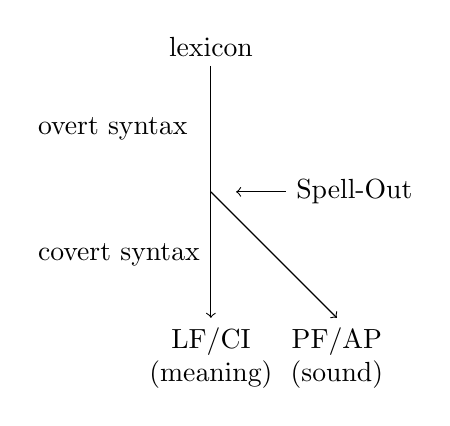
\begin{tikzpicture}[scale=.8]
%\draw (-2.9,-5.8) to[grid with coordinates] (2.7,-0.6);
\draw[->] (0,-1) node[anchor=south] {lexicon} --(0,-5) node[anchor=north, align=center] {LF/CI\\(meaning)};
\draw[->] (0,-3)--(2,-5) node[anchor=north,align=center] {PF/AP\\(sound)};
\draw[<-] (.4,-3)--(1.2,-3) node[anchor=west] {Spell-Out};
%\draw (0,-0.5) node {lexicon};
\draw (-2.9,-2) node[anchor=west] {overt syntax};
\draw (-2.9,-4) node[anchor=west] {covert syntax};
%\draw (0,-6.5) node[align=center] {LF/CI\\(meaning)};
%\draw (2,-5.5) node[align=center] {PF/AP\\(sound)};
\end{tikzpicture}
\caption{\label{fig-architecture-minimalism}最简方案理论在短语模型之前提出的架构}
%\caption{\label{fig-architecture-minimalism}Architecture assumed in Minimalist theories before the
%  Phase model}
\end{figure}%
显性句法代表通畅具有可见效应的句法操作。在显性句法之后,句法对象被发送到表层,这里在这个拼写点之后有一些转换操作。音位这类转换并不会影响发音,这部分句法被叫做隐性句法。就像GB理论中的LF,隐性句法被用来推导出某些辖域决定的意义。
%Overt syntax stands for syntactic operations that usually have a visible effect. After overt syntax
%the syntactic object is sent off to the interfaces and some transformations may take place after
%this Spell-Out point. Since such transformations do not affect pronunciation, this part of syntax is
%called \emph{covert syntax}. Like in GB's LF, the covert syntax can be used to derive certain scope
%readings. 


这一架构后来修改成在推导过程中的很多点都允许拼写。现在是这样假定的,在推导过程中包括很多阶段,一旦一个完整的短语被用在与中心语的组合中 \citep{Chomsky2008a},它就是被拼写出来。比如说,像例(\mex{1})中的从句that Peter comes是一个短语,它在整个句子完成之前被送到表层。\footnote{
Andreas Pankau(p.\,c.\, 2015)跟我指出,这种阶段的概念有一个基本的问题,因为如果是这样的话,那么只有与中心语有关系的元素被送到表层,然后推导中的最顶层短语就再也不能被送到表层了,因为它没有任何可供依存的中心语。
}
%This architecture was later modified to allow Spell-Out at several points in the derivation. It is now
%assumed that there are \emph{phases}\is{phase} in a derivation and that a completed phase is spelled out once it is
%used in a combination with a head \citep{Chomsky2008a}. For instance, a subordinated sentence like \emph{that Peter comes} in (\mex{1}) is one
%phase and is sent to the interfaces before the whole sentence is completed.\footnote{
%  Andreas Pankau (p.\,c.\, 2015) pointed out to me that there is a fundamental problem with such a
%  conception of phases, since if it is the case that only elements that are in a relation to a head
%  are send off to the interface then the topmost phrase in a derivation would never be sent to the interfaces, since it does not depend on any head.
%}

\ea
\gll He believes that Peter comes.\\
他 认为 CONJ Peter 来\\
\glt `他认为Peter会来。'
\z
对于到哪个范畴构成完整的短语这一问题有许多不同的看法。因为阶段这个概念对于下面的内容并不重要,我会在下面忽略这一概念。请看第~\ref{sec-dtc}节中有关阶段的心理语言学可能性与普遍意义上的最简结构的讨论。
%There are different proposals as to what categories form complete phases. Since the concept of
%phases is not important for the following introduction, I will ignore this concept in the following. See Section~\ref{sec-dtc} on the psycholinguistic plausibility of phases in
%particular and the Minimalist architecture in general. 

\subsection{配价、特征核查与一致关系}
%\subsection{Valence, feature checking, and agreement}
\label{sec-features-minimalism}

最简方案的基本机制是特征核查。\is{feature!checking} 例如,名词letters(信)有一个P特征,这个特征是指它要与一个PP相结合以构成一个完整的短语。
%The basic mechanism in Minimalist theories is feature checking.\is{feature!checking} For instance, the noun
%\emph{letters} may have a P feature, which means that it has to combine with a PP in order to form a complete phrase.
\ea
\gll letters to Peter\\
信 PREP Peter\\
\glt `给Peter的信'
\z
一般认为,既有可预测的特征,也有不可预测的特征。不可预测的特征的例子是名词的数的特征。单数和复数的区别在语义上是具有相关性的。有关词类的范畴特征纯粹是句法的,并由此不能在语义上被解读。最简发难认为所有不可预测的特征需要在负责的语言对象的推导过程中被用到。这种用尽特征的过程被叫做核查(checking)。比如说,我们再来看名词letters的例子。例(\mex{0})的分析如图~\vref{fig-letters-to-peter-minimalism}所示。
%It is assumed that there are interpretable and uninterpretable features. An example of an
%interpretable feature is the number feature of nouns. The singular/plural distinction is
%semantically relevant. The category features for part of speech information are purely syntactic and
%hence cannot be interpreted semantically. Minimalism assumes that all uninterpretable features have
%to be used up during the derivation of a complex linguistic object. This process of eating up the
%features is called \emph{checking}. As an example, let us consider the noun \emph{letters} again. The
%analysis of (\mex{0}) is depicted in Figure~\vref{fig-letters-to-peter-minimalism}.
\begin{figure}
\centering
\begin{forest}
baseline
[N 
  [\emph{letters} {[N, pl, \st{\textit{u}P}]}]
  [P
    [\emph{to} {[P, \st{\textit{u}N}]}]
    [\emph{Peter} {[N]}]]]
\end{forest}
\caption{\label{fig-letters-to-peter-minimalism}不可预测特征的配价表征}
%\caption{\label{fig-letters-to-peter-minimalism}Valence representation via uninterpretable features}
\end{figure}%
letters的P特征是不可预测的,这点由P前面的小u表示。letters的P特征的不可预测性可以通过to Peter的P特征来进行核查。所有被核查的特征被看作是自动删除\is{feature!deletion} 。在图中,删除通过将特征突显而得到表示。像例(\mex{1})的字符串被作为完整的推导被排除出来,因为P的N特征没有被核查。这一情况在图~\vref{fig-letters-to-minimalism}中显示出来。
%The fact that the P feature of \emph{letters} is uninterpretable is represented by the little
%\emph{u} in front of the P. The uninterpretable P feature of \emph{letters} can be checked against
%the P feature of \emph{to Peter}. All checked features are said to delete\is{feature!deletion} automatically. The
%deletion is marked by striking the features out in the figures. Strings like (\mex{1}) are ruled out as complete derivations since
%the N feature of P is not checked. This situation is shown in Figure~\vref{fig-letters-to-minimalism}.
\ea[*]{
\gll letters to\\
信 PREP\\
}
\z
\begin{figure}
\centering
\begin{forest}
baseline
[N 
  [\emph{letters} {[N, pl, \st{\textit{u}P}]}]
  [\emph{to} {[P, \textit{u}N]}]]
\end{forest}
\caption{\label{fig-letters-to-minimalism}由于不可预测特征的不合法的句法对象}
%\caption{\label{fig-letters-to-minimalism}Illegitimate syntactic object due to an uninterpretable feature}
\end{figure}%
如果这个结构能够用在被排除的更大的结构中,那么这个推导就会崩溃了,因为概念系统不允许N特征还出现在P节点上。
%If this structure would be used in a larger structure that is spelled out, the derivation would
%\emph{crash} since the conceptual system could not make sense of the N feature that is still present
%at the P node.

%\addlines
选择性特征是原子式的,这就是说,在GB和本书中介绍的其他理论中,介词不能选择NP[\type{acc}],除非这个NP[\type{acc}]是原子式的。这样,一个附加的机制就在选择特征之外来核查其他特征。这个机制叫做一致关系(Agree)\is{Agree|(}。
%Selectional features are atomic, that is, the preposition cannot select an NP[\type{acc}] as in GB
%and the other theories in this book unless NP[\type{acc}] is assumed to be atomic. Therefore, an
%additional mechanism is assumed that can check other features in addition to selectional
%features. This mechanism is called \emph{Agree}\is{Agree|(}.
\eal
\ex[*]{
\gll letters to he\\
信 PREP 他\\
}
\ex[]{
\gll letters to him\\
信 PREP 他\\
\glt `给他的信'
}
\zl
例(\mex{0}b)的分析如图~\vref{fig-letters-to-him-minimalism}所示。
%The analysis of (\mex{0}b) is shown in Figure~\vref{fig-letters-to-him-minimalism}.
\begin{figure}
\centering
\begin{forest}
baseline
[N 
  [\emph{letters} {[N, pl, \st{\textit{u}P}]}]
  [P
    [\emph{to} {[P, \st{\textit{u}N}, \st{acc}]}]
    [\emph{him} {[N, \st{acc}]}]]]
\end{forest}
\caption{\label{fig-letters-to-him-minimalism}一致关系的特征核查}
%\caption{\label{fig-letters-to-him-minimalism}Feature checking via Agree}
\end{figure}%
在选择性特征核查与一致关系核查之间有着有趣的区别。一致关系所核查的特征不需要是与中心语组合的对象的最高节点。这在后面被动和局部重新排序的分析中发挥着一定的作用。
%There is an interesting difference between the checking of selectional features and the checking of
%features via Agree. The features that are checked via Agree do not have to be at the top node of the
%object that is combined with a head. This will play a role later in the analysis of the passive and
%local reordering.%
\is{Agree|)}

\subsection{短语结构与\xbar 理论}
%\subsection{Phrase structure and \xbart}

在第~\pageref{Abb-GB-Min-Max}页的图~\ref{Abb-GB-Min-Max}中给出了\xbar 结构的投射。按照\xbar 理论的早期版本,可以有任意多的补足语与\xzero 组合以构成\xbar 。也可以有任意多的附加语附加到\xbar 上,嗯后至多一个限定语可以组合到\xbar 中,以构成一个XP。最简方案理论是二元的,所以至多只有一个补足语,它是第一个合并到项目。进而,它并没有指定一个特殊的限定语的位置。 Chomsky倾向于这样的认识,所有不是补足语的项目是限定语。也就是说,他讲第一次合并(补足语)与后期合并的项目(限定语)区分开来。图~\vref{fig-head-comp-spec}显示了带有两个限定语的例子。
%The projections of \xbar structures were given in Figure~\ref{Abb-GB-Min-Max} on
%page~\pageref{Abb-GB-Min-Max}. According to early versions of the \xbart, there could be arbitrarily
%many complements that were combined with \xzero to form an \xbar. Arbitrarily many adjuncts could
%attach to \xbar and then at most one specifier could be combined with the \xbar yielding an
%XP. Minimalist theories assume binary branching and hence there is at most one
%complement, which is the first-merged item. Furthermore, it is not assumed that there is a unique
%specifier position. Chomsky rather assumes that all items that are not complements are
%specifiers. That is, he distinguishes between first-merged (complements) and later-merged items (specifiers). Figure~\vref{fig-head-comp-spec} shows an example with two specifiers.
\begin{figure}
\centering
\begin{forest}
%where n children=0{}{},
%sn edges
%for tree={parent anchor=south, child anchor=north,align=center,base=bottom}
[XP
  [specifier]
  [\xbar
    [specifier]
    [\xbar
      [complement] [X] ] ] ]
\end{forest}
\caption{\label{fig-head-comp-spec}最简方案下的补足语与限定语}
%\caption{\label{fig-head-comp-spec}Complements and specifiers in Minimalist theories}
\end{figure}%
也可以只有一个补足语且没有限定语,或者有一个或三个限定语。最终允准那种结构在于参与到合并操作中的项目的特征。短语投射是\xbar 还是XP取决于这个短语是否被用作为另一个中心语的补足语还是限定语,或者它是否用作进一步合并操作的中心语。如果一个短语被用为限定语或补足语,它的状态就固定为一个短语(XP),否则得到的短语的投射状态被看作是未被限定的。在合并操作中的词汇中心语的子节点具有范畴X,而合并操作中的复杂中心语的子节点们具有范畴\xbar 。这就解决了标准的\xbar 理论方法具有代词和专有名词时的问题:必须假定出许多的一元结构(看~\ref{Abb-GB-Min-Max}中的左图)。这在最简方案理论中就不是问题了。\footnote{
有关这一方面的问题请看\citew[Chapter~2.1]{Brosziewski2003a-u}
}
%It is also possible to have just a complement and no specifier or to have one or three
%specifiers. What structures are ultimately licensed depends on the features of the items that are
%involved in the Merge operations. Whether a phrasal projection counts as an \xbar or an XP depends
%on whether the phrase is used as a complement or specifier of another head or whether it is used as
%head in further Merge operations. If a phrase is used as specifier or complement its status is fixed
%to be a phrase (XP), otherwise the projectional status of resulting phrases is left
%underspecified. Lexical head daughters in Merge operations have the category X and complex head
%daughters in Merge operations have the category \xbar. This solves the problem that standard \xbar
%theoretic approaches had with pronouns and proper names: a lot of unary branching structure had to
%be assumed (See left picture in Figure~\ref{Abb-GB-Min-Max}). This is not necessary any longer in
%current Minimalist theories.\footnote{
%  For problems with this approach see \citew[Chapter~2.1]{Brosziewski2003a-u}. 
%% Das ist zu viel hier.
%% It is interesting to
%%   note that these problems do not apply to Categorial Grammar and HPSG, which use techniques for avoiding unary branchings
%%   that are similar to the ones suggested by  
%}

\subsection{小\textit{v}}
%\subsection{Little \textit{v}}
\label{sec-little-v}

在第~\ref{sec-passive-gb}节\is{category!functional!v@\textit{v}|(},我用\xbar 结构来表示双及物动词,该动词带上宾格宾语构成一个\vbar ,然后跟与格宾格构成有一个\vbar 。这种所有的宾语与动词构成\vbar 的二元结构以及平层结构的分析被大部分GB理论和最简方案的学者所反对,因为这些分支并不是反身代词与否定极项的约束现象所需的分支结构。在例(\mex{1}a)中,Benjamin与himself具有约束关系是不可能的:
%In\is{category!functional!v@\textit{v}|(} Section~\ref{sec-passive-gb}, I used \xbar structures in which a ditransitive verb was combined
%with its accusative object to form a \vbar, which was then combined with the dative object to form a
%further \vbar. Such binary branching structures and also flat structures in which both objects are
%combined with the verb to form a \vbar are rejected by many practitioners of GB and Minimalism since
%the branching does not correspond to branchings that would be desired for phenomena like the binding
%of reflexives and negative polarity items. A binding in which \emph{Benjamin} binds \emph{himself}
%in (\mex{1}a) is impossible:
\eal
\ex[*]{
\gll Emily showed himself Benjamin in the mirror.\\
Emily 展示 他自己 Benjamin PREP DET 镜子\\
}
\ex[]{
\gll Peter showed himself Benjamin in the mirror.\\
Peter 展示 他自己 Benjamin PREP DET 镜子\\
\glt `Peter在镜子中给他自己看Benjamin。'
}
\zl
约束关系所需要的分析,以及按照树的构造分析这些现象的这些理论中的NPI现象是,反身代词在树中比专有名词Benjamin的位置高。更准确地说,反身代词himself必须c-统制Benjamin。c-统制的定义如下所示\citep[\page 117]{Adger2003a}:\footnote{
c-统制在GB理论中也发挥着重要的作用。实际上,管辖与约束理论的一部分是约束理论,我们在前面的章节中没有讨论这一现象,因为本书中并不涉及管辖现象。
}
%What is required for the analysis of Binding and NPI phenomena in theories that analyze these
%phenomena in terms of tree configurations is that the reflexive pronoun is ``higher'' in the tree than
%the proper name \emph{Benjamin}. More precisely, the reflexive pronoun \emph{himself} has to
%c-command \emph{Benjamin}. c-command is defined as follows \citep[\page 117]{Adger2003a}:\footnote{
%  c-command also plays a prominent role in GB. In fact, one part of Government \& Binding is the
%  Binding Theory, which was not discussed in the previous chapter since binding phenomena do not
%  play a role in this book.
%}
\ea
节点A c-统制 B,当且仅当A的子节点满足以下条件之一:\\
%A node A c-commands B if, and only if A's sister either:\\
\begin{tabular}[t]{@{}l@{~}l@{}}
a. & 是 B,或者\\
b. & 包括 B
%a. & is B, or\\
%b. & contains B
\end{tabular}
\z
在图~\vref{fig-ditransitives-options}左边和中部的树中,并没有所期待的c-统制:在最左边的树中,所有的NPs互相c-统制,在中部的树中,Benjamin c-统制 himself,而不是其他成分。
%In the trees to the left and in the middle of Figure~\vref{fig-ditransitives-options} the c-command
%relations are not as desired: in the left-most tree both NPs c-command each other and in the middle
%one \emph{Benjamin} c-commands \emph{himself} rather than the other way round.
\begin{figure}
\begin{forest}
baseline
[\vbar
 [\textit{show}]
 [\textit{himself}]
 [\textit{Benjamin}]]
\end{forest}
\hfill
\begin{forest}
baseline
[\vbar
   [\vbar
     [\textit{show}]
     [\textit{himself}] ]
 [\textit{Benjamin}]]
\end{forest}
\hfill\hfill
\begin{forest}
baseline
[\littlevbar
 [\textit{show}]
 [VP
   [\textit{himself}]
   [\vbar
    [V]
    [\textit{Benjamin}]]]]
\end{forest}
\caption{\label{fig-ditransitives-options}双及物动词动可能分析}
%\caption{\label{fig-ditransitives-options}Three possible analyses of ditransitives}
\end{figure}%
所以说,在左边和中间的结构是不合适的,而且还有一些附加的结构包括范畴\textit{v},它被叫做小\emph{v}\citep[Section~4.4]{Adger2003a}。himself的子节点是\vbar ,而且\vbar 包括Benjamin,所以himself c-统制Benjamin。由于Benjamin的子节点是V,而且V既不是himself,也不包括himself,Benjamin并没有c-统制himself。
%Hence it is assumed that the structures at the left and in the middle are inappropriate and that
%there is some additional structure involving the category \textit{v}, which is called \emph{little v}
%\citep[Section~4.4]{Adger2003a}. The sister of \emph{himself} is \vbar and \vbar contains
%\emph{Benjamin}, hence \emph{himself} c-commands \emph{Benjamin}. Since the sister of
%\emph{Benjamin} is V and V neither is nor contains \emph{himself}, \emph{Benjamin} does not
%c-command \emph{himself}. 

关于双及物动词,早期的分析认为包括一个附加的动词性中心语\citet{Larson88a}。\citet[\page 70]{HK93a-u}认为,这个动词性中心语具有致使的语义。
%The analysis of ditransitives involving an additional verbal head goes back to
%\citet{Larson88a}. \citet[\page 70]{HK93a-u} assume that this verbal head contributes a causative
%semantics.
%% \todostefan{Andrew McIntyre: the idea of causative light verbs was not used by Larson 1988. (I think
%%   it started in Hale \& Keyser 1993.) Larson also didn't use the term 'little v' (I am not sure, but
%%   I think that term was introduced in Chomsky's black book).} 
图~\ref{fig-ditransitives-little-v}中结构的生成被认为是动词show始于V位置,然后移动到\textit{v}的位置上。show被认为具有see的意义,而且在小\emph{v}的位置上,它具有致使含义,这样就得到了致使-看见的含义\citep[\page 133]{Adger2003a}。
%The structure in Figure~\ref{fig-ditransitives-little-v} is derived by assuming that the verb \emph{show} starts out
%in the V position and then moves to the \textit{v} position. \emph{show} is assumed to mean
%\emph{see} and in the position of \littlev it picks up the causative meaning, which results in a
%\relation{cause-see} meaning \citep[\page 133]{Adger2003a}. 
\begin{figure}
\centering
\begin{forest}
baseline
[\vP
  [\textit{Peter}]
  [\littlevbar
   [\textit{v} $+$ \textit{show}]
   [VP
     [\textit{himself}]
     [\vbar
      [\phonliste{ show } {[V]}]
      [\textit{Benjamin}]]]]]
\end{forest}
\caption{\label{fig-ditransitives-little-v}移动到小\emph{v}的双及物分析}
%\caption{\label{fig-ditransitives-little-v}Analysis of ditransitives involving movement to \littlev}
\end{figure}%

尽管带有空动词中心语的动词壳分析最初是由\citet{Larson88a}提出来分析双及物动词的,现在它还被用来分析严格的及物动词,甚至是不及物动词。
%While the verb shell analysis with an empty verbal head was originally invented by \citet{Larson88a}
%for the analysis of ditransitive verbs, it is now also used for the analysis of strictly transitive
%and even intransitive verbs.

\citet[Section~4.5]{Adger2003a}认为,在具体的树的配置中,语义角色的配置是不一致的。
%\citet[Section~4.5]{Adger2003a} argues that semantic roles are assigned uniformly in certain tree
%configurations:
\eal
\ex \vP 的NP子节点 $\to$ 被分析为施事
\ex VP的NP子节点 $\to$ 被分析为主事
\ex \littlevbar 的PP子节点 $\to$ 被分析为目标
%\ex NP daughter of \vP $\to$ interpreted as agent
%\ex NP daughter of VP $\to$ interpreted as theme
%\ex PP daughter of \littlevbar $\to$ interpreted as goal
\zl
Adger认为,这种语义角色指派的不一致有助于语言认知\is{language acquisition}的过程,而且从此,按照这一点,小\emph{v}在严格的及物和不及物动词动分析中也发挥了重要的作用。图~\ref{fig-transitives-little-v}和图~\ref{fig-intransitives-little-v}显示了分别包括动词burn和laugh的句子的分析。\footnote{
如果这一类型的所有不及物动词都被认为是具有作主语的施事,那么就需要更为宽泛的施事的界定,以包括sleep这类动词的主语。通常,sleeping不是一个有意为之的活动。
}
%Adger assumes that such uniformly assigned semantic roles help in the process of language
%acquisition\is{language acquisition} and from this, it follows that \littlev should also play a role in the analysis of
%examples with strictly transitive and intransitive verbs. The
%Figures~\ref{fig-transitives-little-v} and~\ref{fig-intransitives-little-v} show the analysis of
%sentences containing the verbs \emph{burn} and \emph{laugh}, respectively.\footnote{
%  If all intransitive verbs of this type are supposed to have agents as subjects, a very broad
%  conception of agent has to be assumed that also subsumes the subject of verbs like
%  \emph{sleep}. Usually sleeping is not an activity that is performed intentionally.
%}
\begin{figure}
\centering
\begin{forest}
baseline
[\vP
  [Agent]
  [\littlevbar~{[\st{\textit{u}D}]}
   [\textit{v}]
   [VP
      [\textit{burn} {[V, \st{\textit{u}D}]}]
      [Theme]]]]]
\end{forest}
\caption{\label{fig-transitives-little-v}包括小\emph{v}的严格及物动词的分析}
%\caption{\label{fig-transitives-little-v}Analysis of strictly transitives involving \littlev}
\end{figure}%

\begin{figure}
\centering
\begin{forest}
baseline
[\vP
  [Agent]
  [\littlevbar~{[\st{\textit{u}D}]}
   [\textit{v} ]
   [ \textit{laugh} {[V]} ]]]
\end{forest}
\caption{\label{fig-intransitives-little-v}包括小\emph{v}的不及物动词分析}
%\caption{\label{fig-intransitives-little-v}Analysis of intransitives involving \littlev}
\end{figure}%
%
\citet[\page 164]{Adger2003a}认为,不及物和及物动词从V移动到小\emph{v}的位置上。这点在下面的图中有所显示。
%\citet[\page 164]{Adger2003a} assumes that intransitive and transitive verbs move from V to \littlev
%as well. This will be reflected in the following figures.%
\is{category!functional!v@\textit{v}|)}

\subsection{CP、TP、\vP 和VP}
%\subsection{CP, TP, \vP, VP}
\label{sec-CP-TP-vP-VP}

第~\ref{sec-GB-CP-IP-System-English}节分析GB理论中的CP/IP系统。在最简方案的发展过程中,屈折短语被分成几个功能性投射\citep{Chomsky89a-u},其中只有时态\is{category!functional!Tense}短语在目前的最简方案的分子中有所涉及。所以,最简方案的TP对应于GB分析中的IP。除了这一变化,CP/IP分析的核心思想被转化为英语的最简方案分析。这一小节将先讨论触发移位的特殊特征(第~\ref{sec-epp-features}小节),然后是格指派(第~\ref{sec-case-mp}小节)。
%Section~\ref{sec-GB-CP-IP-System-English} dealt with the CP/IP system in GB. In the course of the
%development of Minimalism, the Inflectional Phrase was split into several functional projections \citep{Chomsky89a-u}
% AgrS, TP, Neg, AgrO
%of which only the Tense\is{category!functional!Tense} Phrase is assumed in current
%Minimalist analyses. So, the TP of Minimalism corresponds to IP in the GB analysis. Apart from this
%change, the core ideas of the CP/IP analysis have been transferred to
%the Minimalist analysis of English. This subsection will first discuss 
%special features that are assumed to trigger movement (Subsection~\ref{sec-epp-features}) and then 
%case assignment (Subsection~\ref{sec-case-mp}).




\subsubsection{特征作为移位的触发语:T的EPP特征}
%\subsubsection{Features as triggers for movement: The EPP feature on T}
\label{sec-epp-features}

在GB理论中,情态动词和助词被分析为范畴I的成员,主语是IP的限定语。在上一节,我说明了主语是如何被分析为\vP 的限定语。现在,如果我们假设有一个情态动词,包括这样一个\vP ,且主语在情态动词后面,这一语序与观察到的英语的语序要求是不一致的。要解决这一问题,可以假定在T上有一个强势的不可解释的D特征。因为特征很强,一个合适的D必须要移动到T的限定语的位置上,然后在域内核查D。图~\vref{fig-Anna-will-read-the-book-minimalism}显示了在例(\mex{1})的分析中TP所发挥的作用:
%In GB approaches, the modals and auxiliaries were analyzed as members of the
%category I and the subjects as specifiers of IP. In the previous section, I showed how subjects are
%analyzed as specifiers of \vP. Now, if one assumes that a modal verb combines with such a \vP, the
%subject follows the modal, which does not correspond to the order that is observable in English. This
%problem is solved by assuming a strong uninterpretable D feature at T. Since the feature is strong,
%a suitable D has to move to the specifier of T and check the D
%locally. Figure~\vref{fig-Anna-will-read-the-book-minimalism} shows the TP that plays a role in the
%analysis of (\mex{1}):
\ea
\gll Anna will read the book.\\
Anna 将 读 DET 书\\
\glt `Anna将要读书。'
\z
\begin{figure}
\centering
\begin{forest}
baseline
[TP
 [\textit{Anna} {[D]}]
 [\tbar{[\st{\textit{u}D*}]}
   [\textit{will} T{[pres]}]
   [\vP
     [\phonliste{ Anna }]
     [\littlevbar~{[\st{\textit{u}D}]}
       [\textit{v}
         [\textit{read}] [\textit{v}]]
       [VP
         [\phonliste{ read } {[V, \st{\textit{u}D}]}]
         [DP [\textit{the book}, roof]]]]]]]
\end{forest}
\caption{\label{fig-Anna-will-read-the-book-minimalism}包括情态词和从\textit{v}到T的主语移位的“Anna will read the book”的句子分析}
%\caption{\label{fig-Anna-will-read-the-book-minimalism}Analysis of \emph{Anna will read the book.}
%  involving a modal and movement of the subject from \textit{v} to T}
\end{figure}%
DP“the book”是read的宾语,然后核查read的D特征。小\emph{v}选择了主语Anna。因为T有着强势的D特征(由星号`*'\is{*}标记),Anna一定不能在\vP 内部,但是会移动到TP的限定语位置。
%The DP \emph{the book} is the object of \emph{read} and checks the D feature of
%\emph{read}. \littlev selects for the subject \emph{Anna}. Since T has a strong D feature (marked by
%an asterisk `*'\is{*}), \emph{Anna} must not remain inside of the \vP but moves on to the specifier position of TP.

完整的句子是CPs。针对例(\mex{0})的分析,空C的中心语被认为是与TP组合在一起。空C贡献了从句的类型特征Decl。例(\mex{0})的完整分析如图~\ref{fig-Anna-will-read-the-book-minimalism-CP}所示。
%Full sentences are CPs. For the analysis of (\mex{0}), an empty C head is assumed that is combined
%with the TP. The empty C contributes a clause type feature Decl. The full analysis of (\mex{0}) is
%shown in Figure~\ref{fig-Anna-will-read-the-book-minimalism-CP}.
\begin{figure}
\centering
\begin{forest}
baseline
[CP
 [C{[Decl]}]
 [TP
 [\textit{Anna} {[D]}]
 [\tbar{[\st{\textit{u}D*}]}
   [\textit{will} T{[pres]}]
   [\vP
     [\phonliste{ Anna }]
     [\littlevbar~{[\st{\textit{u}D}]}
       [\textit{v}
         [\textit{read}] [\textit{v}]]
       [VP
         [\phonliste{ read } {[V, \st{\textit{u}D}]}]
         [DP [\textit{the book}, roof]]]]]]]]
\end{forest}
\caption{\label{fig-Anna-will-read-the-book-minimalism-CP}带有空C和小句类型特征Decl的CP的“Anna will read the book”的句子分析}
%\caption{\label{fig-Anna-will-read-the-book-minimalism-CP}Analysis of \emph{Anna will read the book.}
%  as CP with an empty C with the clause-type feature Decl}
\end{figure}%

%%
%% This is revised later to use an empty wh operator.
%% Too complicated.
%%
%% The analysis of the question in (\mex{1}) involves a strong Q feature for the sentence
%% type question.
%% \ea
%% Will Anna read the newspaper?
%% \z
%% The analysis is shown in Figure~\vref{fig-Will-Anna-read-the-newspaper-minimalism}.
%% \begin{figure}
%% \centering
%% \begin{forest}
%% baseline
%% [CP
%%    [C
%%      [\textit{will} T{[\st{Q*}]}]
%%      [C{[Q]}] ]
%%    [TP
%%    [\textit{Anna} {[D]}]
%%    [\tbar{[\st{\textit{u}D*}]}
%%      [\phonliste{ will } {[T]}]
%%      [\vP
%%        [\phonliste{ Anna }]
%%        [\littlevbar
%%          [\textit{v}]
%%          [VP
%%            [\textit{read} {[V, \textit{u}D]}]
%%            [DP [\textit{the newpaper},triangle]]]]]]]]]
%% \end{forest}
%% \caption{\label{fig-Will-Anna-read-the-newspaper-minimalism}Analysis of \emph{Will Anna read the
%%     news paper?}   with an empty C with a strong Q feature for encoding the clause type}
%% \end{figure}%
%% The analysis is parallel to the analysis of the declarative clause except that the modal verb moves
%% to C in order to check the strong Q feature locally.

例(\mex{1})中问句的分析包括对于问句(question)的句子类型的未指派值的T的小句类型特征。
%The analysis of the question in (\mex{1}) involves an unvalued clause-type feature on T for the sentence type
%\emph{question}. 
\ea
\gll What will Anna read?\\
什么 将 Anna 读\\
\glt `Anna要读什么?'
\z
空补足语C具有Q特征,它可以给T的小句类型特征赋值。由于T的小句类型特征具有强势的Q值,T元素必须要移到C来局部核查。另外,wh元素被移位了。这个移位是由C上的强wh特征决定的。例(\mex{0})的分析如图~\vref{fig-What-will-Anna-read-minimalism}所示。
%The empty complementizer C has a Q feature that can value the clause-type feature on
%T. Since clause-type features on T that have the value Q are stipulated to be strong, the T element
%has to move to C to check the feature locally. In addition, the \emph{wh} element is moved. This
%movement is enforced by a strong wh feature on C. The analysis of (\mex{0})
%is given in Figure~\vref{fig-What-will-Anna-read-minimalism}.
\begin{figure}
\centering
\begin{forest}
baseline
[CP
 [\textit{what} {[D, wh]}]
 [\cbar{[\st{\textit{u}wh*}]}
   [C
     [\textit{will} T{[\st{Q*}]}]
     [C{[Q]}] ]
   [TP
   [\textit{Anna} {[D]}]
   [\tbar{[\st{\textit{u}D*}]}
     [\phonliste{ will } {[T]}]
     [\vP
       [\phonliste{ Anna }]
       [\littlevbar~{[\st{\textit{u}D}]}
         [\textit{v}
           [\textit{read}] [\textit{v}]]
         [VP
           [\phonliste{ read } {[V, \st{\textit{u}D}]}]
           [\phonliste{what}]]]]]]]]
\end{forest}
\caption{\label{fig-What-will-Anna-read-minimalism}带有空C和强wh特征的“What will Anna read?”的句子分析}
%\caption{\label{fig-What-will-Anna-read-minimalism}Analysis of \emph{What will Anna read?}
%  with an empty C with a strong wh feature}
\end{figure}%


%% \ea
%% C > T > (Neg) > (Perf) > (Prog) > (Pass) > \textit{v} > V
%% \z

\subsubsection{格指派}
%\subsubsection{Case assignment}
\label{sec-case-mp}

在第~\ref{chap-gb}章介绍的GB分析中,主格是由(定式)I所指派的,而且其他格是由动词指派的(请看第~\ref{sec-case-assignment}节)。主格的指派由最简方案接管,所以一般认为主格由(定式)T所指派。但是,在我们考虑的最简方案中,没有一个单一的动词投射,但是有两个动词性投射:\vP 和VP。现在,我们可以认为V指派给它的补足语宾格,或者\textit{v} 将宾格指派给它所统制的动词的补足语。\citet[Section~6.3.2, Section~6.4]{Adger2003a}认同后一种方法,因为它与所谓的非宾格动词和被动的分析是一致的。图~\vref{fig-Anna-reads-the-book-minimalism-TP}显示了例(\mex{1})中的TP:
%In the GB analysis that was presented in Chapter~\ref{chap-gb}, nominative was assigned by (finite)
%I and the other cases by the verb (see Section~\ref{sec-case-assignment}). The assignment of
%nominative is taken over to Minimalist analyses, so it is assumed
%that nominative is assigned by (finite) T. However, in the Minimalist theory under consideration, there
%is not a single verb projection, but there are two verbal projections: \vP and VP. Now, one could
%assume that V assigns accusative to its complement or that \textit{v} assigns accusative to the
%complement of the verb it dominates. \citet[Section~6.3.2, Section~6.4]{Adger2003a} assumes the latter
%approach, since it is compatible with the analysis of so-called unaccusative verbs and the passive. Figure~\vref{fig-Anna-reads-the-book-minimalism-TP} shows the TP for (\mex{1}):
\ea
\gll Anna reads the book.\\
Anna 读 DET 书\\
\glt `Anna读这本书。'
\z
\begin{figure}
\centering
\begin{forest}
baseline
[TP
 [\textit{Anna} {[D, \st{nom}]}]
 [\tbar{[\st{\textit{u}D*}, \st{nom}]}
   [T{[pres]}]
   [\vP
     [\phonliste{ Anna }]
     [\littlevbar~{[\st{\textit{u}D}]}
       [\textit{v}
         [\textit{read}] [\textit{v} {[\st{acc}]}]]
       [VP
         [\phonliste{ read } {[V, \st{\textit{u}D}]}]
         [DP{[\st{acc}]} [\textit{the book}, roof]]]]]]]
\end{forest}
\caption{\label{fig-Anna-reads-the-book-minimalism-TP}T的格指派和“Anna reads the book”这句的TP中的\textit{v}}
%\caption{\label{fig-Anna-reads-the-book-minimalism-TP}Case assignment by T and \textit{v} in the TP
%  for of \emph{Anna reads the book.}}
\end{figure}%
“Anna”和“the book”这两个NP开始是没有赋值的不可解读的格特征:[\textit{u}格:]。这些特征被赋值为T和\textit{v}。一般认为,只有一个特征通过合并得到核查,所以这可以是T上的D特征,并为其他可能的核查机制留下格特征:一致关系。一致关系可以用来核查子节点的特征,也可是树上较远距离的特征。第一个节点需要c-统制跟它具有一致关系的节点。c-统制大概是指:一个节点在上,然后任意多节点在下。所以\textit{v} c-统制VP、V和DP“the book”,以及所有该DP内部的节点。由于一致关系可以给c-统制的节点赋值,\textit{v}上的宾格可以给DP“the book”的格特征赋值。
%The two NPs \emph{Anna} and \emph{the book} start out with unvalued uninterpretable case features:
%[\textit{u}case:].\todostefan{Does read move? Where is the tense feature checked?} The features get
%valued by T and \textit{v}. It is assumed that only one feature is checked by Merge, so this would
%be the D feature on T, leaving the case feature for the other available checking mechanism:
%Agree. Agree can be used to check features in sister nodes, but also features further away in the
%tree. The places that are possible candidates for Agree relations have to stand in a certain
%relation to each other. The first node has to c-command the node it Agrees with. c-command roughly
%means: one node up and then arbitrarily many nodes down. So \textit{v} c-commands VP, V, the DP
%\emph{the book}, and all the nodes within this DP. Since Agree can value features of c-commanded
%nodes, the accusative on \textit{v} can value the case feature of the DP \emph{the book}.

一致关系内部的非局部性带来一个问题:为什么例(\mex{1})是不合乎语法的?
%The non-locality that is build into Agree raises a problem: why is it that (\mex{1}) is
%ungrammatical?
\ea[*]{
\label{ex-him-likes-she}
\gll Him likes she.\\
他 喜欢 她\\
}
\z
\textit{v}的宾格可以通过它的主语得到核查,而T的主格可以通过likes的宾语得到核查。所有的DP都与T和\textit{v}具有必需的c-关系。这一问题就通过要求所有的一致关系都包括最近的可能的元素而得到解决。\citet[\page 218]{Adger2003a}构建了如下的限制条件:
%The accusative of \textit{v} could be checked with its subject and the nominative of T with the
%object of \emph{likes}. Both DPs stand in the necessary c-command relations to T and \textit{v}. This
%problem is solved by requiring that all Agree relations have to involve the closest possible
%element. \citet[\page 218]{Adger2003a} formulates this constraint as follows:
\ea
\label{principle-locality-of-matching}
一致关系的局部性\is{locality!of matching}:在特征F和在Y上匹配的特征F具有一致关系,当且仅当没有介于中间的Z[F]。
%Locality of matching\is{locality!of matching}: Agree holds between a feature F on X and a matching feature F on Y if and only
%if there is no intervening Z[F].
\z
这种介于关系在例(\mex{1})中被界定为:
%Intervention is defined as in (\mex{1}):
\ea
\label{def-intervention}
介于关系\is{intervention}:在结构[X \ldots{} Z \ldots{} Y]中,Z介于 X and Y中间,当且仅当X c-统制Y。
%Intervention\is{intervention}: In a structure [X \ldots{} Z \ldots{} Y], Z intervenes between X and Y iff X
%c-commands\is{c"=command} Y.
\z

所以说,因为T可能与Anna具有一致关系,它一定不能与the book具有一致关系。由此,(\ref{ex-him-likes-she})中指派给she的主格是不可能的,而且(\ref{ex-him-likes-she})也被准确地排除了。
%So, since T may Agree with \emph{Anna} it must not Agree with \emph{the book}. Hence
%nominative assignment to \emph{she} in (\ref{ex-him-likes-she}) is impossible and (\ref{ex-him-likes-she}) is correctly ruled out.
%So, since T may Agree with \emph{Anna} it must not Agree with \emph{the book}. Hence
%nominative assignment to \emph{she} in (\ref{ex-him-likes-she}) is impossible and (\ref{ex-him-likes-she}) is correctly ruled out.

\subsection{说明语}
%\subsection{Adjuncts}

\citet[Section~4.2.3]{Adger2003a}认为说明语附加在XP上,并构成了一个新的XP。他把这一操作叫做邻接(Adjoin)。由于这一操作并不消耗任何特征,它与外部合并是不同的,所以说这是介绍到理论中的一个新的操作,这与Chomsky所主张的人类语言只使用合并作为结构构建操作是相互矛盾的。也有人提议将说明语看作是带有空中心语的特殊的副词性短语(请看第~\ref{sec-functional-projections-minimalism}节),并将其看作是功能性投射层级中的一部分。我个人更倾向于Adger在许多其他的框架下提出的解决办法:我们用一条特殊的规则和操作来解决说明语和中心语的组合问题(请看第~\ref{sec-adjuncts-hpsg}节有关HPSG框架下针对中心语说明语的组合问题)。
%\citet[Section~4.2.3]{Adger2003a} assumes that adjuncts attach to XP and form a new XP. He calls
%this operation \emph{Adjoin}. Since this operation does not consume any features it is different from
%External Merge and hence a new operation would be introduced into the theory, contradicting
%Chomsky's claim that human languages use only Merge as a structure building operation. There are
%proposals to treat adjuncts as elements in special adverbial phrases with empty heads (see
%Section~\ref{sec-functional-projections-minimalism}) that are also assumed to be part of a hierarchy of functional
%projections. Personally, I prefer Adger's solution that corresponds to what is done in many other
%frameworks: there is a special rule or operation for the combination of adjuncts and heads (see for instance
%Section~\ref{sec-adjuncts-hpsg} on the HPSG schema for head adjunct combinations).


\section{动词位置}
%\section{Verb position}
\label{sec-verb-position-MP}

根据前一节所介绍的机制,德语动词位于首位的句子的分析是比较直接的。基本观点与GB理论中的是一致的:定式动词从V移到\textit{v},再移到T,然后到C。移到T的移位是由T上的强势时态特征所控制的,由T复杂式到C的移位由T上的小句类型特征得到加强,该特征通过C被赋值为强势的Decl。例(\mex{1})的分析由图~\vref{fig-kennt-jeder-diesen-mann-minimalism}所示。
%The analysis of verb first sentences in German is straightforward, given the machinery that was
%introduced in the previous section. The basic idea is the same as in GB: the finite verb moves from V to
%\textit{v} to T and then to C. The movement to T is forced by a strong tense feature on T and the movement of
%the T complex to C is enforced by a clause-type feature on T that is valued as a strong Decl by C. The analysis of (\mex{1}) is shown in
%Figure~\vref{fig-kennt-jeder-diesen-mann-minimalism}.
\ea
\gll Kennt jeder diesen Mann?\\
     认识 每人 这 男人\\
\glt `每个人都认识这个男人吗?'
%     knows everybody this man\\
%\glt `Does everybody know this man?'
\z
\begin{figure}
\begin{forest}
[CP
    [C
      [T{[\st{Decl*}]}
        [\textit{kennt} {[\st{Pres*}]}]
        [T{[Pres]}]]
      [C{[Decl]}]]
    [TP
      [\textit{jeder}]
      [\tbar{[\st{\textit{u}D*}]}
        [\vP
          [\phonliste{ jeder }]
          [\littlevbar
            [VP
              [DP [\textit{diesen Mann}, roof] ]
              [\phonliste{ kennt }]]
            [\textit{v}
              [\phonliste{ kennt }]
              [\textit{v}]]]]
        [\phonliste{ kennt T }]]]]
\end{forest}
\caption{\label{fig-kennt-jeder-diesen-mann-minimalism}在\citet{Adger2003a}的分析下有关“Kennt jeder diesen Mann?”(每个人都认识这个男人吗?)的分析}
%\caption{\label{fig-kennt-jeder-diesen-mann-minimalism}Analysis of \emph{Kennt jeder diesen Mann?} `Does everybody know this man?' following the
%  analysis of \citet{Adger2003a}}
\end{figure}%

\section{长距离依存}
%\section{Long"=distance dependencies}

在对动词位于句首的句子解释完之后,动词位于第二位的句子的分析就不稀奇了:\citet[\page 331]{Adger2003a} 认为有一个特征触发了成分向C的限定语的位置上的移位。Adger称这个特征为向上,但是这个术语是不恰当的,因为德语陈述句的首位并不限制为话题。图~\vref{fig-diesen-mann-kennt-jeder}显示了例(\mex{1})的分析:
%Having explained the placement of the verb in initial position, the analysis of V2 sentences does
%not come with a surprise: \citet[\page 331]{Adger2003a} assumes a feature that triggers the movement
%of a constituent to a specifier position of C. Adger calls this feature top, but this is a misnomer
%since the initial position in German declarative sentences is not restricted to topics. Figure~\vref{fig-diesen-mann-kennt-jeder}
%shows the analysis of (\mex{1}):
\ea
\gll Diesen Mann kennt jeder.\\
     这 男人    认识 每人\\
\glt `每个人都认识这个男人。'
%     this man    knows everybody\\
%\glt `Everbody knows this man.'
\z
\begin{figure}
\begin{forest}
[CP
  [\emph{diesen Mann} {[top] }]
  [\cbar{[\st{\textit{u}top*}]}
    [C
      [T{[\st{Decl*}]}
        [\textit{kennt} {[\st{Pres*}]}]
        [T{[Pres]}]]
      [C{[Decl]}]]
    [TP
      [\textit{jeder}]
      [\tbar{[\st{\textit{u}D*}]}
        [\vP
          [\phonliste{ jeder }]
          [\littlevbar
            [VP
              [\phonliste{ diesen Mann }{[D]}]
              [\phonliste{ kennt }]]
            [\textit{v}
              [\phonliste{ kennt }]
              [\textit{v}]]]]
        [\phonliste{ kennt T }]]]]]
\end{forest}
\caption{\label{fig-diesen-mann-kennt-jeder}在\citet[\page 331]{Adger2003a}的分析下有关“Diesen Mann kennt jeder.”(这个男人,每个人都认识。)的分析}
%\caption{\label{fig-diesen-mann-kennt-jeder}Analysis of \emph{Diesen Mann kennt jeder.} `This man, everybody knows.' following the
%  analysis of \citet[\page 331]{Adger2003a}}
\end{figure}%

\section{被动}
%\section{Passive}

\citet{Adger2003a}\is{passive|(} 针对英语被动式提出了相关的分析,这里我将其应用于德语。就像第~\ref{sec-passive-gb}节讨论的GB中的分析中,一般认为动词并没有将宾格指派给shalagen(打)的宾语。在最简方案的术语中,这意味着小\emph{v}不具有需要被核查的宾格特征。小\emph{v}的这一特殊版本在所谓的非宾格动词的句子的分析中发挥了重要作用\citep{Perlmutter78}。非宾格动词\is{verb!unaccusative} 是具有许多有趣特征的不及物动词的小类。比如说,他们可以被用在形容词分词is{participle!adjectival}中,尽管这在不及物动词中并不常见。
%\citet{Adger2003a}\is{passive|(} suggests an analysis for the passive in English, which I adapted here to
%German.\todostefan{Add example with movement to T according to Adger} Like in the GB analysis that was discussed in Section~\ref{sec-passive-gb} it is assumed
%that the verb does not assign accusative to the object of \emph{schlagen} `to beat'. In Minimalist terms, this
%means that \littlev does not have an acc feature that has to be checked. This special version of
%\littlev is assumed to play a role in the analysis of sentences of so-called unaccusative
%verbs \citep{Perlmutter78}. Unaccusative verbs\is{verb!unaccusative} are a subclass of intransitive verbs that have many interesting
%properties. For instance, they can be used as adjectival participles\is{participle!adjectival} although this is usually not
%possible with intransitive verbs:
\eal
\ex[*]{
\gll der getanzte Mann\\
     DET 跳舞 人\\
%     the danced man\\
}
\ex[]{
\gll der gestorbene Mann\\
     DET 死 人\\
\glt `这个死人'
%     the died man\\
%\glt `the dead man'
}
\zl
对于这一区别的解释是形容词分词说明了主动句中的宾语:
%The explanation of this difference is that adjectival participles predicate over what is the object
%in active sentences:
\eal
\ex
\gll dass der Mann das Buch gelesen hat\\
     CONJ DET 人  DET 书 读 AUX\\
\glt `这个人读这本书'
%     that the man  the book read has\\
%\glt `that the man read the book'
\ex
\gll das gelesene Buch\\
     DET 读 书\\
%     the read book\\
\zl
现在的设想是gestorben(死)的论元看上去像宾语,而getanzt(跳舞)的论元像主语。如果形容词性被动式可以说明宾语,这就解释了为什么例(\mex{-1}b)是可能的,而例(\mex{-1}a)是不可能的。
%Now the assumption is that the argument of \emph{gestorben} `died' behaves like an object, while the
%argument of \emph{getanzt} `danced' behaves like a subject. If adjectival passives predicate over the object
%it is explained why (\mex{-1}b) is possible, while (\mex{-1}a) is not. 

%\addlines[2]
\citet[\page 140]{Adger2003a}提出了图~\vref{fig-little-v-unaccusative}中带非宾格动词的\vPs 的结构。
%\citet[\page 140]{Adger2003a} assumes the structure in Figure~\vref{fig-little-v-unaccusative} for \vPs with unaccusative verbs.
\begin{figure}
\begin{forest}
[\vP
  [\textit{v}]
  [VP
    [\textit{fall}{[V, \textit{u}N]}]
    [Theme]]]
\end{forest}
\caption{\label{fig-little-v-unaccusative}在\citet[\page 140]{Adger2003a}下,带fall、collapse和wilt这类非宾格动词的\vP 结构}
%\caption{\label{fig-little-v-unaccusative}Structure of \vP with unaccusative verbs like \emph{fall},
%  \emph{collapse}, \emph{wilt} according to \citet[\page 140]{Adger2003a}}
\end{figure}%
一般认为,这个小\emph{v}的非宾格变量在被动的分析中起到重要的作用。非宾格动词与被动动词相似,因为他们都有一个主语,这些主语在某种程度上也有宾语的特征。小\emph{v}的特别版本由被动式中心语werden所选择,这就构成了一个被动短语\is{category!functional!Passive}(缩写为PassP)。请看图~\ref{fig-passive-schlagen-mp}中有关例(\mex{1})中例子的分析:
%It is assumed that this unaccusative variant of \littlev plays a role in the analysis of the
%passive. Unaccusative verbs are similar to passivized verbs in that they do have a subject that
%somehow also has object properties. The special version of \littlev is selected by the Passive head
%\emph{werden} `be', which forms a Passive Phrase\is{category!functional!Passive} (abbreviated as
%PassP). See Figure~\ref{fig-passive-schlagen-mp} for the analysis of the example in (\mex{1}):
\ea
\gll dass er geschlagen wurde\\
     CONJ 他 打 AUX\\
\glt `他被打了'
%     that he beaten was\\
%\glt `that he was beaten'
\z
\begin{figure}
\centerfit{
%\begin{sideways}  
\begin{forest}
for tree={fit=rectangle}
[TP
     [PassP
       [\vP
         [VP
           [pronoun {[\st{nom}]} ]
           [\phonliste{schlagen}]]
         [\textit{v}
           [\textit{schlagen}]
           [{\textit{v}[\st{\textit{u}Infl}:Pass]}]]]
       [\phonliste{werden}]]
     [{T[past,\st{nom}]}
       [\textit{werden} {[Pass,\st{\textit{u}Infl}:past*]}]
       [{T[past]}]]]
\end{forest}
%\end{sideways}
}
\caption{\label{fig-passive-schlagen-mp}无移位且根据一致关系带有非域内格指派的最简方案分析}
%\caption{\label{fig-passive-schlagen-mp}Minimalist analysis of the passive without movement but with
%nonlocal case assignment via Agree}
\end{figure}%
被动中心语要求小\emph{v}的Infl特征具有Pass的值,这就导致了输出层面的分词形态变化。所以所用的形式是geschlagen(打)。助词移动到T,来核查T的Infl的强势特征,并且由于Infl特征是过去式,werden的过去式形式是wurde,该形式用于输出表层。T有一个主格特征尚需被核查。有趣的是,最简方案并不要求schlagen的宾语移动到T的限定语位置上来指派格,因为格指派是通过一致关系而达成的。所以说原则上,schlagen的凸显论元可以在它的宾语位置上,并且无论如何都会从T上得到主格。这就可以解决\citet[Section~4.4.3]{Lenerz77}指出的GB分析中的问题。请看第~\pageref{ex-passive-German-no-movement}页有关Lenerz的例子和问题的讨论。但是,\citet[\page 332]{Adger2003a} 认为德语在T上具有强EPP特征。如果这一假设得到支持,那么GB理论下所有的问题都会延伸到最简方案的分析中:所有的宾语都需要移到T上,即使没有重新排序发生。进而,例(\mex{1})这类人称被动式就会有问题,因为没有名词短语能够为了核查EPP特征而移到T上:
%The Pass head requires the Infl feature of \littlev to have the value Pass, which results in participle morphology at
%spellout. Hence the form that is used is \emph{geschlagen} `beaten'. The auxiliary moves to T to check the
%strong Infl feature at T and since the Infl feature is past, the past form of \emph{werden} `be', namely
%\emph{wurde} `was', is used at spellout. T has a nom feature that has to be checked. Interestingly, the
%Minimalist approach does not require the object of \emph{schlagen} to move to the specifier position
%of T in order to assign case, since case assignment is done via Agree. Hence in principle, the pronominal argument
%of \emph{schlagen} could stay in its object position and nevertheless get nominative
%from T. This would solve the problem of the GB analysis that was pointed out by \citet[Section~4.4.3]{Lenerz77}. See
%page~\pageref{ex-passive-German-no-movement} for Lenerz' examples and discussion of the
%problem.\todostefan{Check Schäfer and Alexiadou}
%However, \citet[\page 332]{Adger2003a} assumes that German has a strong EPP feature on T. If this
%assumption is upheld, all problems of the GB account will carry over to the Minimalist analysis: all
%objects have to move to T even when there is no reordering taking place. Furthermore, impersonal
%passives of the kind in (\mex{1}) would be problematic, since there is no noun phrase that could be
%moved to T in order to check the EPP feature:
\ea
\gll weil getanzt wurde\\
     因为 跳舞 AUX\\
\glt `因为那儿有人跳舞'
%     because danced was\\
%\glt `because there was dancing there'
\z
\is{passive|)}

\section{域内重新排序}
%\section{Local reordering}

\citet{Adger2003a} 并没有分析域内重新排序。但是文献中有一些其他的建议。因为最简方案中所有的重新排序都是特征驱动的,所以就必须有一个特征可以触发例(\mex{1}b)中的重新排序:
%\citet{Adger2003a} does not treat local reordering. But there are several other suggestions in the
%literature. Since all reorderings in Minimalist theories are feature-driven, there must be an item
%that has a feature that triggers reorderings like those in (\mex{1}b):
\eal
\ex 
\gll {}[weil] jeder diesen Mann kennt\\
	 {}\spacebr{}因为 每人 这 人 认识\\
\glt `因为每个人都认识这个人'
%	 {}\spacebr{}because everyone this man knows\\
%\glt `because everyone knows this man'
\ex 
\gll {}[weil] diesen Mann jeder kennt\\
	 {}\spacebr{}因为 这 人 每人 认识\\
%	 {}\spacebr{}because this man everyone knows\\
\zl
像话题短语\citep[\page 222]{Laenzlinger2004a} 或提供可移动位置的AgrS和AgrO\citep[Chapter~4]{Meinunger2000a}这类功能性投射有着许多不同的看法。G.\ \citet[Section~3.5]{GMueller2014a-u} 给出了一个简洁的解决方案。在他的方法中,宾语简单地移到小\emph{v}的第二个限定语位置上。这一分析在图~\vref{fig-scrambling-minimalism}中有所描述。\footnote{
G.\,Müller提出了\textit{v}的可选特征和触发域内重新排序的V(第48页)。这些在图中没有显示。
} 
%There have been various suggestions involving functional projections like Topic Phrase \citep[\page 222]{Laenzlinger2004a} or AgrS and
%AgrO \citep[Chapter~4]{Meinunger2000a} that offer places to move to. G.\ \citet[Section~3.5]{GMueller2014a-u} offers a leaner solution, though. In his approach, the
%object simply moves to a second specifier position of \littlev. The analysis is depicted in
%Figure~\vref{fig-scrambling-minimalism}.\footnote{
%  G.\,Müller assumes optional features on \textit{v} and V that trigger local reorderings (p.\,48). These are not
%  given in the figure.
%} 

\begin{figure}
\begin{forest}
[CP
    [C
      [dass]]
    [TP
        [\vP
          [\emph{diesen Mann}]
          [\littlevbar
            [ \emph{jeder}]
            [\littlevbar
                [VP
                  [\phonliste{ diesen Mann } {[D]}] 
                  [\phonliste{ kennt }]]
                [\textit{v}
                  [\phonliste{ kennt }]
                  [\textit{v}]]]] ]
        [\textit{kennt} {[T]}]]]
\end{forest}
\caption{\label{fig-scrambling-minimalism}“dass diesen Mann jeder kennt”(每个人都认识这个人)句中宾语移到\textit{v}的限定语位置上的分析}
%\caption{\label{fig-scrambling-minimalism}Analysis of \emph{dass diesen Mann jeder kennt} `that everybody knows this man' as movement
%  of the object to a specifier position of \textit{v}}
\end{figure}%

\citet[\page 229--230]{Laenzlinger2004a}提出了一个观点来假定宾语的几个宾语短语可以按照任意次序排列。宾语移到这些投射的限定语位置上,而且因为宾语短语的语序没有限制,例(\mex{1})中的所有顺序都是可分析的:
%An option that was suggested by \citet[\page 229--230]{Laenzlinger2004a} is to assume several Object
%Phrases for objects that may appear in any order. The objects move to the specifier positions of
%these projections and since the order of the Object Phrases is not restricted, both orders in
%(\mex{1}) can be analyzed:
\eal
\ex 
\gll dass Hans diesen Brief meinem Onkel gibt\\
     CONJ Hans 这 信 我的 舅舅 给\\
\glt `Hans把这封信给我的舅舅'
%     that Hans this letter my uncle gives\\
%\glt `that Hans gives this letter to my uncle'
\ex
\gll dass Hans meinem Onkel diesen Brief gibt\\
     CONJ Hans 我的 舅舅 这 信 给\\
\glt `Hans给我的舅舅这封信'
%     that Hans my uncle this letter gives\\
%\glt `that Hans gives to my uncle this letter'
\zl

%\if 0
\section{新的发展与理论变体}
%\section{New developments and theoretical variants}
\label{Abschnitt-neues-GB}

在90年代初期,乔姆斯基对GB理论的基本假设进行了重新思考,并只保留了那些绝对必要的部分。在最简方案(Minimalist Program)中,乔姆斯基说明了对GB理论进行修正的核心动因\citep{Chomsky93b-u,Chomsky95a-u}。直到90年代早期,格理论\is{Case Theory}、Theta"=标准\is{theta-criterion@Theta"=Criterion}、\xbar 理论、邻接理论\is{Subjacency}、约束理论\is{Binding Theory}、控制理论\is{Control Theory}等都属于语言的内在机制\citep[\page 804]{Richards2015a}。当然,这就涉及到了非常具体的语言知识是如何进入我们的基因组的问题。最简方案沿着这一思路,并且试图解释更为普遍的认知原则下的语言属性,以及减少具体的内在语言知识的数量。比如说,表、深层结构和表层结构\is{D"=structure}\is{S"=structure},之间的区别就被取消了。移位仍是一种操作,但是只直接用来构建子结构,而不是在一个完整的D"=结构之后完成。语言之间的差别在于这种移位是可见的还是不可见的。
%At the start of the 90s, Chomsky suggested a major rethink of the basic theoretical assumptions of GB and only keeping
%those parts of the theory which are absolutely necessary. In the \emph{Minimalist Program}, Chomsky gives the central motivations for the far"=reaching
%revisions of GB theory \citep{Chomsky93b-u,Chomsky95a-u}. Until the beginning of the 90s, it was
%assumed that Case Theory\is{Case Theory}, the Theta"=Criterion\is{theta-criterion@Theta"=Criterion}, \xbart, Subjacency\is{Subjacency}, Binding
%Theory\is{Binding Theory}, Control Theory\is{Control Theory} etc.\ all belonged to the innate faculty
%for language \citep[\page 804]{Richards2015a}. This, of 
%courses, begs the question of how this very specific linguistic knowledge made its way into our genome. The Minimalist Program follows up on this
%point and attempts to explain properties of language through more general cognitive principles and to reduce the amount of innate language"=specific 
%knowledge postulated. The distinction between Deep Structure and Surface Structure\is{D"=structure}\is{S"=structure}, for example, was abandoned.
%Move still exists as an operation, but can be used directly to build sub"=structures rather than after a complete D"=structure has been created.
%Languages differ with regard to whether this movement is visible or not.

尽管乔姆斯基的最简方案应该被看作是GB理论的后续理论,最简方案的支持者经常强调这样一个事实,即最简方案并不是一种理论,而是一个研究项目(乔姆斯基\citeyear[\page 4]{Chomsky2007a}、
\citeyear[\page 6]{Chomsky2013a})。在\citet{Chomsky95a-u}介绍这一研究项目时,乔姆斯基提出的实际分析被理论家们热烈地评论,并且有时会引发严重的质疑\citep*{Kolb97a,JL97a-u-platte,JL99a-u-gekauft,LLJ2000b,LLJ2000a,LLJ2001a,Seuren2004a,PJ2005a}。不过,我们应该承认有些评论偏离了问题的关键。
%Although Chomsky's Minimalist Program should be viewed as a successor to GB, advocates of Minimalism often emphasize the fact that Minimalism is not
%a theory as such, but rather a research program (Chomsky \citeyear[\page 4]{Chomsky2007a};
%\citeyear[\page 6]{Chomsky2013a}). The actual analyses suggested by \citet{Chomsky95a-u} when introducing the research program have been reviewed by theoreticians and have sometimes come in for serious %criticism
%\citep*{Kolb97a,JL97a-u-platte,JL99a-u-gekauft,LLJ2000b,LLJ2000a,LLJ2001a,Seuren2004a,PJ2005a},
%however, one should say that some criticisms overshoot the mark.

最简方案有很多分支。在下面的内容中,我将讨论一些核心的观点,并解释哪些部分被认为是有问题的。
%There are various strains of Minimalism. In the following sections, I will discuss some of the
%central ideas and explain which aspects are regarded problematic.

\subsection{移位、合并、特征驱动的移位与功能投射}
%\subsection{Move, Merge, feature"=driven movement and functional projections}
\label{Abschnitt-merkmalsgetriebene-Bewegung}
\label{Abschnitt-MP-funktionale-Projektionen}\label{sec-functional-projections-minimalism}
\label{Abschnitt-Kaynesche-Modelle}

Johnson、Lappin和Kolb曾质疑过乔姆斯基系统的计算方面。乔姆斯基将经济原则引入了理论。在某些条件下,语法系统可以创造出一个任意数量的结构,但是只能是最经济的,也就是说,那些需要最少力气来产生的结构被认为是合乎语法的,也叫做(transderivational economy\is{economy!transderivational})。这一假设并不需要被过于重视,实际上,它在最简方案框架下的很多研究中没有发挥重要的作用(尽管\citet{Richards2015a}在最新的有关生成的方法中用经济性进行了比较)。无论如何,乔姆斯基的理论的其他方面可以在很多近期的研究中有所发现。比如说,乔姆斯基提出将基本结构的构建允准规则的数量减少到两个:移位\is{Move} 和合并\is{Merge}(即内部\is{Merge!Internal} 和外部合并\is{Merge!External})。移位对应于\movea 操作,这点已经在第~\ref{chap-gb}章有所讨论,合并是将(两个)语言对象进行组合。
%Johnson, Lappin and Kolb have criticized the computational aspects of Chomsky's system. Chomsky suggested incorporating principles of economy into
%the theory. In certain cases, the grammatical system can create an arbitrary number of structures, but only the most economical, that is, the one which
%requires the least effort to produce, will be accepted as grammatical (transderivational economy\is{economy!transderivational}). This assumption
%does not necessarily have to be taken too seriously and, in reality, does not play a role in many works in the Minimalist framework (although see
%\citet{Richards2015a} for recent approaches with derivations which are compared in terms of economy). Nevertheless, there are other aspects of 
%Chomsky's theory which can be found in many recent works. For example, Chomsky has proposed reducing
%the number of basic, structure building operations which license structures to two: Move\is{Move} and Merge\is{Merge} (that is, Internal\is{Merge!Internal} and External\is{Merge!%External} Merge).
%Move corresponds to the operation \movea, which was already discussed in Chapter~\ref{chap-gb}, and
%Merge is the combination of (two) linguistic objects.

%\addlines[2]
我们普遍认为,两个对象可以被组合起来\citep[\page 226]{Chomsky95a-u}。对于移位来说,一个给定的移位操作一定会有一个原因。这个移位的原因被认为是可以核查它要移到的位置上的某些特征\is{feature checking} 。这一观点早在第~\ref{Abschnitt-GB-Passiv}节有关被动的分析中有所说明:宾格宾语在被动句中不能带格,进而必须移到能够接收格的位置上。这类方法也可以用在一系列其他现象中。例如,有的短语的中心语是焦点\is{focus}和话题\is{topic}范畴。德语和英语中相应的功能中心语永远是空的。尽管如此,提出这些中心语是受到别的语言中有表示话题和焦点的形态变化的启发。这一论断是合理的,只能是建立在所有其他的语言中都有同样的范畴的假设上。不过,这一具有普遍性的共享部分(普遍语法,Universal Grammar,UG)\indexug 跟具体的语言知识这种假设是冲突的,并且在乔姆斯基传统外的学者们所认可。即使再乔姆斯基语言学下工作的学者而言,仍有很多问题被提出,是否这样讨论问题是合适的,因为这只是创造循环结构的能力,这一能力负责人类应用语言的具体能力(狭义的语言的功用)--正如\citet*{HCF2002a}所认为的--然后个别的句法范畴不属于普遍语法,其他语言的数据也不能用来解释另一种语言不可见的范畴。
%It is generally assumed that exactly two objects can be combined \citep[\page 226]{Chomsky95a-u}.
%For Move, it is assumed that there must be a reason for a given movement operation. The reason for
%movement is assumed to be that an element can check some feature\is{feature checking} in the position it is moved to. This idea was already presented in the analysis of the passive %in
%Section~\ref{Abschnitt-GB-Passiv}: the accusative object does not bear case in passive sentences and therefore has to be moved to a position
%where it can receive case. This kind of approach is also used in newer analyses for a range of other phenomena. For example, it is assumed that
%there are phrases whose heads have the categories focus\is{focus} and topic\is{topic}. The
%corresponding functional heads are always empty in languages like German and English.
%Nevertheless, the assumption of these heads is motivated by the fact that other languages possess
%markers which signal the topic or focus of a sentence morphologically. This argumentation is only
%possible if one also assumes that the inventory of categories is the same for all languages. Then,
%the existence of a category in one language would suggest the existence of the same category in all
%other languages. This assumption of a shared universal component (Universal Grammar, UG)\indexug
%with detailed language"=specific knowledge is, however, controversial and is shared by few linguists
%outside of the Chomskyan tradition. Even for those working in Chomskyan linguistics, there have been
%questions raised about whether it is permissible to argue in this way since if it is only the ability to create recursive structures that is responsible for the
%human-specific ability to use language (faculty of language in the narrow sense) -- as \citet*{HCF2002a}
%assume --, then the individual syntactic categories are not part of UG and data from other languages cannot be used
%to motivate the assumption of invisible categories in another language.

\subsubsection{功能投射与语言知识的分子化}
%\subsubsection{Functional projections and modularization of linguistic knowledge}

移位必须由特征核查所允准这一思想导致了(静态)功能中心语数量的膨胀\is{category!functional}。\footnote{
这类中心语的假设并不是必要的,因为特征可以被集中,然后他们能被一起核查。在这一点,HPSG\indexhpsg 理论中在本质上是类似的,请看\citew[Section~II.3.3.4, Section~II.4.2]{Sternefeld2006a-u}。

在所谓的cartographic\is{cartography}方法中,每个形态句法特征都对英语一个独立的句法中心语\citep[\page 54, 61]{CR2010a}。对于一个明显形式化的方法来说,在一个组合操作中有一个特征被利用了(请看\citew[\page 335]{Stabler2001a})。Stabler的最简方案语法(Minimalist Grammars)\indexmg 在第~\ref{Abschnitt-MG}节中有更为详细的讨论。
} 
\citet[\page 297]{Rizzi97a-u} 提出了图~\vref{Abbildung-Rizzi} (也可以参考Grewendorf \citeyear[\page 85, 240]{Grewendorf2002a}、\citeyear{Grewendorf2009a})中的结构。
%The assumption that movement must be licensed by feature checking has led to an inflation of the number of (silent) functional 
%heads\is{category!functional}.\footnote{
%	The assumption of such heads is not necessary since features can be 'bundled' and then they
%        can be checked together. For an approach in this vein,
%	which is in essence similar to what theories such as HPSG\indexhpsg assume, see \citew[Section~II.3.3.4,
%  Section~II.4.2]{Sternefeld2006a-u}.

%In so"=called cartographic\is{cartography} approaches, it is assumed that every morphosyntactic feature corresponds to an independent syntactic
%head \citep[\page 54, 61]{CR2010a}. For an explicitly formalized proposal in which exactly one
%feature is consumed during a combination operation see \citew[\page 335]{Stabler2001a}. Stabler's \emph{Minimalist
%    Grammars}\indexmg are discussed in more detail in Section~\ref{Abschnitt-MG}.
%} 
%\citet[\page 297]{Rizzi97a-u} suggests the structure in Figure~\vref{Abbildung-Rizzi} (see also Grewendorf \citeyear[\page 85, 240]{Grewendorf2002a}; \citeyear{Grewendorf2009a}).

\pagebreak

\begin{figure}
\centering
\newlength\mytextheight
\settototalheight{\mytextheight}{XpX$^0$X$'$}
\begin{forest}
  delay={
    where content={}{
      content={\phantom{X}}
    }{},
  },
  for tree={
    text height=\mytextheight,
    fit=band,
    parent anchor=south,
    child anchor=north,
  }
[ForceP
	[]
	[Force$'$
		[Force$^0$]
		[TopP*
			[]
			[Top$'$
				[Top$^0$]
				[FocP
					[]
					[Foc$'$
						[Foc$^0$]
						[TopP*
							[]
							[Top$'$
								[Top$^0$]
								[FinP
									[]
									[Fin$'$
										[Fin$^0$]
										[IP]]]]]]]]]]]
\end{forest}
\caption{\label{Abbildung-Rizzi}在\citet[\page 297]{Rizzi97a-u}下句子的句法结构}
%\caption{\label{Abbildung-Rizzi}Syntactic structure of sentences following \citet[\page 297]{Rizzi97a-u}}
\end{figure}%
功能范畴Force\is{category!functional!Force}、TopTop\is{category!functional!Top}、Foc\is{category!functional!Foc} 和Fin\is{category!functional!Fin}对应于小句类型、话题、焦点和定式。一般认为移位总是锚定限定语位置。话题和焦点元素总是移动相应短语的限定语位置。话题可以在焦点元素的前面或后面,这就是为什么会有两个话题投射:一个在FocP上面、一个在FocP下面。话题短语是可循环的,也就是说,任意数目的TopP可以出现在图中的TopP位置上。根据\citet[\page
  70]{Grewendorf2002a},话题和焦点短语只能在有特殊的信息结构的需要而实现,比如说移位。\footnote{
对于功能投射是不是可选的具有不同的看法。有些作者认为功能投射的完整层级总是存在的,但是功能中心语可以是空的(如\citealp[\page 106]{Cinque99a-u}和\citealp[\page 55]{CR2010a})。
}  
%The functional categories Force\is{category!functional!Force}, Top\is{category!functional!Top}, Foc\is{category!functional!Foc} and
%Fin\is{category!functional!Fin} correspond to clause type, topic, focus and finiteness. It is assumed that movement always targets a specifier
%position. Topics and focused elements are always moved to the specifier position of the corresponding phrase. Topics can precede or follow focused
%elements, which is why there are two topic projections: one above and one below FocP. Topic phrases
%are recursive, that is, an arbitrary number of TopPs can appear at the positions of TopP in the figure. Following \citet[\page
%  70]{Grewendorf2002a}, topic and focus phrases are only realized if they are required for particular information structural reasons, such as 
%movement.\footnote{
%	There are differing opinions as to whether functional projections are optional or not. Some
%        authors assume that the complete hierarchy of functional projections is always present but functional heads can remain empty (\eg \citealp[\page 106]{Cinque99a-u} and %\citealp[\page 55]{CR2010a}).
%}
\citet[\page 147]{Chomsky95a-u}\label{Seite-AgrO}采纳了\citet{Pollock89a-u} 的观点,并认为所有语言都有主宾一致关系is{agreement!object}和否定(AgrS\is{category!functional!AgrS}、AgrO\is{category!functional!AgrO}、Neg\is{category!functional!Neg})的功能投射。\footnote{
	请看\citew[Section~4.10.1]{Chomsky95a-u}。
}
%\citet[\page 147]{Chomsky95a-u}\label{Seite-AgrO} follows \citet{Pollock89a-u} 
%in assuming that all languages have functional projections for subject and object agreement\is{agreement!object} as well as negation
%(AgrS\is{category!functional!AgrS}, AgrO\is{category!functional!AgrO},
%Neg\is{category!functional!Neg}).\footnote{
%	See \citew[Section~4.10.1]{Chomsky95a-u}, however.
%}
\citet[\page 78]{Sternefeld95a}、\citet[\page 103]{Stechow96a}和\citet[\page 100--101, 124]{Meinunger2000a}区分了直接宾语和间接宾语(AgrO\is{category!functional!AgrO}、AgrIO\is{category!functional!AgrIO})的两个一致关系的位置。同样对于AgrS\is{category!functional!AgrS}、AgrO\is{category!functional!AgrO}和Neg\is{category!functional!Neg},\citet{BS97a-u} 认为功能中心语分享\is{category!functional!Share}和分发\is{category!functional!Dist},以解释英语在LF层特征驱动的辖域现象。对于没有空元素或移动的辖域现象的分析,请看第~\ref{Abschnitt-leere-Elemente-Semantik}节。\citew[\page 13]{BG2005a}提出了$-$PolP\is{category!functional!$-$Pol}、$+$PolP\is{category!functional!+Pol}和
\%PolP\is{category!functional!\%Pol}范畴来讨论极性问题。
%\citet[\page 78]{Sternefeld95a}, \citet[\page 103]{Stechow96a} and \citet[\page 100--101, 124]{Meinunger2000a}
%differentiate between two agreement positions for direct and indirect objects (AgrO\is{category!functional!AgrO},
%AgrIO\is{category!functional!AgrIO}). As well as AgrS\is{category!functional!AgrS}, AgrO\is{category!functional!AgrO} 
%and Neg\is{category!functional!Neg}, \citet{BS97a-u} assume the functional heads Share\is{category!functional!Share} and 
%Dist\is{category!functional!Dist} in order to explain scope phenomena in English as feature"=driven movements at LF. For a treatment
%of scope phenomena without empty elements or movement, see Section~\ref{Abschnitt-leere-Elemente-Semantik}.  
%\citew[\page 13]{BG2005a} assume the categories $-$PolP\is{category!functional!$-$Pol}, $+$PolP\is{category!functional!+Pol} and
%\%PolP\is{category!functional!\%Pol} for their discussion of polarity.

\citet[\page 76]{Webelhuth95a}对功能投射进行了概述,并在1995年提出以下范畴的定义,包括AgrA\is{category!functional!AgrA}
AgrN\is{category!functional!AgrN}、AgrV\is{category!functional!AgrV}、Aux\is{category!functional!Aux}、Clitic态\is{category!functional!Clitic Voices}、Gender\is{category!functional!Gender}、Honorific\is{category!functional!Honorific}、$\mu$\is{category!functional!$\mu$}、Number\is{category!functional!Number}、Person\is{category!functional!Person}、Predicate\is{category!functional!Predicate}、Tense\is{category!functional!Tense}和Z\is{category!functional!Z}。
%\citet[\page 76]{Webelhuth95a} gives an overview of the functional projections that had been proposed up to 1995 and offers references for AgrA\is{category!functional!AgrA},
%AgrN\is{category!functional!AgrN}, AgrV\is{category!functional!AgrV},
%Aux\is{category!functional!Aux}, Clitic Voices\is{category!functional!Clitic Voices}, Gender\is{category!functional!Gender},
%Honorific\is{category!functional!Honorific}, $\mu$\is{category!functional!$\mu$}, Number\is{category!functional!Number}, Person\is{category!functional!Person}, 
%Predicate\is{category!functional!Predicate}, Tense\is{category!functional!Tense}, Z\is{category!functional!Z}.

除了AdvP\is{category!functional!Adverb}、NegP\is{category!functional!Neg}、AgrP、FinP、TopP和ForceP,\citet*{WHBH2007a-u} 提出了外围TopP\is{category!functional!OuterTop}。
%In addition to AdvP\is{category!functional!Adverb}, NegP\is{category!functional!Neg}, AgrP, FinP,
%TopP and ForceP, \citet*{WHBH2007a-u} postulate an OuterTopP\is{category!functional!OuterTop}. 
%
\citet[\page 31]{Poletto2000a-u}针对意大利语中clitics的位置,提出了HearerP\is{category!functional!Hearer} 和SpeakerP\is{category!functional!Speaker}。
%\citet[\page 31]{Poletto2000a-u} suggests both a HearerP\is{category!functional!Hearer} and a SpeakerP\is{category!functional!Speaker} for the 
%position of clitics in Italian\il{Italian}.

\addlines
\citet[\page 106]{Cinque99a-u}在他的研究中采用了32个功能中心语,如图~\vref{Tabelle-Cinque}所示。
%\citet[\page 106]{Cinque99a-u} adopts the 32 functional heads in Table~\vref{Tabelle-Cinque} in his work.
\begin{table}
\begin{tabular}[t]{@{}r@{~~}l@{~~~}r@{~~}l@{~~~}r@{~~}l@{~~~}r@{~~}l@{}}
\lsptoprule
 1. & Mood\sub{Speech Act}     &  2. & Mood\sub{Evaluative}     &  3. & Mood\sub{Evidential}      &  4. & Mood\sub{Epistemic}\\
 5. & T(Past)                  &  6. & T(Future)                &  7. & Mood\sub{Irrealis}        &  8. & Mod\sub{Necessity}\\
 9. & Mod\sub{Possibility}     & 10. & Mod\sub{Volitional}      & 11. & Mod\sub{Obligation}       & 12. & Mod\sub{Ability/permission}\\
13. & Asp\sub{Habitual}        & 14. & Asp\sub{Repetitive(I)}   & 15. & Asp\sub{Frequentative(I)} & 16. & Asp \sub{Celerative(I)}\\
17. & T(Anterior)              & 18. & Asp\sub{Terminative}     & 19. & Asp\sub{Continuative}     & 20. & Asp\sub{Perfect(?)}\\
21. & Asp\sub{Retrospective}   & 22. & Asp\sub{Proximative}     & 23. & Asp\sub{Durative}         & 24. & Asp\sub{Generic/progressive}\\
25. & Asp\sub{Prospective}     & 26. & Asp\sub{SgCompletive(I)} & 27. & Asp\sub{PlCompletive}     & 28. & Asp\sub{Voice}\is{category!functional!Voice}\\
29. & Asp \sub{Celerative(II)} & 30. & Asp\sub{SgCompletive(II)}& 31. & Asp\sub{Repetitive(II)}   & 32. & Asp\sub{Frequentative(II)}\\
\lspbottomrule
\end{tabular}
\is{category!functional!Mood}\is{category!functional!T}\is{category!functional!Mod}\is{category!functional!Asp}\is{category!functional!Perfect(?)}%
\caption{\label{Tabelle-Cinque}\citew[\page 106]{Cinque99a-u}的功能中心语}
%\caption{\label{Tabelle-Cinque}Functional heads following \citew[\page 106]{Cinque99a-u}}
\end{table}%
他认为所有句子都包括一个具有所有这些功能中心语的结构。这些中心语的限定语位置可以由副词充当或者保持空位。Cinque认为这些功能中心语和相应的结构构成了普遍语法\indexug 中的一部分,即这些结构的知识是内在的(第~107页)。\footnote{
图~\ref{Tabelle-Cinque}显示了小句域内的功能中心语。\citet[\page 96, 99]{Cinque94a-u} 也说明了带有投射的形容词的顺序:质量\is{category!functional!Quality}、大小\is{category!functional!Size}、形状\is{category!functional!Shape}、颜色\is{category!functional!Color}和国籍\is{category!functional!Nationality}。这些范畴和他们的语序被认为与普遍语法是有关系的(第100页)。

  \citet[\page 96]{Cinque94a-u} 认为最有可能有七个属性形容词,并解释了这样的事实,在名词域中有着有限数量的功能投射。如第\pageref{Beispiel-Iteration-Adjektive},页所示的,在合适的语境中,有可能有这七种形容词,这就是为什么Cinque的功能投射需要重复的原因。
}
%He assumes that all sentences contain a structure with all these functional heads. The specifier positions of these heads can be occupied by adverbs
%or remain empty. Cinque claims that these functional heads and the corresponding structures form part of Universal Grammar\indexug, that is, 
%knowledge of these structures is innate (page~107).\footnote{
%	Table~\ref{Tabelle-Cinque} shows only the functional heads in the clausal
%        domain. \citet[\page 96, 99]{Cinque94a-u} also accounts for the order of 
%	adjectives with a cascade of projections:
%	Quality\is{category!functional!Quality}, Size\is{category!functional!Size},
%  Shape\is{category!functional!Shape}, Color\is{category!functional!Color},
%  Nationality\is{category!functional!Nationality}.
 % These categories and their ordering are also assumed to belong to UG (p.\,100). 

 % \citet[\page 96]{Cinque94a-u} claims that a maximum of seven attributive adjectives are possible and explains this
 % with the fact that there are a limited number of functional projections in the nominal domain. As was shown on page~\pageref{Beispiel-Iteration-Adjektive},
 % with a fitting context it is possible to use several adjectives of the same kind, which is why some of Cinque's functional projections would have
 % to be subject to iteration.
%}
\citet{Laenzlinger2004a}在Cinque的思想下,提出德语的功能中心语语序。他还采用了\citet{Kayne94a-u}的思想,他认为所有的句法结构都有跨语言的具体语序的中心语补足语,即使表层语序看起来是与之矛盾的。%\pagebreak
%\citet{Laenzlinger2004a} follows Cinque in proposing this sequence of functional heads for German. He also follows \citet{Kayne94a-u}, who assumes
%that all syntactic structures have the order specifier head complement cross"=linguistically, even if the surface order of the constituents
%seems to contradict this.%\pagebreak

组成成分序列最终是可见的是由左向移位推导而立的。\footnote{\label{fn-Kayne-Extraposition}%
这也适用于外置\is{extraposition},即德语中将成分移到后场。通常这会被分析为右向移位,\citet[Chapter~9]{Kayne94a-u}将它分析为把所有其他成分向左移动。Kayne认为 (i.b) 是通过移动NP的部分从 (i.a)推导而来的:
\eal
\ex \gll just walked into the room [\sub{NP} someone who we don't know].\\
刚 走 进 DET  房间 \sub{NP} 某人 谁 我们 不 认识\\
\glt `刚走进房间[\sub{NP} 我们不认识的某人]'
\ex 
\gll Someone$_i$ just walked into the room [\sub{NP} \_$_i$ who we don't know].\\
某人$_i$ 刚 走 进 DET 房间 \sub{NP} \_$_i$ 谁 我们 不 认识\\
\glt `某人刚走进房间[\sub{NP} \_$_i$ 我们不认识的]'
\zl
(i.a) 一定是某种推导出的中间表示,否则英语就不会是SV(O),而是V(O)S。
由此,(i.a)是通过将VP“just walked into the room”前置由 (ii) 推导出来的。
\ea
\gll Someone who we don't know just walked into the room\\
某人 谁 我们 不 认识 刚 走 进 DET 房间\\
\glt “我们不认知的某个人刚走进房间'
\z
这类分析需要承认的是他们不能轻易地与行为模型相组合(请看第~\ref{Abschnitt-Diskussion-Performanz}章)。
%Such analyses have the downside that they cannot be easily combined with performance models (see Chapter~\ref{Abschnitt-Diskussion-Performanz}).%
}
%The constituent orders that are visible in the end are derived by leftward"=movement.\footnote{\label{fn-Kayne-Extraposition}%
%	This also counts for extraposition\is{extraposition}, that is, the movement of constituents into the postfield
%	in German. Whereas this would normally be analyzed as rightward"=movement, \citet[Chapter~9]{Kayne94a-u} analyzes
%	it as movement of everything else to the left. Kayne assumes that (i.b) is derived from (i.a) by moving part of the 
%	NP:
%\eal
%%\ex just walked into the room [\sub{NP} someone who we don't know].
%\ex Someone$_i$ just walked into the room [\sub{NP} \_$_i$ who we don't know].
%\zl
%(i.a) must have to be some kind of derived intermediate representation, otherwise English would not be SV(O) underlyingly but rather V(O)S.
%(i.a) is therefore derived from (ii) by fronting the VP \emph{just walked into the room}.
%\ea
%Someone who we don't know just walked into the room
%\z
%Such analyses have the downside that they cannot be easily combined with performance models (see Chapter~\ref{Abschnitt-Diskussion-Performanz}).%
%} 
图~\vref{Abbildung-Remnant-Movement-Satzstruktur} 显示了动词位于末位的小句的分析,这里功能副词中心语被省略了。\footnote{
这些结构并不对应于第~\ref{sec-xbar}节介绍的\xbar 理论。在某些情况下,中心语与补足语相组合以构成XP而不是X$'$。更多有关最简方案中\xbar 理论的内容,请看第~\ref{Abschnitt-Spezfikatoren-MP}节。
}
%Figure~\vref{Abbildung-Remnant-Movement-Satzstruktur} shows the analysis of a verb"=final clause where the functional adverbial heads have been
%omitted.\footnote{
%	These structures do not correspond to \xbar theory as it was presented in Section~\ref{sec-xbar}. In some cases, heads have been combined
%	with complements to form an XP rather than an X$'$. For more on \xbar theory in the Minimalist Program, 
%	see Section~\ref{Abschnitt-Spezfikatoren-MP}.
%}
%%\begin{figure}
%\resizebox{\linewidth}{!}
%%\centerline{
%\small
%% \psset{xunit=7.5mm,yunit=6mm}
%% %
%% \begin{pspicture}(-0.4,4)(14.2,20.2)
%% \rput[B](2,20){\rnode{ForceP}{CP}}
%% \rput[B](0,18){\rnode{C}{\cnull}}
%% \rput[B](4,18){\rnode{ForceS}{SubjP}}
%% \rput[B](2,16){\rnode{Force}{DP}}
%% \rput[B](6,16){\rnode{TopP}{\ldots ObjP}}
%% \rput[B](4,14){\rnode{SpecTopP}{DP}}
%% \rput[B](8,14){\rnode{TopS}{\ldots AuxP}}
%% \rput[B](6,12){\rnode{SpecAuxP}{VP}}
%% \rput[B](10,12){\rnode{FocP}{Aux+}}
%% \rput[B](8,10){\rnode{Aux}{Aux}}
%% \rput[B](12,10){\rnode{FocS}{\ldots VP}}
%% \rput[B](10,8){\rnode{Foc}{V}}
%% \rput[B](14,8){\rnode{TopP2}{DP}}
%% %
%% \psset{angleA=-90,angleB=90,arm=0pt}
%% %
%% \ncdiag{ForceP}{C}\ncdiag{ForceP}{ForceS}
%% \ncdiag{ForceS}{Force}\ncdiag{ForceS}{TopP}
%% \ncdiag{TopP}{SpecTopP}\ncdiag{TopP}{TopS}
%% \ncdiag{TopS}{SpecAuxP}\ncdiag{TopS}{FocP}
%% \ncdiag{FocP}{Aux}\ncdiag{FocP}{FocS}
%% \ncdiag{FocS}{Foc}\ncdiag{FocS}{TopP2}
%% \ncdiag{TopP2}{SpecTopP2}\ncdiag{TopP2}{TopS2}
%% \ncdiag{TopS2}{Top2}\ncdiag{TopS2}{FinP}
%% \ncdiag{FinP}{SpecFinP}\ncdiag{FinP}{FinS}
%% \ncdiag{FinS}{Fin}\ncdiag{FinS}{IP}
%% %
%% %\psgrid
%% %
%% \rput[B](0,6){\rnode{weil}{weil}}
%% \rput[B](2,6){\rnode{Mann}{der Mann}}
%% \rput[B](4,6){\rnode{Buch}{das Buch}}
%% \rput[B](6,6){\rnode{gelesen}{gelesen}}
%% \rput[B](8,6){\rnode{hat}{hat}}
%% %
%% \ncdiag{C}{weil}
%% \ncdiag{SpecAuxP}{gelesen}
%% \ncdiag{Aux}{hat}
%% \pstriangle(2,6.7)(1.6,9)
%% \pstriangle(4,6.7)(1.6,7)
%% \pscircle(12,8.5){1.9}
%% \psline{->}(12,5.4)(12,5)(6,5)(6,5.6)
%% \psline{->}(14,7.8)(14,4)(4,4)(4,5.6)
%% \end{pspicture}}
%% \caption{\label{Abbildung-Remnant-Movement-Satzstruktur}Analyse der Satzstruktur mit Restbewegung nach links}
%% \end{figure}%
\begin{figure}
\oneline{%
\begin{forest}
where n children=0{delay=with translation}{}
[CP
	[C$^0$[weil;because, tier=word]]
	[TopP
		[DP$_j$ [diese Sonate;this sonata,tier=below,l=31\baselineskip]]
		[SubjP
			[DP$_i$ [der Mann;the man,tier=word]]
			[ModP
				[AdvP [wahrscheinlich;probably,l=20\baselineskip]]
				[ObjP
					[DP$_j$ [diese Sonate;this sonata,tier=below]]
					[NegP
						[AdvP [nicht;not,tier=word]]
						[AspP
							[AdvP [oft;often,tier=word]]
							[MannP
								[AdvP [gut;well,tier=word]]
								[AuxP
									[VP$_k$ [gespielt;played,tier=word]]
									[Aux+
										[Aux [hat;has,tier=word]]
										[vP
											[DP$_i$]
											[VP$_k$
												[V]
												[DP$_j$
                                                                                                  [,phantom,tier=word]]]]]]]]]]]]]]
\end{forest}%
}
\caption{\label{Abbildung-Remnant-Movement-Satzstruktur}在\citet[\page 224]{Laenzlinger2004a}下的左向剩余移位和功能中心语的句子结构分析}
%\caption{\label{Abbildung-Remnant-Movement-Satzstruktur}Analysis of sentence structure with leftward remnant movement
%  and functional heads following \citet[\page 224]{Laenzlinger2004a}}
\end{figure}%
主语和宾语分别作为vP和VP内部的论元而生成。主语移到了主语短语\is{category!functional!Subj}的限定语位置,而宾语移到了宾语短语\is{category!functional!Obj}的限定语位置。动词性投射(VP$_k$))移到了助词前,并移到了包括助词的短语的限定语位置。SubjP和ObjP的唯一功能在于给各自移位提供落地点。对于宾语在主语前的句子而言,Laenzlinger认为宾语移到了话题短语的限定语位置。图~\ref{Abbildung-Remnant-Movement-Satzstruktur} 只包含一个ModP和一个AspP,尽管Laenzlinger认为Cinque提出的所有的中心语在所有德语小聚的结构中都是存在的。\citet{Zwart1994a-u}针对荷兰语提出了一个类似的分析,宾语和主语从动词位于末位的VP移到了Agr位置。
%Subjects and objects are generated as arguments inside of vP and VP, respectively. The subject is moved to the specifier of the subject phrase\is{category!functional!Subj}
%and the object is moved to the specifier of the object phrase\is{category!functional!Obj}. The verbal projection (VP$_k$) is moved in front of
%the auxiliary into the specifier position of the phrase containing the auxiliary. The only function of SubjP and ObjP is to provide a landing site
%for the respective movements. For a sentence in which the object precedes the subject, Laenzlinger assumes that the object moves to the specifier of a topic
%phrase. Figure~\ref{Abbildung-Remnant-Movement-Satzstruktur} contains only a ModP and an AspP, although Laenzlinger assumes that all the heads proposed by Cinque are %present
%in the structure of all German clauses. For ditransitive verbs, Laenzlinger assumes multiple object
%phrases (page~230). A similar analysis with movement of object and subject from verb"=initial VPs to
%Agr positions was suggested by \citet{Zwart1994a-u} for Dutch\il{Dutch}.

针对Kayne模型的争论,请看\citew{Haider2000a}。Haider指出,Kayne类的理论对德语作出了不正确的判断(比如说对于选择的副词和第二谓词的位置,以及动词的复杂构成),由此就无法证明该理论可以解释所有的语言的论断。\citet[Section~4]{Haider97a}指出,由\citet{Pollock89a-u}、\citet{Haegeman95a-u}和其他人提出的空否定中心语的论断是有问题的。请看\citew{Bobaljik99a}关于Cinque的副词投射的论断的讨论。
%For general criticism of Kayne's model, see \citew{Haider2000a}. Haider shows that a Kayne"=like
%theory makes incorrect predictions for German (for instance regarding the position of selected
%adverbials and secondary predicates and regarding verbal complex formation) and therefore fails to live up to its billing as a theory which
%can explain all languages. \citet[Section~4]{Haider97a} has shown that the assumption of an empty Neg\is{category!functional!Neg} head,
%as assumed by \citet{Pollock89a-u}, \citet{Haegeman95a-u} and others, leads to problems. See
%\citew{Bobaljik99a} for problems with the argumentation for Cinque's cascade of adverb"=projections.

进而,还需要指出SubjP和ObjP,TraP\is{category!functional!Tra}(及物短语)和IntraP\is{category!functional!Intra} (不及物短语)(\citealp[\page 1745]{Karimi-Doostan2005a})和TopP\is{category!functional!Top} (话题短语),DistP\is{category!functional!Dist}\linebreak(数量短语),AspP\is{category!functional!Asp} (情态短语) (\citealp[\page 22]{EKiss2003a-u}、\citealp[\page 35]{Karimi2005a}),PathP\is{category!functional!PathP}和PlaceP\is{category!functional!PlaceP}\citep[\page 246]{Svenonius2004a-u} 这些范畴符号都包含了语法功能、配价、信息结构和语义的信息。\footnote{
更多例子和参考资料请看Newmeyer(\citeyear[\page 194]{Newmeyer2004b}、\citeyear[\page 82]{Newmeyer2005a})Newmeyer也研究了规定每个语义角色(如施事、受益格、工具、致事、随伴格和逆行格短语)投射的条件。
}
%Furthermore, it has to be pointed out that SubjP and ObjP, TraP\is{category!functional!Tra} (Transitive
%Phrase) and IntraP\is{category!functional!Intra} (Intransitive Phrase) (\citealp[\page 1745]{Karimi-Doostan2005a}) and
%TopP\is{category!functional!Top} (topic phrase), DistP\is{category!functional!Dist}\linebreak (quantifier
%phrase), AspP\is{category!functional!Asp} (aspect phrase) (\citealp[\page 22]{EKiss2003a-u}; \citealp[\page
%35]{Karimi2005a}), PathP\is{category!functional!PathP} and PlaceP\is{category!functional!PlaceP}
%\citep[\page 246]{Svenonius2004a-u} encode information about grammatical function\is{grammatical function}, valence,
%information structure and semantics in the category symbols.\footnote{
%	For further examples and references, see Newmeyer (\citeyear[\page 194]{Newmeyer2004b};
%  \citeyear[\page 82]{Newmeyer2005a}). Newmeyer references also works which stipulate a projection
%  for each semantic role, \eg Agent, Reciprocal, Benefactive, Instrumental, Causative,
%  Comitative, and Reversive Phrase.
%}
%
%% \ifdraft
%% \begin{table}
%% %\renewcommand{\tabularxcolumn}[1]{m{#1}}
%% %\newcolumntype{Y}{>{\raggedright\arraybackslash}X}
%% \begin{tabular}{|l|p{40mm}|p{43mm}|}\hline
%%                      & functionalr Kopf                      & Quelle\\\hline
%% Valenz               & IntraP (Intransitive Phrase)           & \citew[\page 1745]{Karimi-Doostan2005a}           \\
%%                      & TraP (Transitive Phrase)               & \citew[\page 1745]{Karimi-Doostan2005a}           \\\hline\hline
%% Informationsstruktur & ContrP (contrastive topics)            & \citew{Frey2004a}, \citew{FH2006a}\\
%%                      & FamP   (familiar topics)               & \citew{FH2006a}\\
%%                      & FocP (focus phrase)                    & \citew{Rizzi97a-u}\\
%%                      & TopP (topic phrase)                    & \citew{Rizzi97a-u}, \citew{EKiss2003a}, \citew[\page 35]{Karimi2005a} \\
%%                      & ShiftP (shifting topics phrase)        & \citew{FH2006}\\\hline\hline
%% Semantik             & DistP (quantifier phrase)              & \citew{EKiss2003a}, \citew[\page 35]{Karimi2005a} \\
%%                      & AspP (aspect phrase)                   & \citew{EKiss2003a}, \citew[\page 35]{Karimi2005a} \\\hline
%% \end{tabular}
%% \end{table}%
%% \fi
%
某种程度上,这是对范畴符号的误用,但是这种对信息结构和语义范畴的误用是必要的,因为句法、语义和信息结构是紧密相连的,而且,语义解读句法信息,即语义在句法之后进行(看图~\ref{Abb-T-Modell}和图~\ref{fig-architecture-minimalism})。通过在句法中运用语义和语用相关的范畴,在形态、句法、语义和语用层面上已经没有清晰的界限了:每个元素都被“句法化”了。Felix Bildhauer\aimention{Felix Bildhauer} (p.\,c.\,2012)向我指出,意义的单个方面由节点表示的一系列功能投射的假设实际上与构式语法中的短语方法非常接近了(\citealp[\page 470]{Adger2013a} 也持这一观点)。我们只是简单地列出这些句法配置,并且这些配置被赋予某种意义(或在句法后被解读的特征,比如说,请看\citew[\page 62]{CR2010a}有关TopP的分析)。
%In a sense, this is a misuse of category symbols, but such a misuse of information structural and semantic
%categories is necessary since syntax, semantics, and information structure are tightly connected
%and since it is assumed that the semantics interprets the syntax, that is, it is assumed that semantics comes
%after syntax (see Figure~\ref{Abb-T-Modell} and Figure~\ref{fig-architecture-minimalism}). By using
%semantically and pragmatically relevant categories in syntax, there is no longer a clean distinction between
%the levels of morphology, syntax, semantics and pragmatics: everything has been `syntactified'.
%Felix Bildhauer\aimention{Felix Bildhauer} (p.\,c.\,2012) has pointed out to me that
%approaches which assume a cascade of functional projections where the individual aspects of meaning are represented by nodes are actually very
%close to phrasal approaches in Construction Grammar (see \citealp[\page 470]{Adger2013a} also for a
%similar view). One simply lists configurations and these are assigned a meaning (or features which are 
%interpreted post-syntactically, see \citew[\page 62]{CR2010a} for the interpretation of TopP, for
%example). 

\subsubsection{限定语位置的特征核查}
%\subsubsection{Feature checking in specifier positions}

如果认可特征核查理论关于限定语"=中心语关系与逻辑结论的关系,那么就可以得到诸如\citet[\page 452]{Radford97a-u}提出的分析结果。Radford认为,介词嵌套在附加于例(\mex{1})中的结构的一致关系短语中,通常认为,介词邻接于一致关系短语的中心语,并且介词的论元移到了一致关系短语的限定语位置上。
%If one takes the theory of feature checking in Specifier"=Head relations to its logical conclusion, then one arrives at an analysis such as
%the one suggested by \citet[\page 452]{Radford97a-u}. Radford assumes that prepositions are embedded
%in an Agreement Phrase in addition to the structure in (\mex{1}), which is usually assumed, and that
%the preposition adjoins to the head of the Agreement Phrase and the argument of the preposition is
%moved to the specifier position of the Agreement Phrase. 
\ea 
\label{minimal-pp-structure}
{}[\sub{PP} P DP ] 
\z
这里的问题是宾语在介词之前。为了校正这一点,Radford提出了带有空中心语的功能投射p (读作小\emph{p}),这一中心语是介词连接的对象。这一分析如图~\vref{Abbildung-Radfords-PP}所示。
%The problem here is that the object now precedes the preposition. In order to rectify this, Radford assumes a functional projection
%p (read \emph{little p}) with an empty head to which the preposition then adjoins. This analysis is shown in Figure~\vref{Abbildung-Radfords-PP}. 
\begin{figure}
\centering
\begin{forest}
sn edges without translation
[pP
   [p
	[P [with]]
	[p [$\varnothing$]]]
   [AgrOP
	[D [\textbf{me}]]
	[$\overline{\mbox{AgrO}}$
		[AgrO
			[P [t$'$]]
			[AgrO [,phantom  ]]]
		[PP
			[P [t]]
			[D [\textbf{t}]]]]]]
\end{forest}
\caption{\label{Abbildung-Radfords-PP}Radford理论下有关限定语位置和小p的格指派分析}
%\caption{\label{Abbildung-Radfords-PP}PP analysis following Radford with case assignment in specifier position and little p}
\end{figure}%
这一机制只在保证特征核查发生于限定语"=中心语关系这一假设中是必需的。如果想允许介词决定它所带的宾语的格,那么所有这些理论上的演算就没有必要了,而且可以保证(\ref{minimal-pp-structure})中的结构是完好的。
%This machinery is only necessary in order to retain the assumption that feature checking takes place in specifier"=head relations. If one were to
%allow the preposition to determine the case of its object locally, then all this theoretical apparatus would not be necessary and it would be possible
%to retain the well-established structure in (\ref{minimal-pp-structure}).

\citet[\page 549--550]{Sternefeld2006a-u}对这一分析提出质疑,并将之比喻为瑞士奶酪(充满了空洞)。这个瑞士奶酪的比喻也许太贴切了,因为,与瑞士奶酪不同的,这一分析中空洞的比率非常大(两个词与五个空元素)。我们已经看过第~\pageref{Abbildung-NP-ohne-Det}页有关名词短语的分析了,这里NP的结构,只包括一个形容词klugen(聪明),它所包含动空元素比显性的词还多。与这里所讨论的PP的分析不同的是,空成分只出现在显性的限定词和名词实际出现的位置上。另一方面,小p投射是全部由理论内部推导的。对于图~\ref{Abbildung-Radfords-PP}的分析没有任何一条附加的假设是由理论外推导而成的(请看\citealp[\page 549--550]{Sternefeld2006a-u})。
%\citet[\page 549--550]{Sternefeld2006a-u} is critical of this analysis and compares it to Swiss cheese (being full of holes).
%The comparison to Swiss cheese is perhaps even too positive since, unlike Swiss cheese, the ratio of substance to holes in the analysis is extreme
%(2 words vs.\ 5 empty elements). We have already seen an analysis of noun phrases on page~\pageref{Abbildung-NP-ohne-Det}, where the structure of an NP, which only consisted %of
%an adjective \emph{klugen} `clever', contained more empty elements than overt ones. The difference to the PP analysis discussed here is that empty
%elements are only postulated in positions where overt determiners and nouns actually occur. The little p projection, on the other hand, is  motivated entirely
%theory"=internally. There is no theory"=external motivation for any of the additional assumptions made for the analysis in 
%Figure~\ref{Abbildung-Radfords-PP} (see \citealp[\page 549--550]{Sternefeld2006a-u}).

这一分析的变体由\citet*[\page 124]{HNG2005a}提出。这些作者没有利用小p,而是不那么复杂的结构。他们提出了例(\mex{1})中的结构,对应于图~\ref{Abbildung-Radfords-PP}中的AgrOP"=子树。
%A variant of this analysis has been proposed by \citet*[\page 124]{HNG2005a}. The authors do without little p, which makes the structure
%less complex. They assume the structure in (\mex{1}), which corresponds to the AgrOP"=subtree in Figure~\ref{Abbildung-Radfords-PP}.
\ea
{}[\sub{AgrP} DP$_k$ [\sub{Agr$'$} P$_i$+Agr [\sub{PP} t$_i$ t$_k$ ]]]
\z
作者认为DP向SpecAgrP的移动是不可见的,即隐性的\is{movement!covert}。这就解决了Radford的难题,并使得pP的假设多余了。
%The authors assume that the movement of the DP to SpecAgrP happens invisibly, that is,
%covert\is{movement!covert}. This solves Radford's problem and makes the assumption of pP redundant. 

这些作者通过匈牙利语中的一致现象来推动这一分析:匈牙利语的名词短语后的后介词与其在人称和数上保持一致关系。也就是说,他们认为英语的前介词与匈牙利语的后介词短语具有同样由移位生成的结果,尽管英语中这一移位是隐性的。
%The authors motivate this analysis by pointing out agreement phenomena\is{agreement} in Hungarian\il{Hungarian}: Hungarian
%postpositions agree with the preceding noun phrase in person and number. That is, the authors argue that English prepositional
%and Hungarian postpositional phrases have the same structure derived by movement, albeit the
%movement is covert in English.

按照这一思路,我们有可能减少基本操作的数量,并降低其复杂度,这一分析可以说是最简的。但是,这些结构仍然是非常复杂的。本书中所介绍的其他理论没有一种是需要用如此膨胀的结构来分析介词和名词短语的组合的。例(\mex{0})中的结果不能由英语数据来说明,由此无法从语言输入而获得。提出这类结构的理论需要提出一个特征只能在(特定的)限定语位置上来核查的普遍语法(看第~\ref{chap-innateness}章和第~\ref{chap-acquisition}章有关普遍语法和语言习得的内容)。更多有关(隐性)移位的讨论请看\citew[Section~2.3]{Haider2016a}。
%In this way, it is possible to reduce the number and complexity of basic operations and, in this sense, the analysis is minimal. These structures
%are, however, still incredibly complex. No other kind of theory discussed in this book needs the amount of inflated structure to analyze the combination
%of a preposition with a noun phrase. The structure in (\mex{0}) cannot be motivated by reference to
%data from English and it is therefore impossible to acquire it from the linguistic input. A theory
%which assumes this kind of structures would have to postulate a Universal Grammar with
%the information that features can only be checked in (certain) specifier positions (see Chapters~\ref{chap-innateness} 
%and~\ref{chap-acquisition} for more on Universal Grammar and language acquisition). For general
%remarks on (covert) movement see \citew[Section~2.3]{Haider2016a}.

\subsubsection{域内选择与功能投射}
%\subsubsection{Locality of selection and functional projections}

应用功能中心语来表示语序会带来另一个问题。在经典的CP/IP"=系统和这里讨论的所有其他理论中,一个范畴代表带有同样分布的一类宾语,即NP(或DP)表示代词和复杂名词短语。中心语选择哪些带有一定范畴的短语。在 CP/IP"=系统中,I选择了一个VP和一个NP,而C选择了一个IP。在较新的分析中,这类选择机制并不能简单地奏效。因为例()中已经有移位了,我们需要在“das Buch dem Mann zu geben”(这个人要给的这本书)这句话中处理TopP或FocP。由此,um不能简单地选择非定式IP,而是分别选择TopP、FocP或IP。需要确定的是,TopPs和FocPs标记了包含其中的动词的形式,因为um只能与zu"=不定式相搭配。
%Another problem arises from the use of functional heads to encode linear order. In the classic
%CP/IP"=system and all other theories discussed here, a category stands for a class of objects with
%the same distribution, that is, NP (or DP) stands for pronouns and complex noun phrases. Heads
%select phrases with a certain category. In the CP/IP"=system, I selects a VP and an NP, whereas C
%selects an IP. In newer analyses, this kind of selectional mechanism does not work as easily. Since
%movement has taken place in (\mex{1}b), we are dealing with a TopP or FocP in \emph{das Buch dem
%  Mann zu geben} `the book the man to give'.  Therefore, \emph{um} cannot simply select an
%non"=finite IP, but rather has to disjunctively be able to select a TopP, FocP or IP. It has to be
%ensured that TopPs and FocPs are marked with regard to the form of the verb contained inside them,
%since \emph{um} can only be combined with \emph{zu}"=infinitives.

\eal
\ex 
\gll um dem Mann das Buch zu geben\\
     PREP DET 人 DET 书 INF 给\\
\glt `给那个人这本书'
%     for the man the book to give\\
%\glt `to give the man the book'
\ex 
\gll um das Buch dem Mann zu geben\\
     PREP DET 书 DET 人 INF 给\\
\glt `把这本书给那个人'
%     for the book the man to give\\
%\glt `to give the book to the man'
\zl
由此,范畴系统、选择机制和特征投射就需要被处理得更为复杂,尤其是将他们与简单基础生成的系统相比,这些系统生成语序或者成分从IP移出,构成一个新的IP。
%The category system, selectional mechanisms and projection of features would therefore have to be made
%considerably more complicated when compared to a system which simply base generates the orders or a
%system in which a constituent is moved out of the IP, thereby creating a new IP. 

支持\citet{Cinque99a-u}理论的观点是有问题的,原因是:Cinque认为范畴AdverbP\is{category!functional!Adverb} 用来组合副词和VP。这是一个空的功能中心语,它将动词性投射作为它的补足语,而且,副词表面上位于该投射的限定语位置。在这些系统中,副词短语需要传递动词的屈折属性,因为具有特定的屈折属性的动词(定式的、带zu的不定式、不带zu的不定式、助词)需要由更高位置的中心语来选择(请看第~\pageref{Beispiel-GPSG-Kopfeigenschaften}页和第~\ref{Abschnitt-Kopfeigenschaften}节)。当然也有应用一致关系来表示的,但是这样的话,所有的选择关系就是非域内的,而且所有的选择关系都不是一致的。进而,这个分析的更为严重的问题有由副词修饰副词的结构,这与英语中的部分前置和位于动词前的副词性的非短语结构有关,请看\citew[Section~5]{Haider97a}。
%Proposals that follow \citet{Cinque99a-u} are problematic for similar reasons: Cinque assumes the
%category AdverbP\is{category!functional!Adverb} for the combination of an adverb and a VP. There is an empty functional head, which
%takes the verbal projection as its complement and the adverb surfaces in the specifier of this projection. In these systems, adverb phrases %have to pass on inflectional
%properties of the verb since verbs with particular inflectional properties (finiteness, infinitives with \emph{zu}, infinitives without \emph{zu},
%participles) have to be selected by higher heads (see page~\pageref{Beispiel-GPSG-Kopfeigenschaften} and
%Section~\ref{Abschnitt-Kopfeigenschaften}). There is of course the alternative to use Agree for this,
%but then all selection would be nonlocal and after all selection is not agreement. For further, more serious problems with this analysis like
%modification of adverbs by adverbs in connection with partial fronting and restrictions on
%non"=phrasality of preverbal adverbials in English\il{English}, see \citew[Section~5]{Haider97a}.

副词问题的一个特殊情况是否定问题:\citet{Ernst92a}更为细致地研究了否定的句法,并指出否定不能附加在几个不同的动词投射(\mex{1}a,b)、形容词(\mex{1}c)和副词(\mex{1}d)上。
%A special case of the adverb problem is the negation
%problem: \citet{Ernst92a} studied the syntax of negation more carefully and pointed out that
%negation can attach to several different verbal projections (\mex{1}a,b), to adjectives (\mex{1}c)
%and adverbs (\mex{1}d).
\eal
\ex 
\gll Ken could not have heard the news.\\
Ken AUX 不 AUX 听 DET 新闻\\
\glt `Ken不可能通过这个新闻。'
\ex 
\gll Ken could have not heard the news.\\
Ken AUX AUX 不 听 DET 新闻\\
\glt Ken可能没听过这个新闻。`'
\ex 
\gll a [not unapproachable] figure\\
ART 不 不可接触 人物\\
\glt `一位不可接触的人物'
\ex 
\gll {}[Not always] has she seasoned the meat.\\
AUX 总是 AUX 她 DET 肉\\
\glt `她并不总是把肉调味。'
\zl
如果所有这些投射只是没有更多属性(有关动词形式、形容词词性、副词词性)的NegP,这就无法说明他们不同的句法分布。否定很明显只是更多普遍性问题的一个特殊的情况,因为副词在传统意义上可以附加在形容词上构成形容词短语,而不是Chinque意义上的副词短语。比如说,例(\mex{1})中的副词oft(经常)修饰lachender(笑)构成了形容词短语oft lachender,这就像未被修饰的形容词助词lachender:它修饰Mann(人),并位于它前面。
%If all of these projections are simply NegPs without any further properties (about verb form, adjective
%part of speech, adverb part of speech), it would be impossible to account for their different
%syntactic distributions. Negation is clearly just a special case of the more general problem, since
%adverbs may attach to adjectives forming adjectival phrases in the traditional sense and not adverb
%phrases in Chinque's sense. For instance, the adverb \emph{oft} `often' in (\mex{1}) modifies
%\emph{lachender} `laughing' forming the adjectival phrase \emph{oft lachender}, which behaves like the
%unmodified adjectival participle \emph{lachender}: it modifies \emph{Mann} `man' and it precedes it.
\eal
\ex
\gll ein lachender Mann\\
     ART 笑 人\\
\glt `一位大笑的人'
%     a   laughing man\\
%\glt `a laughing man'
\ex
\gll ein oft lachender Mann\\
     ART 经常 大笑 人\\
\glt `一位经常大笑的人'
%     a   often laughing man\\
%\glt `a man that laughs often'
\zl     
当然我们可以想出针对上述三个问题的解决方案,并且应用一致\is{Agree}关系来加强域外的选择限制,但是这样就会破坏选择的域内限制(请看\citealp[\page 110]{Ernst92a}和本书第~\ref{sec-locality}节的讨论),而且这比依存关系的直接选择来说要复杂得多。
%Of course one could imagine solutions to the last three problems that use the Agree\is{Agree} relation to enforce selectional
%constraints nonlocally, but such accounts would violate locality\is{locality} of selection (see \citealp[\page 110]{Ernst92a} and the discussion in
%Section~\ref{sec-locality} of this book) and would be much more complicated than accounts
%that assume a direct selection of dependents.

与前述我们讨论的域内问题相关的是安放附着词的特殊功能投射的假设:如果用SpeakerP\is{category!functional!Speaker} ,那么第一人称单数的附着词就可以移到正确的限定语位置,而对于HearerP\is{category!functional!Hearer} 来说,第二人称附着词就可以移到正确的位置上\citep[\page 31]{Poletto2000a-u},然后我们需要的用来编码所有与小句有关的特征的特殊投射(另外,我们当然可以假定有非域内的一致关系来表示分配事实)。在这些特征之外,范畴标签包括允许更高的中心语选择包括附着词的小句的信息。在其他方法和转换语法早期变体中,选择被认为是严格的域内限制\is{locality},这样更高的中心语只能接触到所嵌套范畴的属性,这些范畴直接与选择相关(citealp[\page 223]{Abraham2005a}、\citealp{Sag2007a}),而不是有关小句内中心语的论元是否是说话者还是听话者,或者小句中的一些论元是否被实现为附着词。域内限制将在第~\ref{Abschnitt-Diskussion-Lokalitaet}节讨论。
%Related to the locality issues that were discussed in the previous paragraph is the assumption of
%special functional projections for the placement of clitics: if one uses
%SpeakerP\is{category!functional!Speaker} so that a clitic for first person singular can be moved to
%the correct specifier positions and a HearerP\is{category!functional!Hearer} so that the clitic for
%second person can be moved to the correct position \citep[\page 31]{Poletto2000a-u}, then what one
%has are special projections which need to encode in addition all features that are relevant for
%clauses (alternatively one could of course assume nonlocal Agree to be responsible for distributional facts). In
%addition to these features, the category labels contain information that allows higher heads to select clauses
%containing clitics. In other approaches and earlier variants of transformational grammar, selection
%was assumed to be strictly local\is{locality} so that higher heads only have access to those
%properties of embedded categories that are directly relevant for selection (\citealp[\page
%  223]{Abraham2005a}; \citealp{Sag2007a}) and not information about whether an argument of a head within the clause is
%the speaker or the hearer or whether some arguments in the clause are realized as clitics. Locality
%will be discussed further in Section~\ref{Abschnitt-Diskussion-Lokalitaet}.

\subsubsection{特征驱动的移位}
%\subsubsection{Feature-driven movement}
\label{sec-feature-driven-movement}

最后,对于特征驱动的移位来说有一个概念上的问题,这一问题由Gisbert Fanselow指出:\mbox{}\citet[\page 27]{Frey2004a}\is{topic|(}\is{focus|(}\is{information structure|(}提出了KontrP\is{category!functional!Kontr}(对比短语),并且\citet{Frey2004b-u} 提出了TopP\is{category!functional!Top}(话题短语)(请看\citew{Rizzi97a-u}提出意大利语中的TopP和FocP\is{category!functional!Foc}(焦点短语)、 
\citew{Haftka95a}、Grewendorf \citeyearpar[\page 85, 240]{Grewendorf2002a}、\citeyear{Grewendorf2009a}、\citew[\page19]{Abraham2003a}、\citew[\page 224]{Laenzlinger2004a}以及\citew[\page 18]{Hinterhoelzl2004a}有关德语中带TopP和 /"" 或FocP的分析)。构成成分根据信息结构的状态移到这些功能中心语的限定语位置上。\citet{Fanselow2003b}指出这种基于移位的理论对于中场的元素排序来说与最简方案\indexmp 的假设是不一致的。这一现象的原因是,有时移动的发生是为了给其他元素创造出位置(利他移位)\is{movement!altruistic}。如果句子的信息结构要求离动词最近的宾语既不是焦点,也不是焦点的一部分,那么离动词最近的宾语不应在小句子得到最重音。这可以通过去重音化而得到,即通过将重音移到另一个成分上,或者进而,如例(\mex{1}b)所示,通过将宾语从接受结构重音的位置上移到不同的位置上。
%Finally, there is a conceptual problem with feature"=driven movement\is{movement!feature"=driven}, which has been pointed out by Gisbert %Fanselow:
%\mbox{}\citet[\page 27]{Frey2004a}\is{topic|(}\is{focus|(}\is{information structure|(} assumes a KontrP\is{category!functional!Kontr} 
%(contrastive phrase) and \citet{Frey2004b-u} a TopP\is{category!functional!Top} (topic phrase) (see \citew{Rizzi97a-u} for TopP and
%FocP\is{category!functional!Foc} (focus phrase) in Italian\il{Italian} and  
%\citew{Haftka95a}, Grewendorf \citeyearpar[\page 85, 240]{Grewendorf2002a}; \citeyear{Grewendorf2009a},
%\citew[\page19]{Abraham2003a}, \citew[\page 224]{Laenzlinger2004a} and \citew[\page
%18]{Hinterhoelzl2004a} for analyses of German with TopP and/""or FocP). 
%Constituents have to move to the specifier of these functional heads depending on their information structural status. \citet{Fanselow2003b} %has
%shown that such movement"=based theories for the ordering of elements in the middle field are not compatible with current assumptions of %the 
%Minimalist Program\indexmp. The reason for this is that sometimes movement takes place in order to create space for other elements 
%(altruistic 
%movement)\is{movement!altruistic}.
%If the information structure of a sentence requires that the closest object to a verb is neither
%focused nor part of the focus, then the object closest to the verb should not
%receive the main stress in the clause. This can be achieved by deaccentuation, that is, by moving
%the accent to another constituent or even, as shown in (\mex{1}b), by moving the object to a different position from the one in which it %receives structural stress.

\eal
\ex 
\gll dass die Polizei gestern Linguisten verhaftete\\
	 CONJ DET 经常 昨天 语言学家 逮捕\\
\glt `昨天警察逮捕了语言学家'
%	 that the police yesterday linguists arrested\\
%\glt `that the police arrested linguists yesterday'
\ex 
\gll dass die Polizei Linguisten gestern verhaftete\\
	 CONJ DET 警察 语言学家 昨天 逮捕\\
\glt `昨天警察逮捕了语言学家'
%	 that the police linguists yesterday arrested\\
%\glt `that the police arrested linguists yesterday'
\zl
%
在西班牙语中,部分焦点可以不通过特殊的语调就能实现,但是只能通过利他移位来将宾语移出焦点位置。请看德语中有关利他的多重前置\is{fronting!apparent multiple}的讨论。
%In Spanish\il{Spanish}, partial focus can be achieved not by special intonation, but rather only by altruistic movement in order to move the
%object out of the focus. See also \citew[p.\,72]{BC2010a} for a discussion of `altruistic' multiple frontings\is{fronting!apparent multiple} in %German.

为了核查由信息结构的属性驱动的一些特征,就不可能认为成分移到了树中的特殊位置上。因为特征核查是现今最简方案中移位的前提条件,我们就不得不假定有一个特殊的属性,该属性只有触发利他移位的功能。Fanselow\is{adjunct|(}(\citeyear[Section~4]{Fanselow2003b}、\citeyear[\page8]{Fanselow2006a})还指出,话题、焦点和句子副词的语序限制可以被一种理论来合理地描述,其中,论元首先跟他们的中心语一个接一个地组合(最简方案中的术语是合并)\is{Merge} ,然后状语可以在附加在任意投射层上。在句中焦点位置前的句子副词有这样的语义解释:由于句子副词像焦点敏感算子,他们不得不直接位于他们所指的元素之前。这样,话语(话题)中不属于焦点的元素需要在句子副词之前。这样就必须假定一个话题位置来解释中场的域内重新排序。这一分析在LFG\indexlfg 和HPSG\indexhpsg 中也有所涉及。相应的分析在后面的章节中有更为详细的讨论。
%It is therefore not possible to assume that elements are moved to a particular position in the tree in order to check some feature motivated by
%information structural properties. Since feature checking is a prerequisite for movement in current minimalist theory, one would have to %postulate
%a special feature, which only has the function of triggering altruistic movement. Fanselow\is{adjunct|(} (\citeyear[Section~4]{Fanselow2003b}; 
%\citeyear[\page8]{Fanselow2006a}) has also shown that the ordering constraints that one assumes for topic, focus and sentence adverbs can %be
%adequately described by a theory which assumes firstly, that arguments are combined (in minimalist terminology: 
%\emph{merged})\is{Merge} with their head one after the other and secondly, that adjuncts can be adjoined to any projection level. The position %of sentence adverbs directly before the
%focused portion of the sentence receives a semantic explanation: since sentence adverbs behave like focus"=sensitive operators, they have %to directly
%precede elements that they refer to. It follows from this that elements which do not belong to the focus of an utterance (topics) have to occur
%in front of the sentence adverb. It is therefore not necessary to assume a special topic position to explain local reorderings in the middle field.
%This analysis is also pursued in LFG\indexlfg and HPSG\indexhpsg. The respective analyses are discussed in more detail in the %corresponding chapters.
\is{topic|)}\is{focus|)}%
\is{category!functional|)}\is{information structure|)}\is{adjunct|)}


\subsection{标记}
%\subsection{Labeling}
\label{Abschnitt-Labeling}

在最简方案中,乔姆斯基\is{label|(}尝试将组合操作及其基础简化到越简单越好。为了支撑这一假设,他认为带有较少具体语言知识的普遍语法比带有较多具体语言支持的普遍语法而言在演化的角度来看更为可行\citep[\page 135]{Chomsky2008a}。
%In the Minimalist Program, Chomsky\is{label|(} tries to keep combinatorial operations and mechanisms as simple as possible. He motivates %this with
%the assumption that the existence of a UG with less language"=specific knowledge is more plausible from a evolutionary point of view than a %UG
%which contains a high degree of language"=specific knowledge \citep[\page 135]{Chomsky2008a}.

基于此,他取消了\xbar 理论中的投射层、语迹、index和``相似的描述技术''\citep[\page 138]{Chomsky2008a}。剩下只有合并和移位,即内部和外部合并。内部和外部合并将两个句法对象$\alpha$和$\beta$合并进一个表示为集合\{ $\alpha$, $\beta$ \}的更大的句法对象中。$\alpha$和$\beta$要么是词汇项,要么是内部复杂的句法对象。内部合并将宾语的一部分移到了它的边缘。\footnote{%
更为具体来说,句法对象的一部分被拷贝,然后该拷贝成分被放到整个对象的边缘位置。该拷贝的原型不再与发音有关(移位的拷贝理论)。\is{Copy Theory of Movement}
}内部合并元素的结果是集合\{ $\alpha$, $\beta$ \},其中,$\alpha$是$\beta$的一部分。外部合并也得到有两个元素的集合。但是,两个独立的对象被合并了。通过合并创造出的对象有一定的范畴(一套特征)。例如,如果我们将元素$\alpha$和$\beta$相组合,那么我们就会得到\{ l, \{ $\alpha$, $\beta$ \} \},其中,l是结果对象的范畴。这一范畴也叫做标记(label)。因为我们认为所有成分都有中心语,指派到\{~$\alpha$,~$\beta$~\}到范畴要么是范畴$\alpha$,要么是范畴$\beta$。
%For this reason, he removes the projection levels of \xbar theory, traces\is{empty element},
%indices\is{index} and ``similar descriptive technology''
%\citep[\page 138]{Chomsky2008a}. All that remains is Merge and Move, that is, Internal and External Merge. Internal and External Merge %combine two syntactic objects $\alpha$ and $\beta$ into a larger
%syntactic object which is represented as a set \{ $\alpha$, $\beta$ \}.  $\alpha$ and $\beta$ can be
%either lexical items or internally complex syntactic objects. Internal Merge moves a part of an object to its periphery.\footnote{%
%To be more specific, part of a syntactic object is copied and the copy is placed at the edge of the entire object. The original of this copy is
%no longer relevant for pronunciation (\emph{Copy Theory of Move\-ment}).\is{Copy Theory of Movement}
%} The result of internally merging
%an element is a set \{ $\alpha$, $\beta$ \} where $\alpha$ was a part of $\beta$. External Merge
%also produces a set with two elements. However, two independent objects are merged. The objects that are created
%by Merge have a certain category (a set of features). For instance, if one combines the elements $\alpha$ and $\beta$, one
%gets \{ l, \{ $\alpha$, $\beta$ \} \}, where l is the category of the resulting object. This category
%is also called a \emph{label}. Since it is assumed that all constituents are headed, the category that is
%assigned to \{~$\alpha$,~$\beta$~\} has to be either the category of $\alpha$ or the category of
%$\beta$. 
% Das folgende ist nicht richtig:
%The result of labeling therefore can be \{ $\alpha$, \{ $\alpha$, $\beta$ \} \}  or \{~$\beta$,~
%\{~$\alpha$,~$\beta$~\}~\}. 
\citet[\page 145]{Chomsky2008a}分析了决定集合的标记的两条规则。
%\citet[\page 145]{Chomsky2008a} discusses the following two rules for the determination of the label of a set.
\eal
\label{Label-Berechnung}
\ex\label{Label1} 在\{ H, $\alpha$ \}中,H和LI,H是标记。
\ex\label{Label2} 如果$\alpha$在内部合并到$\beta$上,构成了\{ $\alpha$, $\beta$ \},然后$\beta$到标记是\{ $\alpha$, $\beta$ \}的标记。
%\ex\label{Label1} In \{ H, $\alpha$ \}, H an LI, H is the label.
%\ex\label{Label2} If $\alpha$ is internally merged to $\beta$, forming \{ $\alpha$, $\beta$ \} then
%the label of $\beta$ is the label of \{ $\alpha$, $\beta$ \}.
\zl
正如Chomsky指出的,这些规则不是没有问题的,因为在所有的情况中,标记并不是单一决定的。一个例子是两个词汇元素的组合。如果例(\mex{0}a)中的H和$\alpha$都是词汇项(LI),那么H和$\alpha$可以是结果结构的标记。Chomsky意识到,这可以导致推导结构,但是他指出这一点是没有问题的,并且将之忽视了。
%As Chomsky notes, these rules are not unproblematic since the label is not uniquely determined in all
%cases. An example is the combination of two lexical elements. If both H and $\alpha$ in (\mex{0}a)
%are lexical items (LI), then both H and $\alpha$ can be the label of the resulting
%structure. Chomsky notices that this could result in deviant structures, but
%claims that this concern is unproblematic and ignores it. 
% However, if the label is responsible for
% the distribution of a phrase, it is unclear what blocks the occurrence of \emph{about him} in NP positions: 
% \ea[*]{
% I help about him.
% }
% \z 
% Since both \emph{about} and \emph{him} are words, the label of \emph{about him} could be preposition
% or noun, which makes the wrong predictions as far as \pmex{0} is concerned.
Chomsky在他的\citeyear{Chomsky2013a}这篇论文中给出了两个词汇项到组合的分析。解决这一问题的方法是界定所有的词汇项的组合都拗口一个功能元素和一个根元素\citep{Marantz97a,Borer2005a-u}。根在定义上不是标记\footnote{
另一个通过定义被排除为标记的范畴是Conj,它表示并列\is{conjunction}\citep[\page 45--46]{Chomsky2013a}。这是需要并列可用的操作。请看下面。
}而且功能元素范畴决定了组合的范畴\citep[\page 47]{Chomsky2013a}。这样的分析只能被反对:最简方案的目标是简化理论设想,使得语言习得和语言演化的模型变为可行的,但是为了简化基本概念,它就要设计名词不仅仅是一个名词,而是需要一个功能元素来说明名词所在的范畴。Chomsky的光杆短语结构\citep{Chomsky95b-u}的所有设想是在\xbar 理论中去除一元分支结构,我们不清楚他们为什么在现在通过后门来被重新介绍出来,带有一个额外的空元素就更为复杂了。\footnote{
(i.a)中旧的\xbar 规则对应于(i.b)中的二元组合。
\eal
%\begin{exe}\exi{(i)}\begin{xlist}[iv.]
\ex N$'$ $\to$ N
\ex N $\to$ N-func root 
\zl
在(i.a)中,一个词汇名词投射到N$'$中,而且在(i.b)中,一个根元素与功能名词中心语相组合为一个名词范畴。
}
%Chomsky offered a treatment of the combination of two lexical items
%in his \citeyear{Chomsky2013a} paper. The solution to the problem is to assume that all combinations of
%lexical elements consist of a functional element and a root \citep{Marantz97a,Borer2005a-u}. Roots are not considered as labels per %definition\footnote{
%  Another category that is excluded as label per definition is \emph{Conj}, which stands for
%  conjunction\is{conjunction} \citep[\page 45--46]{Chomsky2013a}. This is a stipulation that is needed to get
%  coordination to work. See below.
%} and hence the category of the functional element
%determines the category of the combination \citep[\page 47]{Chomsky2013a}. 
%Such an analysis can only be rejected: the goal of the Minimalist Program is to simplify the
%theoretical proposals to such an extent that the models of language acquisition and language evolution
%become plausible, but in order to simplify basic concepts it is stipulated that a noun cannot simply
%be a noun but needs a functional element to tell the noun what category it has. Given that the whole
%point of Chomsky's Bare Phrase Structure \citep{Chomsky95b-u} was the elimination of the unary branching structures
%in \xbart, it is unclear why they are reintroduced now through the backdoor, only more complex with
%an additional empty element.\footnote{
%   The old \xbar rule in (i.a) corresponds to the binary combination in (i.b).
%\eal
%\begin{exe}\exi{(i)}\begin{xlist}[iv.]
%\ex N$'$ $\to$ N
%\ex N $\to$ N-func root 
%\zl
%In (i.a) a lexical noun is projected to an N$'$ and in (i.b), a root is combined with a functional
%nominal head into a nominal category.
%}
%% Borsley: No, the adjectives could be specifiers of some functional head (Cinque)
%% The same applies to
%% adjectives, prepositions, verbs. Note that one cannot assume that the label of a noun is determined
%% by a determiner since in \pmex{1} the noun is not merged with a determiner but with an adjective.
%% \ea
%% the smart man
%% \z
%% Especially in languages without inflection there is no evidence for elements that turn roots into
%% adjectives. 
诸如范畴语法和HPSG的理论可以将词汇项直接组合,无须假定任何助词投射或空元素。请看\citew{Rauh2013a}有关早期的转换语法、HPSG\indexhpsg 、构式语法\indexcxg 、角色参数语法is{Role and Reference Grammar}和\citet{Chomsky2013a}提出的基于根的新构建主义理论中句法范畴的处置的比较分析。Rauh总结道,句法和语义信息的直接连接是需要的,而且Marantz和Borer的新构建主义需要被反对。更多有关新构建主义的评论请看\citew{Wechsler2008a}和\citew[Sections~6.1and~7]{MWArgSt}。
%Theories like Categorial Grammar and HPSG can combine lexical items directly without assuming
%any auxiliary projections or empty elements. See also
%\citew[\page 342--343]{Rauh2010a-u} on Neo-Constructivist approaches and 
%\citew{Rauh2013a} for a comparison of the
%treatment of syntactic categories in earlier versions of Transformational Grammar, HPSG\indexhpsg,
%Construction Grammar\indexcxg, Role and Reference Grammar\is{Role and Reference Grammar} and root-based Neo-Constructivist %proposals like the one assumed
%by \citet{Chomsky2013a}. Rauh concludes that the direct connection of syntactic and semantic
%information is needed and that the Neo-Constructivism of Marantz and Borer has to be rejected. For
%further criticism of Neo-Constructivist approaches see \citew{Wechsler2008a} and \citew[Sections~6.1
%  and~7]{MWArgSt}.

代词与动词投射相组合带来的问题与上面讲的问题有关。在He left的分析中,代词he是一个词汇元素,所以需要为He left的标记负责,因为left是最简方案中的一个内在复杂动词投射。结果可以是一个名词标记,而不是动词的。为了解决这一问题,\citet[\page 46]{Chomsky2013a}指出he有一个复杂的内部结构:`也许是D-pro',即he(可能)是在一个可见的限定词和一个名词之外构成的。
%The combination of a pronoun with a verbal projection poses a problem that is related to what has
%been said above. In the analysis of \emph{He left}, the pronoun \emph{he} is a lexical element and
%hence would be responsible for the label of \emph{He left}, since \emph{left} is an internally
%complex verbal projection in Minimalist theories. The result would be a nominal label rather than a
%verbal one. To circumvent this problem, \citet[\page 46]{Chomsky2013a} assumes that \emph{he} has a
%complex internal structure: `perhaps D-pro', that is, \emph{he} is (perhaps) composed out of an
%invisible determiner and a pronoun.

%% Furthermore it is unclear how the labeling should work for sentences in which two complementizers
%% are coordinated. Since complementizers are functional elements and since conjunctions do not count
%% for labeling the label of \emph{wenn und während} `if and during' in \pmexa{1} and \emph{sobald
%% und solange} `as soon and so long as' in \pmexb{1} would be undefined:
%% \eal
%% \ex
%% \gll Dieser Unterhalt   steht       nur  zu, wenn und während die Ehe noch besteht, also solange die Ehe nicht geschieden ist.\footnotemark\\
%%      this   maintenance is.entitled only to  if and during  the marriage yet continues.to.exist
%%      that.is as.long.as the marriage not divorced is\\
%% \footnotetext{
%% \url{http://www.recht-finanzen.de/contents/familienrecht/wie-funktioniert-das-system-des-ehegattenunterhalts}. 20.03.3013.
%% }
%% \glt `Somebody is entitled to this maintanance only if the the mariage continues to exist, that is,
%%      as long as the marriage is not divorced.'  
%% \ex
%% \gll Die gesetzliche Pflicht zur Selbstverpflichtung entfällt daher für einzelne Unternehmen, sobald und solange sie in Aufsichtsrat und Vorstand einen Frauenanteil von 30 Prozent erreicht haben.\footnotemark\\
%%      the legal duty to.the self.commitment is.dropped therefore for single enterprises as.soon and so.long.as they in board and board a proportion.of.women of 30 percent reached have\\
%% \footnotetext{
%% \url{http://www.bmfsfj.de/BMFSFJ/Service/themen-lotse,did=172756.html}. 20.03.3013.
%% }
%% \glt `The leagal duty for self commitment therefore is dropped for single enterprises as soon and so long as they have reached a poportion of women of 30 percent among the inside directors and the outside directors.'                     
%% \zl 
%% The simplest analysis of sentences like \pmex{0} is one in which the complementizers are
%% coordinated and in a next step are combined with the verbal projection (TP in Minimalist
%% terms). This analysis seems to be not available in Chomsky's setting.

两个非词汇项外部合并的情况(如一个名词短语和动词短语)并没有在\citew{Chomsky2008a}中有所讨论。\citet[\page 43--44]{Chomsky2013a}指出,短语XP与\{ XP, YP \}的标记无关,如果XP进一步被移位的话(或者是在移位的拷贝理论中被拷贝\is{Copy Theory of Movement})。Chomsky认为在\{ XP, YP \}组合中的两个短语中的一个要被移位,因为不然的话就无法标记了(第12页)。\footnote{\label{fn-labeling-gleiche-Kategorie}%
他的解释是自相矛盾的:在第11页,Chomsky认为两个具有相同范畴的实体的组合的标记就是这个范畴。但是在他对并列的操作中,他认为其中一个并列项需要被移动,否则完整的结构就不能得到标记了。
}
我们用下面并列的例子来进行说明。Chomsky认为,“Z  and W”这个表达式可以这样进行分析:首先,Z和W合并。这一表达式再与Conj相组合\pref{ex-coord-a} ,然后再下一步Z被提升\pref{ex-coord-b}。
%The case in which two non-LIs are externally merged (for instance a nominal
%and a verbal phrase) is not discussed in \citew{Chomsky2008a}. \citet[\page 43--44]{Chomsky2013a}
%suggests that a phrase XP is irrelevant for the labeling of \{ XP, YP \} if XP is moved (or rather
%copied in the Copy Theory of Movement\is{Copy Theory of Movement}) in a further step. Chomsky assumes that one of two phrases in
%an \{ XP, YP \} combination has to move, since otherwise labeling would be impossible (p.\,12).\footnote{\label{fn-labeling-gleiche-Kategorie}%
%  His explanation is contradictory: on p.\,11 Chomsky assumes that a label of a combination of
%  two entities with the same category is this category. But in his treatment of coordination, he
%  assumes that one of the conjuncts has to be raised, since otherwise the complete structure could not be labeled.
%}
%The following coordination example will illustrate this: Chomsky assumes that the expression \emph{Z
%  and W} is analyzed as follows: first, Z and W are merged. This expression is combined with Conj
%  \pref{ex-coord-a} and in the next step Z is raised \pref{ex-coord-b}. 
\eal
\label{Chomsky-problems-of-projection-coordination}
\ex\label{ex-coord-a} {}[\sub{$\alpha$} Conj [\sub{$\beta$} Z W]]
\ex\label{ex-coord-b} {}[\sub{$\gamma$} Z [\sub{$\alpha$} Conj [\sub{$\beta$} Z W]]
\zl
由于$\beta$中的Z只是一个拷贝,它并不能表示标记,而且$\beta$可以获得W这个标记。并且要求Z和$\alpha$相组合,Conj不能是标记,所以完整结构的标记是Z。\footnote{
正如Bob Borsley(p.c.\,2013)向我指出的,这种方法对于两个用and连接的单一名词短语的并列情况会得出错误的结论,因为并列的结果是一个复数NP,而不是像第一个并列成分的单一个体。HPSG之类的理论可以通过将特征集中起来表示这一特点,这些特征在并列结构共享(句法特征和非域内特征,请看\citew[\page 202]{ps2})。

进而,整个分析并不能解释为什么(i.b)被规则排除出去了。
\eal
%\begin{exe}\exi{(i)}\begin{xlist}[iv.]
\ex[]{
\gll both Kim and Lee\\
二者 Kim 和 Lee\\
\glt `Kim和Lee两个人'
}
\ex[*]{
\gll both Kim or Lee\\
二者 Kim 或 Lee\\
}
\zl
并列的信息必须是“or Lee”这个表达式的一部分,这样可以用来与“and Lee”进行对比。

另一个问题是$\alpha$这个标记应该是W的标记,因为Conj并不能决定是哪个标记。这就导致,我们需要在Z和W之间进行选择,来决定$\gamma$的标记。按照Chomsky的逻辑,要么是Z,要么是W必须要移位来使得标记$\gamma$是可行的。\citet{Chomsky2013a}在脚注~40中提到了这一问题,但是并没有给出解决办法。
}
%Since Z in $\beta$ is only a copy, it does not count for labeling and $\beta$ can get the label
%of W. It is stipulated for the combination of Z and $\alpha$ that Conj cannot be the label and hence
%the label of the complete structure is Z.\footnote{
%    As Bob Borsley (p.c.\,2013) pointed out to me, this makes wrong predictions for coordinations of
%    two singular noun phrases with \emph{and}, since the result of the coordination is a plural NP
%    and not a singular one like the first conjunct. Theories like HPSG can capture this by grouping
%    features in bundles that can be shared in coordinated structures (syntactic features and
%    nonlocal features, see \citew[\page 202]{ps2}).

%Furthermore the whole account cannot explain why (i.b) is ruled out.
%\eal
%\begin{exe}\exi{(i)}\begin{xlist}[iv.]
%\ex[]{
%both Kim and Lee
%}
%\ex[*]{
%both Kim or Lee
%}
%\zl
%The information about the conjunction has to be part of the representation for \emph{or Lee} in
%order to be able to contrast it with \emph{and Lee}. 
%
%A further problem is that the label of $\alpha$ should be the label of W since Conj does not count
%for label determination. This would lead to a situation in which we have to choose between Z and W
%to determine the label of $\gamma$. Following Chomsky's logic, either Z or W would have to move on to
%make it possible to label $\gamma$. \citet{Chomsky2013a} mentions this problem in footnote~40, but does not provide a solution.
%}

Chomsky讨论的另一特殊情况是LI$\alpha$非LI  $\beta$的内部合并。按照规则\pref{Label1},标记应该是$\alpha$。按照\pref{Label2},标记应为$\beta$(也请看\citew{Donati2006a-u})Chomsky讨论了代词what与you wrote相组合的例子。
%A special case that is discussed by Chomsky is the Internal Merge of an LI
%$\alpha$ with a non LI  $\beta$. According to rule \pref{Label1} the label would be $\alpha$. According
%to \pref{Label2}, the label would be $\beta$ (see also \citew{Donati2006a-u}). Chomsky discusses the combination of the
%pronoun \emph{what} with \emph{you wrote} as an example.
\ea
\label{ex-what-you-wrote}
\gll what [ C [you wrote \emph{t}]]\\
什么 C 你 写 \emph{t}\\
\glt `你写了什么'
\z
如果标记是由\pref{Label2}决定的,那么在GB框架下就有一个被叫做CP的句法对象;由于这个CP是疑问句,它可以在\pmexa{1}中被用作wonder的补足语。如果标记是由\pref{Label1}来决定的,我们就可以在\pmexb{1}中得到被用为read的宾格宾语的宾语,即在GB术语中与DP相关的成分。
%If the label is determined according to \pref{Label2}, one then has a syntactic object that would be
%called a CP in the GB framework; since this CP is, moreover, interrogative, it can function as the
%complement of \emph{wonder} as in \pmexa{1}. If the label is determined according to \pref{Label1}, one gets an
%object that can function as the accusative object of \emph{read} in \pmexb{1}, that is, something
%that corresponds to a DP in GB terminology.
\eal
\ex 
\gll I wonder what you wrote.\\
我 想知道 什么 你 写\\
\glt `我想知道你写了什么'
\ex\label{ex-i-read-what-you-wrote} 
\gll I read what you wrote.\\
我 读 什么 你 写\\
\glt `我读了你写的东西。'
\zl
例(\mex{0}b)中的“what you wrote”被叫做自由关系从句\is{relative clause!free|(}。
%\emph{what you wrote} in (\mex{0}b) is a so-called free relative clause\is{relative clause!free|(}.

%% John is internally complex.
%% 
%% With such a system for labeling in place, I do not understand what prevents \emph{John admires her} to be
%% labeled as a DP: if the lexical element \emph{John} is merged with a complex unit for \emph{admires
%%   her}, clause \pref{Label1} should be applicable and label the clause as DP. We would then predict
%% that \pmex{1} is a well-formed English sentence in which \emph{John admires her} is the specifier of \emph{laughs}. 
%% \ea[*]{
%% John admires her sings.
%% }
%% \z
%% Syntax and semantics of \pmex{0} would be parallel to \pmex{1} with the free relative clause:
%% \ea
%% Whoever admires her sings.
%% \z
%% Note, that \pmex{-1} cannot be ruled out by claiming that \pmex{-1} is not well-formed because
%% \emph{John} receives two semantic roles: one as subject of \emph{admire} and one as subject of
%% \emph{sings}. Such theta-theoretic constraints would also rule out \pmex{0} and
%% \pref{ex-i-read-what-you-wrote}, in which we also have simultaneous assignment of two theta-roles
%% to the referent of a single linguistic object.

%% But let's put these problematic cases aside and look at free relatives, the original motivation for
%% the definition of Labeling in \pref{Label-Berechnung}: 

\addlines
Chomsky关于自由的关系从句的方法是有趣的,但是不能在全维度上来描述这一现象。问题是包括关系代词的短语可以是复杂的(与Donati的观点相比,请看\citew[\page 930--932]{Citko2008a})。\footnote{
\citet[\page 47]{Chomsky2013a}承认,目前关于自由关系小句中的标记还有很多问题,所以他承认这类标记相关的问题还有很多。
} \pmex{1}是从\citet[\page 333]{BG78}中选出的英语例子。\citew[\page 155]{Bausewein90}和\citew[\page 78]{Mueller99b} 中的德语例子在例\pmex{2}中。
%Chomsky's approach to free relative clauses is interesting but is unable to describe the phenomenon in
%full breadth. The problem is that the phrase that contains the relative pronoun may be
%complex (contrary to Donati's claims, see also \citew[\page 930--932]{Citko2008a}).\footnote{
%\citet[\page 47]{Chomsky2013a} admits that there are many open questions as far as the labeling in free relative
%clauses is concerned and hence admits that there remain many open questions with labeling as such.
%} \pmex{1} provides an English example from \citet[\page 333]{BG78}. German
%examples from \citew[\page 155]{Bausewein90} and \citew[\page 78]{Mueller99b} are given in \pmex{2}.

\ea
\gll I'll read [whichever book] you give me.\\
我-将 读 任何一个 书 你 给 我\\
\glt `我会读你给我的任何一本书。'
\z

%\addlines
\eal
 \ex 
\gll Ihr könnt beginnen, [mit  \emph{wem}] ihr wollt.\footnotemark\\
     你 可以    开始    \hspaceThis{[}PREP 谁 你 想要\\
\glt `你想跟你想要的任何一个人开始。'
%     you can    start    \hspaceThis{[}with whom you want\\
%\glt `You can start with whoever you like.'
\footnotetext{%
 \citew[\page 155]{Bausewein90}. 
}
\ex 
\gll {}[\emph{Wessen}      Birne]    noch halbwegs in der Fassung steckt, pflegt solcherlei Erloschene zu meiden;\footnotemark\\
       \hspaceThis{[}谁的 灯泡/头 也  半路  PREP DET 插座  AUX      使用  这样      消逝    INF 避免\\
\glt `那些还有一半智慧的人想要避免这类空字符;'
%       \hspaceThis{[}whose bulb/head yet  halfway  in the socket  is      uses  such       extinct    to avoid\\
%\glt `Those who still have their wits half way about them tend to avoid such vacant characters;'
\footnotetext{%
Thomas Gsella, taz, \zhdate{1997/2/12},第20页。
%Thomas Gsella, taz, 12.02.1997, p.\,20.
}
\ex 
\gll {}[\emph{Wessen} Schuhe] "`danach"'  besprenkelt sind, hat keinen Baum gefunden und war nicht zu einem Bogen in der Lage.\footnotemark\\
       \hspaceThis{[}谁的    鞋   此后 有斑点的    AUX   AUX 不     树 找到    和 AUX 不   INF ART     弓   PREP DET 位置\\
\glt `那些鞋上有斑点的人找不到树也不能按照弧形来小便。'
%       \hspaceThis{[}whose    shoes   after.that speckled    are   has no     tree found    and was not   to a     bow   in the position\\
%\glt `Those whose shoes are spattered afterwards couldn't find a tree and were incapable of peeing in an arc.'
\footnotetext{%
        taz, taz mag, 08./09.08.1998,第XII页。  % der gesamte Satz stand klein und in Klammern, ohne Punkt
%        taz, taz mag, 08./09.08.1998, p.\,XII.  % der gesamte Satz stand klein und in Klammern, ohne Punkt
      }
\zl
%
由于“wessen Schuhe”(谁的鞋)并不是一个词汇项,我们就需要应用规则\pref{Label2},而且对于这种情况没有额外的规则。这就意味着整个自由关系从句“wessen Schuhe danach besprenkelt sind”被标记为CP。对于标记为CP的\pmex{-1}和\pmex{0}中的自由关系从句并不是期望得到的记过,因为他们作为主谓词的主语或宾语,并由此被标记为DP。但是,因为“wessen Schuhe”是一个复杂短语,而不是一个词汇项,\pref{Label1}并不适用,所以就没有作为DP的自由关系小句的分析。所以说,看起来我们必须回到\citet{GR81}提出的GB分析,至少是针对德语的例子。Gross和van Riemsdijk认为自由关系从句包括一个空名词,它像正常名词一样被关系小句来修饰。在这一方法中,关系短语的复杂度是无关的。只有空中心语是跟整个短语的标记是有关的。\footnote{
假设空中心语是有问题的,因为它职能在那些由状语修饰的情况下用作论元,叫做关系小句\citep[\page 97]{Mueller99b}。对于后期重新发现这一问题的也可以看\citew[\page 187]{Ott2011a}。这一问题可以在HPSG理论下得到解决,通过假定一个一元投射,投射到关系小句的合适的范畴。我也应用一元投射来分析所谓的非匹配的自由关系小句\citep{Mueller99b}。在非匹配的自由关系小句的结构中,关系小句填充了论元槽的位置上,该位置并不对应于关系短语的属性\citep{Bausewein90}。Bausewein讨论了下面的例子,这里关系短语是一个PP,但是自由关系代词填充了kocht(做饭)的宾格槽。
\begin{exe}\exi{(i)}
  \gll Sie kocht, worauf   sie Appetit hat.\\
       她 做饭  是什么 她 胃口 AUX\\
  \glt `她想吃的时候就做饭。'
  \z
请看\citew[\page 60--62]{Mueller99b}关于语料库的例子。

最简方案不能应用一元投射。\citet{Ott2011a}提出了关系短语的范畴被投射的分析,但是他没有为非匹配自由关系小句提供解决方案(第187页)。这Citko的分析是一样的,其中内部合并的XP可以提供标记。

还有许多其他有标记,或者更多没有标记的研究。比如说,一些最简方案研究者想要标记删除,进一步提出没有标记的句法。如\citet*{OPG2011a}所指出的,这类分析使得最简方案更像依存语法了。不清楚的是这些模型中的哪些能够处理非匹配的自由关系小句。\citet[Section~5.3.3]{GO2009a}在他们的依存语法中给出了自由关系小句的分析,但是否认了非匹配部分的存在(第78页)。他们提出,关系短语是自由关系小聚的根或标记,所以他们具有与最简方中非匹配自由小句相同的问题。正如\citet[\page 73]{GO2009a}和\citet[\page 327]{OPG2011a}所声称的:在(他们所谓的)依存语法中通常没有所谓的空中心语。也没有一元分支投射。这看起来使得带有关系短语YP的自由关系小句可以作为XP,使得XP是一个在\citet{KC77a}的旁格层级中更高的范畴,\citet{Bausewein90}发现的一般特征(也可以看\citealp[\page 60--62]{Mueller99b} 和\citealp[\page 4]{Vogel2001a})。为了能够表示相关事实,需要有一个与(i)中的worauf标记不同的元素或者标记。
}
%Since \emph{wessen Schuhe} `whose shoes' is not a lexical item, rule \pref{Label2} has to be
%applied, provided no additional rules are assumed to deal with such cases. This means that the whole
%free relative clause \emph{wessen Schuhe danach besprenkelt sind} is labeled as CP. For the free
%relatives in \pmex{-1} and \pmex{0} the labeling as a CP is an unwanted result, since they
%function as subjects or objects of the matrix predicates and hence should be labelled DP. However,
%since \emph{wessen Schuhe} is a complex phrase and not a lexical item, \pref{Label1} does not apply
%and hence there is no analysis of the free relative clause as a DP. Therefore, it seems one must return to something like the GB analysis proposed by \citet{GR81}, at least for the %German
%examples. Gross and van Riemsdijk assume that free relatives consist of an empty noun that is
%modified by the relative clause like a normal noun. In such an approach, the complexity of the relative phrase is irrelevant. It is only the empty head that is relevant for
%labeling the whole phrase.\footnote{
%  Assuming an empty head is problematic since it may be used as an argument only in those cases in
 % which it is modified by an adjunct, namely the relative clause \citep[\page 97]{Mueller99b}. See
%  also \citew[\page 187]{Ott2011a} for a later rediscovery of this problem. It can be solved in HPSG
%  by assuming a unary projection that projects the appropriate category from a relative clause. I
 % also use the unary projection to analyze so-called \emph{non-matching} free relative clauses \citep{Mueller99b}. In
  %constructions with nonmatching free relative clauses, the relative clause fills an argument slot
 % that does not correspond to the properties of the relative phrase \citep{Bausewein90}. Bausewein
 % discusses the following example, in which the relative phrase is a PP but the free relative fills
 % the accusative slot of \emph{kocht} `cooks'.
%\begin{exe}\exi{(i)}
%         she cooks  where.on she appetite has\\
%  \glt `She cooks what she feels like eating.'
%  \z
% See \citew[\page 60--62]{Mueller99b} for corpus examples.

%  Minimalist theories do not employ unary projections. \citet{Ott2011a} develops an analysis in
%  which the category of the relative phrase is projected, but he does not have a solution for
%  nonmatching free relative clauses (p.\,187). The same is true for Citko's analysis, in which an
%  internally merged XP can provide the label.
但是,一旦空中心语在分析中被批准,\pref{Label1}到\pref{ex-what-you-wrote}的应用就是不需要的了,因为应用可以导致针对\pref{ex-i-read-what-you-wrote}的两个分析:一个是空名词性中心语,一个是最经济的取胜,但是转移派生限制\is{transderivational constraint}的假设导致不想要的后果\citep[Section~5]{Pullum2013a}。\is{relative clause!free|)}
%  Many other proposals for labeling or, rather, non-labeling exist. For instance, some Minimalists want to eliminate labeling altogether and argue for
%  a label-free syntax. As was pointed out by \citet*{OPG2011a}, such analyses bring Minimalism closer to
%  Dependency Grammar. It is unclear how any of these models could deal with non-matching free
%  relative clauses. \citet[Section~5.3.3]{GO2009a} provide an analysis of free relatives in their version of
%  Dependency Grammar, but deny the existence of nonmatching ones (p.\,78). They suggest an analysis in which
%  the relative phrase is the root/label of the free relative clause and hence they have the same
%  problem as Minimalist proposals have with non-matching free relative clauses.  As \citet[\page
%  73]{GO2009a} and \citet[\page 327]{OPG2011a} state: empty heads are usually not assumed in
%  (their version of) Dependency Grammar. Neither are unary branching projections. This seems to make it impossible to state that
%  free relative clauses with a relative phrase YP can function as XP, provided XP is a category that
%  is higher in the obliqueness hierarchy of \citet{KC77a}, a generalization that was discovered
%  by \citet{Bausewein90} (see also \citealp[\page 60--62]{Mueller99b} and \citealp[\page 4]{Vogel2001a}). In
 % order to be able to express the relevant facts, an element or a label has to exist that is
%  different from the label of \emph{worauf} in (i). 
%} However, once empty heads are countenanced in the analysis, the application of
%\pref{Label1} to \pref{ex-what-you-wrote} is undesirable since the application would result in
%two analyses for \pref{ex-i-read-what-you-wrote}: one with the empty nominal head and one in which
%\pref{ex-what-you-wrote} is labeled as NP directly. One might argue that in the case of several possible derivations, the most
%economical one wins, but the assumption of transderivational constraints\is{transderivational constraint} leads to undesired
%consequences \citep[Section~5]{Pullum2013a}.\is{relative clause!free|)}

\citet{Chomsky2013a} 放弃了\pref{Label2}中的标记条件,而是将它替换为普遍的标记规则,该规则约束两个短语的内部和外部合并。他区分这种情况。在第一中情况中,标记是可能的,因为集合\{ XP, YP \}中的两个短语中的一个被移走了。这一情况早在上面就有所讨论。Chomsky还写了另一种情况:“X和Y在相关方面是相同的,并可具有相同的标记,可以被看作是SO的标记”(第11页)。他草拟了第13页的疑问小聚的分析,这里疑问短语具有一个Q特征,提取出Q短语的剩余的句子也具有Q特征。这类标记也许也可以被用作正常句子的标记,它们包括主语和动词短语的在人称和数上的一致关系。这些特征可以对句子的标记负责。确切的细节还没有制定出来,但是可以肯定的是一定比\pref{Label2}更为复杂。
%\citet{Chomsky2013a} abandons the labeling condition in \pref{Label2} and replaces it with general
%labeling rules that hold for both internal and external Merge of two phrases. He distinguishes two
%cases. In the first case, labeling becomes possible since one of the two phrases of the set \{ XP,
%YP \} is moved away. This case was already discussed above. Chomsky writes about the other case: \emph{X and Y are identical in a relevant respect, providing the same label, %which can be
%  taken as the label of the SO} (p.\,11). He sketches an analysis of interrogative clauses on
%  p.\,13 in which the interrogative phrase has a Q feature and the remaining sentence from which the
%  Q phrase was extracted has a Q feature as well. Since the two constituents share this property, the
%  label of the complete clause will be Q. This kind of labeling will ``perhaps'' also be used for
%  labeling normal sentences consisting of a subject and a verb phrase agreeing in person and
%  number. These features would be responsible for the label of the sentence. The exact details are
%  not worked out, but almost certainly will be more complex than \pref{Label2}.

在\citew{Chomsky2005a}和\citew{Chomsky2013a}中较为一致的属性是标记由合并的宾语中的一个外在地决定。正如Bob Borsley跟我指出的,这对\pmex{1}这类疑问/关系短语是有问题的。
%A property that is inherent in both \citew{Chomsky2005a} and \citew{Chomsky2013a} is that the label
%is exclusively determined from one of the merged objects. As Bob Borsley pointed out to me, this is
%problematic for interrogative/relative phrases like \pmex{1}.
\ea
\gll with whom\\
PREP 谁\\
\glt `跟谁'
\z
\pmex{0}中的短语既是一个介词短语(因为第一词是介词),也是一个疑问/关系短语(因为第二个词是一个疑问/关系词)。所以,我们需要的是PPs的正确标记啊,像\pmex{0} 中那种是覆盖了从子节点到母节点的不同属性的界定良好的形式。\footnote{
HPSG通过区分包括言语信息的中心语特征和包括提取和疑问/关系元素的信息的非域内特征来解决这一问题。中心语特征从中心语投射,母节点的非域内特征是子节点的非域内特征减去那些特定中心语或者在特定句法配置中没有约束的特征。

\citet[\page 926]{Citko2008a} 提出了一个分析,其中所有的子节点都可以贡献力量给母节点。结果是像\{~P, \{ D, N \} \}的复杂标记。这是一个高度复杂的数据结构,而且Citko并没有给出任何信息,它所包含的相关信息是如何被接触到的。带有标记\{~P, \{ D, N \} \} 的宾语是P、D,还是N呢?我们可以说P有有限性,因为它在嵌套最少的集合中,但是D和N在一个结合中。突出的特征怎么样呢?介词如何选择DP决定了\{ D, N \}是D,还是N?任何情况下,很清楚的是形式化会包括循环的关系,它们为了接触到他们的特征能够发掘出子集的元素。这增加了整体的复杂度,而且在HPSG中不受推崇,因为它对于应用了每个语言对象的词性值。
}
%The phrase in \pmex{0} is both a prepositional phrase (because the first word is a preposition) and
%an interrogative/relative phrase (because the second word is an interrogative/relative word). So, what
%is needed for the correct labeling of PPs like the one in \pmex{0} is a well-defined way of
%percolating different properties from daughters to the mother node.\footnote{
%HPSG solves this problem by
%distinguishing head features including part of speech information and nonlocal features containing
%%information about extraction and interrogative/relative elements. Head features are projected from
%the head, the nonlocal features of a mother node are the union of the nonlocal features of the
%daughters minus those that are bound off by certain heads or in certain configurations.

%\citet[\page 926]{Citko2008a} suggests an analysis in which both daughters can contribute to the
%mother node. The result is a complex label like \{~P, \{ D, N \} \}. This is a highly complex data
%structure and Citko does not provide any information on how the relevant information that it
%contains is accessed. Is an object with the label \{~P, \{ D, N \} \} a P, a D or an N? One could
%say that P has priority since it is in the least embedded set, but D and N are in one set. What about
%conflicting features? How does a preposition that selects for a DP decide whether \{ D, N \} is a D
%or an N? In any case it is clear that a formalization will involve recursive relations that dig out
%elements of subsets in order to access their features. This adds to the overall complexity of the
%proposal and is clearly dispreferred over the HPSG solution, which uses one part of speech value per linguistic object.
%}

%\addlines[-1]
更多有关最近合并的构成的标记和大范围的过度分析请看\citew{FSP2016a}。
%For further problems concerning labeling and massive overgeneration by recent formulations of Merge
%see \citew{FSP2016a}.

总之,我们可以说,用来简化理论和减少具体语言内在知识所提出的标记,只能用在一定数量的规定中。例如,需要空功能词假设的词汇元素的组合,他们的唯一目的在于决定特定词汇元素的句法范畴。如果这与语言实体相关,有关标记的知识、各自的功能范畴,以及有关需要忽视标记的范畴可以称为具体语言内在知识的一部分,而且什么都得不到。剩下的只是没有在最简方案的方向下取得进展的特别复杂的怪异分析。进而,还有很多以观察和实验为依据的问题以及大量未能解决的问题。
%Summarizing, one can say that labeling, which was introduced to simplify the theory and reduce the
%amount of language specific innate knowledge that has to be assumed, can only be made to function with a
%considerable amount of stipulations. For instance, the combination of lexical elements requires the
%assumption of empty functional heads, whose only purpose is determining the syntactic
%category of a certain lexical element. If this corresponded to linguistic reality, knowledge
%about labeling, the respective functional categories, and information about those categories that
%have to be ignored for the labeling would have to be part of innate language specific knowledge and
%nothing would be gained. One would be left with bizarre analyses with an enormous degree of complexity without
%having made progress in the Minimalist direction. Furthermore, there are empirical problems and
%a large number of unsolved cases.

结论是,二元组合的标记不应该由\citet{Chomsky2008a,Chomsky2013a}提出的方式来决定。另一种用来计算标记的选择是用功能论元结构中的功能函子作为标记\citep[\page 145]{BE95a}。这是范畴语法 \citep{Ajdukiewicz35a-u,Steedman2000a-u} 和Stabler的最简方案\citeyearpar{Stabler2010b}中所采用的方法。\footnote{% 
为了范畴语法的方法奏效,有必要将范畴x/x指派给状语,这里x表示状语所附加的中心语的范畴。例如,形容词与名词对象组合成一个名词对象。这里它的范畴是n/n,而不是adj。

同样,Stabler的方法并不适用于状语,除非他想将名词范畴指派给定语形容词。解决这一问题的一个方法是假定对状语和他们的中心语有一个特殊的组合操作(请看\citealp[Section~3.2]{FG2002a})。这一组合操作与HPSG理论中的中心语"=状语范式是等效的。
} Stabler有关合并的形式化的内容将在第~\ref{Abschnitt-MG}节进行讨论。
%The conclusion is that the label of a binary combination should not be determined in the ways
%suggested by \citet{Chomsky2008a,Chomsky2013a}. An alternative option for computing the label is to use
%the functor of a functor argument structure as the label \citep[\page 145]{BE95a}. This is the approach taken by Categorial
%Grammar \citep{Ajdukiewicz35a-u,Steedman2000a-u} and in Stabler's Minimalist
%Grammars \citeyearpar{Stabler2010b}.\footnote{% 
%For the Categorial Grammar approach to work, it is necessary to assign the
%category x/x to an adjunct, where x stands for the category of the head to which the adjunct
%attaches. For instance, an adjective combines with a nominal object to form a nominal
%object. Therefore its category is n/n rather than adj. 

%Similarly, Stabler's approach does not extend to adjuncts unless he is
%willing to assign the category noun to attributive adjectives. One way out of this problem is to
%assume a special combination operation for adjuncts and their heads (see
%\citealp[Section~3.2]{FG2002a}). Such a combination operation is equivalent to the Head"=Adjunct
%Schema of HPSG.
%} Stabler's formalization of Merge will be discussed in Section~\ref{Abschnitt-MG}.
\is{label|)}


\subsection{限定语、补足语和\xbar 理论的剩余部分}
%\subsection{Specifiers, complements, and the remains of \xbart}
\label{Abschnitt-Spezfikatoren-MP}

\mbox{}\citet[\page 146]{Chomsky2008a}认为,每个中心语都只有一个补足语,但是有任意数量的限定语。在标准\xbar 理论中,\is{X theory@\xbar theory|(}\is{specifier|(}\is{complement|(}限制在普遍的\xbar 模式中最多只有一个补足语,而且假定这样的结构至多是二元分支的\is{branching!binary}:在标准\xbar 理论中,一个词汇中心语与所有它的补足语相组合以构成一个X$'$。如果在一个短语中最多有两个子节点,只能有一个补足语(双及物动词动句子被分析为一个空中心语\is{empty element}允准一个额外的论元;请看\citew{Larson88a}有关空动词中心语的研究以及\citew[Sections~6.1and~7]{MWArgSt}对包括小\emph{v}方法的严格评论)。在标准的\xbar 理论中,只有一个限定语。这一限制现在被废黜了。Chomsky写道,限定语和补足语的区别现在可以从哪些元素与他们的中心语相合并的顺序来推导出来:首先合并的元素是补足语,其他所有的(即后期合并的)是限定语。
%\mbox{}\citet[\page 146]{Chomsky2008a} assumes that every head has exactly one complement but an
%arbitrary number of specifiers. In standard \xbart,\is{X theory@\xbar theory|(}\is{specifier|(}\is{complement|(} the restriction that there can be at most one complement
%followed from the general \xbar schema and the assumption that structures are at most binary
%branching\is{branching!binary}: in standard \xbart a lexical head was combined with all its complements
%to form an X$'$. If there are at most two daughters in a phrase, it follows that there can be
%only one complement (Sentences with ditransitive verbs have been analyzed with an empty head\is{empty element}
%licensing an additional argument; see \citew{Larson88a} for the suggestion of an empty verbal head and \citew[Sections~6.1
%  and~7]{MWArgSt} for a critical assessment of approaches involving \littlev). In standard \xbart
%there was just one  specifier. This restriction has now been abandoned. Chomsky writes that the distinction between specifier
%and complement can now be derived from the order in which elements are merged with their head: elements
%that are \emph{first-merged} are complements and all others -- those which are \emph{later-merged} --
%are specifiers.

这一方法对单价动词的句子来说是有问题的:根据Chomsky的观点,单价动词的主语不能是限定语,而是补足语。\footnote{
Pauline Jacobson(p.c. 2013)指出,不及物动词动问题可以这样来解决,即假定最后合并的元素是限定语,而所有非最后合并的元素是补足语。这就可以解决非及物动词的问题以及\pref{ex-he-knows-and-loves-this-record-MP}中动词的并列问题。但是,它不能解决\pref{coordination-head-final}中中心语后置语言的并列问题。进而,现金的最简方案允许多重限定语,这就与Jacobson式的思想不一致了,除非希望对非首先合并元素的状态施以更为复杂的限制。
}
%Such an approach is problematic for sentences with monovalent verbs: according to Chomsky's
%proposal, subjects of monovalent verbs would not be specifiers but complements.\footnote{
%  Pauline Jacobson (p.c. 2013) pointed out that the problem with intransitive verbs could be solved by assuming
%  that the last-merged element is the specifier and all non-last-merged elements are
 % complements. This would solve the problems with intransitive verbs and with the coordination of
 % verbs in \pref{ex-he-knows-and-loves-this-record-MP} but it would not solve the problem of
%  coordination in head-final languages as in \pref{coordination-head-final}. Furthermore, current Minimalist approaches make use of
%  multiple specifiers and this would be incompatible with the Jacobsonian proposal unless one would
%  be willing to state more complicated restrictions on the status of non-first-merged elements.%
%}
% auch Richards2015
有关这一问题的更多细节将在第~\ref{Abschnitt-MG}节详细讨论。
%This problem will be discussed in more detail in Section~\ref{Abschnitt-MG}.\pagebreak

除此之外,认为与词组相合并的句法对象是限定语的分析不允许两个词汇动词直接并列,如\pmex{1}所示:\footnote{\label{fn-Chomsky-on-Specifiers}%
\citet[\page 46]{Chomsky2013a}在\pref{Chomsky-problems-of-projection-coordination}中提出了并列分析:按照这一分析,动词可以直接合并,而且其中一个动词可以在生成的较后步骤中在连词前后移动。正如在上一节所指出的,这样的分析并不有利于达到关于具体语言的内在知识进行最小化的假设的目的,因为它完全无法清楚地解释这样的并列分析是如何由语言学习者习得的。所以说,我在这里不考虑并列分析。

Chomsky2013年的这篇文章的另一个创新之处在于,他取消了限定语的概念。他在第~43页的脚注~27写道:“关于限定语的问题有非常多有启发性的文献,但是如果这里的推理是正确的,它们就不存在,而且这些问题不能用公式来表示。”这么说是对的,但是这就意味着在最简方案框架下关于限定语概念的解释到目前为止不再有意义了。如果我们按照Chomsky的说法,过去几十年一大部分的语言学研究都没有价值了,而且需要从新做。

Chomsky在他早期的研究中没有严格遵守线性化的思路,但是某种程度上我们要确认那些叫做限定语的实体在被叫做限定语的成分所在的位置上实现的。这就意味着下面的评论即使在Chomsky式的假设中也是相关的。
}
%Apart from this, theories assuming that syntactic objects merged with word groups are specifiers do
%not allow for analyses in which two lexical verbs are directly coordinated, as in \pmex{1}:\footnote{\label{fn-Chomsky-on-Specifiers}%
%  \citet[\page 46]{Chomsky2013a} suggests the coordination analysis in
%  \pref{Chomsky-problems-of-projection-coordination}: according to this analysis, the verbs would
%  be merged directly and one of the verbs would be moved around the conjunction in a later step of
%  the derivation. As was mentioned in the previous section, such analyses do not contribute to the
%  goal of making minimal assumptions about innate language specific knowledge since it is absolutely
 % unclear how such an analysis of coordination would be acquired by language learners. Hence, I will
 % not consider this coordination analysis here.

%  Another innovation of Chomsky's 2013 paper is that he eliminates the concept of specifier. He
%   writes in footnote~27 on page~43: \emph{There is a large and instructive literature on problems with
%    Specifiers, but if the reasoning here is correct, they do not exist and the problems are
 %   unformulable.} This is correct, but this also means that everything that was explained with
 %   reference to the notion of specifier in the Minimalist framework until now does not have an explanation any longer.
%    If one follows Chomsky's suggestion, a large part of the linguistic research of the past years
%    becomes worthless and has to be redone.

%    Chomsky did not commit himself to a particular view on linearization in his earlier work, but
%  somehow one has to ensure that the entities that were called specifier are realized in a position
%  in which constituents are realized that used to be called specifier. This means that the following
%  remarks will be relevant even under current Chomskyan assumptions.
%}

\ea
\label{ex-he-knows-and-loves-this-record-MP}
\gll He [knows and loves] this record.\\
他 知道 和 喜爱 这 专辑\\
\glt `他知道并喜爱这张专辑。'
\z
例如,在\citet[\page 264]{Steedman91a}提出的分析中,and(作为中心语)首先与love合并,然后得到的结果与knows合并。这一组合的结果是具有所组合部分相同句法属性的复杂对象:结果是一个复杂动词,该动词需要一个主语和一个宾语。在与两个动词并列的结合之后,结果需要与this record和he组合。this record在所有相关方面都像补足语。但是,按照Chomsky的定义,它应该是一个限定语,因为它与合并的第三次应用所组合。得到的结果是不清楚的。Chomsky认为合并不能说明成分序列。按照他的观点,线性化发生在音位形式(Phonological Form,PF)层。其中的限制在他近期的文章中并没有提及。但是,如果作为补足语或限定语的范畴在Kayne的工作中对线性化起到了作用,而且在Stabler的观点中(请看第~\ref{Abschnitt-MG}节),this record需要在knows and loves之前线性化,这是与事实相反的。这就意味着类似于范畴语法的有关并列的分析是不可行的,而且剩下的唯一选择看起来就是假定knows与宾语相组合,然后两个VPs并列在一起。\citet[\page 61, 67]{Kayne94a-u}追随\citet[\page 303]{WC80a-u}的观点,提出这一观点,并认为第一个VP中的宾语被删除了。但是,\citet[\page 471]{Borsley2005a} 指出这一分析作出了错误的预测,因为\pref{ex-whistled-a}可以从\pref{ex-whistled-b}推导出来,尽管这些句子在意义上是不同的。\footnote{
也可以看\citew[\page 102]{BV72}、\citew[\page 192--193]{Jackendoff77}、\citew[\page 143]{Dowty79a}、\citew[\page 104--105]{denBesten83a}、\citew[\page 8--9]{Klein85}和 \citew{Eisenberg94a}关于转换语法的早期版本中相似观察与相似观点的评论。
}
%For example, in an analysis suggested by \citet[\page 264]{Steedman91a}, \emph{and} (being the head)
%is first merged with \emph{loves} and then the result is merged with \emph{knows}. The result of this combination is a complex object
%that has the same syntactic properties as the combined parts: the result is a complex verb that needs a
%subject and an object. After the combination of the conjunction with the two verbs, the result has to
%be combined with \emph{this record} and \emph{he}. \emph{this record} behaves in all relevant
%respects like a complement. Following Chomsky's definition, however, it should be a specifier, since it is combined
%with the third application of Merge. The consequences are unclear. Chomsky assumes that Merge does
%not specify constituent order. According to him, the linearization happens at the level of
%Phonological Form (PF). The restrictions that hold there are not described in his recent
%papers. However, if the categorization as complement or specifier plays a role for linearization as
%in Kayne's work \citeyearpar[\page 2, 12]{Kayne2011a} and in Stabler's proposal (see
%Section~\ref{Abschnitt-MG}), \emph{this record} would have to be serialized before \emph{knows and
%  loves}, contrary to the facts. This means that a Categorial Grammar-like analysis of coordination
%is not viable and the only remaining option would seem to assume that \emph{knows} is combined with
%an object and then two VPs are coordinated. \citet[\page 61, 67]{Kayne94a-u} follows 
%\citet[\page 303]{WC80a-u} in suggesting such an analysis and assumes that the object in the first
%VP is deleted. However, \citet[\page 471]{Borsley2005a} shows that such an analysis makes wrong
%predictions, since \pref{ex-whistled-a} would be derived from \pref{ex-whistled-b} although these sentences differ in meaning.\footnote{
%  See also \citew[\page 102]{BV72}, \citew[\page 192--193]{Jackendoff77}, \citew[\page 143]{Dowty79a}, \citew[\page
%    104--105]{denBesten83a}, \citew[\page 8--9]{Klein85} and \citew{Eisenberg94a} for similar
%    observations and criticism of similar proposals in earlier versions of Transformational Grammar.
%}
\eal
\ex\label{ex-whistled-a} 
\gll Hobbs whistled and hummed the same tune.\\
Hobbs 吹口哨 和 哼 DET 相同 调子\\
\glt `Hobbs吹着口哨,并哼着相同的曲调。'
\ex\label{ex-whistled-b} 
\gll Hobbs whistled the same tune and hummed the same tune.\\
Hobbs 吹口哨 DET 相同 调子 和 哼 DET 相同 调子\\
\glt `Hobbs吹着相同的调子,并且哼着相同的调子。'
\zl
因为语义解读不能在音位形式层面看到像删除这样的处理\citep[Chapter~3]{Chomsky95a-u},语义之间的区别不能通过删除材料的分析而得到解释。
%Since semantic interpretation cannot see processes such as deletion that happen at the level of
%Phonological Form \citep[Chapter~3]{Chomsky95a-u}, the differences in meaning cannot be explained by an
%analysis that deletes material.

在另一个VP并列结构的分析中,有一个语迹与this record相关。这可以是一个右节点提升(Right-Node-Raising)分析。\citet{Borsley2005a}指出这样的分析是有问题的。下面的例子选自他讨论的几个有问题的例子(也可以看\citealp[\page 615]{Bresnan74a-u})。
%In a further variant of the VP coordination analysis, there is a trace that is related to 
%\emph{this record}. This would be a \emph{Right-Node-Raising}\is{Right-Node-Raising} analysis. \citet{Borsley2005a} has shown
%that such analyses are problematic. Among the problematic examples that he discusses is the
%following pair  (see also \citealp[\page 615]{Bresnan74a-u}).
\eal
\ex[]{\label{ex-tried-persuade-and-convince-him}
\gll He tried to persuade and convince him.\\
他 尝试 INF 劝说 和 说服 他\\
\glt `他试着劝说并说服他。'
}
\ex[*]{
\gll He tried to persuade, but couldn't convince, him.\\
他 尝试 INF 劝说 但是 AUX-NEG 说服 他\\
}
\zl
如果him没有重读的话,第二个例子是不合乎语法的。相较而言,\pref{ex-tried-persuade-and-convince-him}是合格的,即使带有不重读的him。所以,如果\pref{ex-tried-persuade-and-convince-him}是右节点提升的一个例子,对比就是出乎意料的。由此,Borsley派出了右节点提升分析。
%The second example is ungrammatical if \emph{him} is not stressed. In contrast, \pref{ex-tried-persuade-and-convince-him} is
%well-formed even with unstressed \emph{him}. So, if \pref{ex-tried-persuade-and-convince-him} were an instance of
%Right-Node-Raising, the contrast would be unexpected. Borsley therefore excludes a
%Right-Node-Raising analysis.

针对\pref{ex-he-knows-and-loves-this-record-MP}这类句子的分析的第三个可能性提出了非连续的成分概念,并应用了材料两次:两个VPs\emph{knows this record}和\emph{loves this record}与第一个VP的并列是非连续的。(请看\citew{Crysmann2000a}和\citew{BS2004a}在HPSG理论框架下提出的分析。)但是,非连续的成分通常不在最简方案框架下进行应用(比如说\citew[\page 67]{Kayne94a-u})。而且,\citet{Abeille2006a}指出,有证据表明词汇元素直接并列的结构。这就意味着我们需要上面讨论的CG分析,这就会导致刚刚讨论的限定语/补足语状态的问题。
%The third possibility to analyze sentences like \pref{ex-he-knows-and-loves-this-record-MP} assumes
%discontinuous constituents and uses material twice: the two VPs \emph{knows this record} and \emph{loves this record} are coordinated with the first VP being
%discontinuous. (See \citew{Crysmann2000a} and \citew{BS2004a} for such proposals in the framework of \hpsg.)
%However, discontinuous constituents are not usually assumed in the Minimalist framework (see for
%instance \citew[\page 67]{Kayne94a-u}). Furthermore, \citet{Abeille2006a} showed that there is evidence for structures in
%which lexical elements are coordinated directly. This means that one needs analyses like the CG
%analysis discussed above, which would result in the problems with the specifier/complement
%status just discussed. 

进而,Abeillé指出,在中心语后置的语言中,如韩语和日语中,NP并列在基于合并的分析中是有困难的。\pmex{1}是一个日语的例子。
%Furthermore, Abeillé has pointed out that NP coordinations in head-final languages like Korean and
%Japanese present difficulties for Merge-based analyses. \pmex{1} shows a Japanese example.
\ea
\label{coordination-head-final}
\gll Robin-to Kim\\
     Robin-和 Kim\\
\glt `Kim和Robin'
%     Robin-and Kim\\
%\glt `Kim and Robin'
\z
在第一步中,Robin与to合并。在第二步,Kim被合并。因为Kim是限定语,我们可以认为Kim位于中心语之前,因为在中心语后置的语言中,限定语就是这样排列的。
%In the first step \emph{Robin} is merged with \emph{to}. In a second step \emph{Kim} is
%merged. Since \emph{Kim} is a specifier, one would expect that \emph{Kim} is serialized before the
%head as it is the case for other specifiers in head-final languages.

Chomsky试图去除标准\xbar 理论的一元分支结构,该结构用来将代词和限定词等词汇项投射到完整的短语中,相关工作由\citet{Muysken82a}完成。Muysken应用二元特征\textsc{min}和\textsc{max}将句法对象区分为最小(词或者类词的复杂对象)或最大(代表完整短语的句法对象)。这样的特征系统可以用来将代词和限定词描述为[+\textsc{min}, $+$\textsc{max}]。但是,像give一类的动词被归类为[+\textsc{min},  $-$\textsc{max}]。它们必须为了达到[+\textsc{max}]-层而投射。如果限定语和补足语需要是[+\textsc{max}]的,那么限定词和代词满足了这一要求,而不需要从\xzero 通过X$'$投射到XP"=层。
%Chomsky tries to get rid of the unary branching structures of standard \xbart, which were needed to
%project lexical items like pronouns and determiners into full phrases, referring to work by
%\citet{Muysken82a}. Muysken used the binary features \textsc{min} and \textsc{max} to classify syntactic
%objects as minimal (words or word-like complex objects) or maximal (syntactic objects that stand for
%complete phrases). Such a feature system can be used to describe pronouns and determiners as
%[+\textsc{min}, $+$\textsc{max}]. Verbs like \emph{give}, however, are classified as [+\textsc{min},
%  $-$\textsc{max}]. They have to project in order to reach the [+\textsc{max}]-level. If specifiers
%and complements are required to be [+\textsc{max}], then determiners and pronouns fulfill this requirement
%without having to project from \xzero via X$'$ to the XP"=level.

在Chomsky的系统里,\textsc{min}/\textsc{max}的区别表现在中心语的完整性(完整=短语),以及作为词汇项的属性。但是,在Muysken和Chomsky的观点中有一个小但是很重要的区别:关于上面讨论的并列数据的认识问题。在\xbar 理论的范畴系统中,可以将两个\xzero{}s 相组合以得到一个新的、复杂的\xzero 。这一新对象基本上具有简单的\xzero{}s 具有的相同的句法属性(请看\citealp[\page 51]{Jackendoff77}和\citealp*{GKPS85a})。在Muysken的系统里,可以构成这样的并列规则(或连词的词汇项)来将两个$+$\textsc{min}并列为一个$+$\textsc{min}项。在Chomsky的系统里,无法定义一个相似的规则,因为两个词汇项的并列不再是一个词汇项了。
%In Chomsky's system, the \textsc{min}/\textsc{max} distinction is captured with respect to the completeness
%of heads (complete = phrase) and to the property of being a lexical item. However, there is a small
%but important difference between Muysken's and Chomsky's proposal: the predictions with regard to
%the coordination data that was discussed above. Within the category system of \xbart, it is possible
%to combine two \xzero{}s to get a new, complex \xzero. This new object has basically the same
%syntactic properties that simple \xzero{}s have (see \citealp[\page 51]{Jackendoff77} and
%\citealp*{GKPS85a}). In Muysken's system, the coordination rule (or the lexical item for the
%conjunction) can be formulated such that the coordination of two $+$\textsc{min} items is a $+$\textsc{min}
%item. In Chomsky's system an analogous rule cannot be defined, since the coordination of two lexical
%items is not a lexical item any longer.

\addlines
正如Chomsky最近提出的最简方案,范畴语法\citep{Ajdukiewicz35a-u}和HPSG理论(Pollard \biband Sag \citeyear{ps}、\citeyear[\page 39--40]{ps2})并不(严格)遵循\xbar 理论。所有的理论都将符号NP指派给代词(有关CG请看\citew[p.\,615]{SB2006a-u},有关为了量化来加入词汇类型的提升请看\citew[Section~4.4]{Steedman2000a-u})。短语likes Mary和词sleeps在范畴语法(s$\backslash$np)中具有相同的范畴。在所有的理论中,没有必要为了将像tree的名词与限定词或状语相组合而从\nnull 投射到\nbar 。在受限不定式中的限定词和单价动词在许多HPSG理论的分析中没有从\xzero 层投射到XP层,因为每个语言对象(一个空的\subcat 或\compsl )的价的属性足够决定他们的组合潜力以及句法分布(\citealp{Mueller96a}、\citealp{Mueller99a})。如果最简的属性对于现象的描述是必要的,那么在HPSG理论中就应用了二元特征\textsc{lex}(Pollard \biband Sag \citeyear[\page 172]{ps}、\citeyear[\page 22]{ps2})。但是,这个特征对于区分限定语和补足语来说不是必要的。这一区分由将论元结构列表(\argst )的元素匹配到限定语与补足语的特征(分别缩写为\spr 和\comps )的配价列表的原则所决定。\footnote{%
一些作者提出了主语、限定语和补足语的三分法。
} 严格来说,动词投射中的限定语是英语类结构定型语言中动词的最间接论元。由于论元结构列表是由\citet{KC77a}提出的间接层级所决定的,该列表中的第一个元素是动词的最间接论元,而且该论元匹配到\sprl 上。\sprl 中的元素实现为英语等SVO语言的动词左边的成分。\compsl 中的元素实现为他们的中心语右边的成分。\citet[\page 34, 364]{GSag2000a-u}提出的方法认为中心语-补足语短语将动词及其论元组合起来,这与\pref{ex-he-knows-and-loves-this-record-MP}这类并列具有相同的问题,因为VP的中心语不是一个词。\footnote{
正如上面提到的,对于非连续成分的多领域方法对于\pref{ex-he-knows-and-loves-this-record-MP}的分析而言是可行的(请看\citealp{Crysmann2000a}和\citealp{BS2004a})。但是,正如\citet{Abeille2006a}强调的,词汇项的合并需要在原则是可行的。还需要注意的是,并列的HPSG方法不能代替MP。原因是HPSG方法包括并列的特殊的语法规则,而MP则只有合并。所以说,组合型规则的额外介入并不是MP的一个选项。
} 
但是,中心语的这一限制可以由指称\textsc{lex}的特征所替代,而不是词或词项的属性。
%Like Chomsky in his recent Minimalist work, Categorial Grammar \citep{Ajdukiewicz35a-u} and HPSG
%(Pollard \biband Sag \citeyear{ps}; \citeyear[\page 39--40]{ps2}) do not (strictly) adhere to
%\xbart. Both theories assign the symbol NP to pronouns (for CG see \citew[p.\,615]{SB2006a-u}, see
%\citew[Section~4.4]{Steedman2000a-u} for the incorporation of lexical type raising in order to accommodate
%quantification). The phrase \emph{likes Mary} and the word \emph{sleeps} have the same category in Categorial Grammar (s$\backslash$np). In both theories it is not
%necessary to project a noun like \emph{tree} from \nnull to \nbar in order to be able to combine it
%with a determiner or an adjunct. Determiners and monovalent verbs in controlled infinitives are
%not projected from an \xzero level to the XP level in many HPSG analyses, since the valence
%properties of the respective linguistic objects (an empty \subcat or \compsl) are sufficient to
%determine their combinatoric potential and hence their distribution (\citealp{Mueller96a};
%\citealp{Mueller99a}). If the property of being minimal is needed for the description of a 
%phenomenon, the binary feature \textsc{lex} is used in HPSG (Pollard \biband Sag \citeyear[\page 172]{ps};
%\citeyear[\page 22]{ps2}). However, this feature is not needed for the distinction between
%specifiers and complements. This distinction is governed by principles that map elements of an
%argument structure list (\argst) onto valence lists that are the value of the \textsc{specifier} and
%the \textsc{complements} feature (abbreviated as \spr and \comps respectively).\footnote{%
%  Some authors assume a three-way distinction between subjects, specifiers, and complements.
%} Roughly speaking, the specifier in a verbal projection is the least oblique argument of the verb for
%configurational languages like English. Since the argument structure list is ordered according to
%the obliqueness hierarchy of \citet{KC77a}, the first element of this list is the least oblique
%argument of a verb and this argument is mapped to the \sprl. The element in the \sprl is realized to the left of the
%verb in SVO languages like English. The elements in the \compsl are realized to the right of their
%head. Approaches like the one by \citet[\page 34, 364]{GSag2000a-u} that assume that
%head-complement phrases combine a word with its arguments have the same problem with coordinations
%like \pref{ex-he-knows-and-loves-this-record-MP} since the head of the VP is not a word.\footnote{
%  As mentioned above, a multidomination approach with discontinuous constituents is a possible
%  solution for the analysis of \pref{ex-he-knows-and-loves-this-record-MP}  (see
%  \citealp{Crysmann2000a} and \citealp{BS2004a}). However, the coordination of lexical items has to be possible in
%  principle as \citet{Abeille2006a} has argued. Note also that the HPSG approach to coordination
%  cannot be taken over to the MP. The reason is that the HPSG proposals involve special grammar
%  rules for coordination and MP comes with the claim that there is only Merge. Hence the additional
%  introduction of combinatorial rules is not an option within the MP.
%} 
%However, this restriction for the head can be replaced by one that refers to the \textsc{lex} feature rather than
%to the property of being a word or lexical item.
%  Wenn man statt auf den Typ des Kopfes in der flachen
% Struktur auf ein Merkmal Bezug nimmt (\zb \textsc{lex} wie \citet[\page 172]{ps}), dann kann man auch Sätze
% wie \pref{ex-he-knows-and-loves-this-record-MP}) analysieren.

Pollard \& Sag和Sag \& Ginzburg提出了英语的平层结构。由于其中一个子节点被标记为词汇的,它自然得到的规则就不会将中心语与它的补足语的子集相结合,然后第二次将结果与其他补足语组合起来。所以说,像\pref{ex-gave-john-a-book-a}的结构就被排除了,因为gave John不是一个词,所以不能用作规则中的中心语节点。
%Pollard \& Sag as well as Sag \& Ginzburg assume flat structures for English. Since one of the daughters
%is marked as lexical, it follows that the rule does not combine a head with a subset of its
%complements and then apply a second time to combine the result with further complements. Therefore, a
%structure like \pref{ex-gave-john-a-book-a} is excluded, since \emph{gave John} is not a word and hence cannot be used
%as the head daughter in the rule.
\eal
\ex\label{ex-gave-john-a-book-a} 
\gll {}[[gave John] a book]\\
给 John ART 书\\
\glt `给John一本书'
\ex\label{ex-gave-john-a-book-b} 
\gll {}[gave John a book]\\
给 John ART 书\\
\glt `给John一本书'
\zl
与\pref{ex-gave-john-a-book-a}不同的是,只有像\pref{ex-gave-john-a-book-b}的分析是被允许的;也就是说,中心语与它所有的论元相组合。另一方面是假定二元分支结构(\citealp{MuellerHPSGHandbook}、\citealp[Section~1.2.2]{MOeDanish})。在这一方法中,中心语补足语模式不能限制中心语节点的词短语状态。HPSG理论中的二元分支结构对应于MP的外部合并。
%Instead of \pref{ex-gave-john-a-book-a}, only analyses like \pref{ex-gave-john-a-book-b} are admitted; that is, the head is combined with
%all its arguments all in one go. The alternative is to assume binary branching structures
%(\citealp{MuellerHPSGHandbook}; \citealp[Section~1.2.2]{MOeDanish}). In such an approach, the head complement schema does
%not restrict the word/phrase status of the head daughter. The binary branching structures in HPSG
%correspond to External Merge in the MP.

在前面两节中,我们讨论了Chomsky有关标记的界定问题以及词汇项的并列问题。在下面一节中,我将探讨Stabler对最简方案的合并的界定,他的界定是与标记相关的,而且其中一个版本没有涉及到上面讨论的问题。我将指出他的形式化方法与HPSG的表示非常一致。\is{X theory@\xbar theory|)}
%In the previous two sections, certain shortcomings of Chomsky's labeling definition and problems
%with the coordination of lexical items were discussed. In the following section, I discuss Stabler's definition of
%Merge in Minimalist Grammar, which is explicit about labeling and in one version does not have the
%problems discussed above. I will show that his formalization corresponds rather directly to HPSG
%representations.\is{X theory@\xbar theory|)}
\is{specifier|)}\is{complement|)}

\subsection{最简方案、范畴语法和HPSG理论}
%\subsection{Minimalism, Categorial Grammar, and HPSG}
\label{Abschnitt-MG}\label{sec-MG}

在\is{Minimalist Grammar (MG)|(}\is{Categorial Grammar (CG)|(}这一小节,我将最简方案、范畴语法和HPSG理论联系起来。对范畴语法和HPSG理论不太熟悉的读者可以略过这一节,或者在看完第~\ref{chap-feature-descriptions}章、第 \ref{Kapitel-CG}章、和第~\ref{Kapitel-HPSG}章之后再回来。
%In\is{Minimalist Grammar (MG)|(}\is{Categorial Grammar (CG)|(} this section, I will relate Minimalism, Categorial Grammar and HPSG to one another. Readers who are not yet familiar %with
%Categorial Grammar and HPSG should skim this section or consult the  
%Chapters~\ref{chap-feature-descriptions}, \ref{Kapitel-CG} and~\ref{Kapitel-HPSG} and return here afterwards.

在第~\ref{Abschnitt-Labeling}节,我们指出Chomsky的论文在未确定的标记上留下了许多重要的细节尚未讨论。Stabler的工作相对而言接近于近期的最简方案方法,但是在实现方面更为准确(也请看\citew[\page 397, 399, 400]{Stabler2010a}关于后GB方法的形式化)。\citet{Stabler2001a}说明了Kayne的剩余移位理论时如何形式化和实现的。Stabler将他对最简方案理论的形式化的方式叫做最简语法(Minimalist Grammars,MG)。关于最简方案和其变体 \citep{Michaelis2001a-u}的能力不足\is{capacity!generative} 有许多有趣的结论。比如说,可以用MGs创造的语言也可以用树邻接语法\indextag(请看第~\ref{Kapitel-TAG}章)来创造。这就意味着,可以将更多的词串指派到MGs的结构中,但是,由MGs推导出来的结构并不一定必须与TAGs创造的结构相同。更多有关语法的生成能力的内容,请看第~\ref{sec-generative-capacity}章。
%In Section~\ref{Abschnitt-Labeling}, it was shown that Chomsky's papers leave many crucial details about labeling unspecified.
%Stabler's work is relatively close to recent Minimalist approaches, but is worked out much more precisely (see also \citew[\page 397, 399, 400]{Stabler2010a}  on formalization of post
%GB approaches). \citet{Stabler2001a} shows how Kayne's theory of remnant movement can be formalized 
%and implemented. Stabler refers to his particular way of formalizing Minimalist theories as \emph{Minimalist Grammars}
%(MG). There are a number of interesting results with regard to the weak
%capacity\is{capacity!generative} of Minimalist Grammars and variants thereof \citep{Michaelis2001a-u}. It has been shown, for instance,
%that the number of possible languages one could create with MGs includes the set of those which can be created by
%Tree Adjoining Grammars\indextag (see Chapter~\ref{Kapitel-TAG}). This means that it is possible to assign a greater
%number of word strings to structures with MGs, however, the structures derived by MGs are not necessarily always
%the same as the structures created by TAGs. For more on the generative capacity of grammars, see Chapter~\ref{sec-generative-capacity}.

尽管Stabler的工作可以看作是Chomsky的最简方案思想的形式化,Stabler采用的方法与Chomsky的方法在某些细节方面是不同的。Stabler认为两个合并操作的结果不是集合,而是对儿。对儿的中心语由指针(`$<$' 或 `$>$')来标记。像(第~\ref{Abschnitt-Labeling}节讨论的)括号表达式\{ $\alpha$, \{ $\alpha$, $\beta$ \} \} 替换为\pmex{1}中的树的表达形式。
%Although Stabler's work can be regarded as a formalization of Chomsky's Minimalist ideas,
%Stabler's approach differs from Chomsky's in certain matters of detail. Stabler assumes that the results of
%the two Merge operations are not sets but pairs. The head in a pair is marked by a pointer (`$<$' or
%`$>$'). Bracketed expressions like \{ $\alpha$, \{ $\alpha$, $\beta$ \} \}  (discussed in
%   Section~\ref{Abschnitt-Labeling}) are replaced by trees like the one in \pmex{1}.
\ea
\label{tree-stabler-mg}
\begin{forest}
baseline
[>
 [3]
 [<
   [1]
   [2]]]
\end{forest}
\z
在(\ref{tree-stabler-mg})中,1是中心语,2是补足语,3是限定语。指针指向包括中心语的结构的那个部分。树中的子节点是按照顺序排列的,即3在1之前,1在2之前。
%1 is the head in (\ref{tree-stabler-mg}), 2 is the complement and 3 the specifier. The pointer points to the part
%of the structure that contains the head. The daughters in a tree are ordered, that is, 3 is
%serialized before 1 and 1 before 2. 

\citet[\page 402]{Stabler2010a}对外部合并的界定如下所示:
%\citet[\page 402]{Stabler2010a} defines External Merge as follows:
\ea
\label{Definition-EM}
em(t$_1$[=f], t$_2$[f]) = $\left\{ \begin{tabular}{@{}ll@{}}
                                   \begin{forest}
                                   [<
                                     [t\ensuremath{_1}]
                                     [t\ensuremath{_2},baseline]]
                                   \end{forest} & if t\ensuremath{_1} has exactly 1 node\\[2ex]
                                   \begin{forest}
                                   [>
                                     [t\ensuremath{_2}]
                                     [t\ensuremath{_1},baseline]]
                                   \end{forest} & otherwise\\
                                   \end{tabular}
\right.$
\z
=f是一个选择特征,f是对应的范畴。当t$_1$[=f]和t$_2$[f]组合时,结果是一棵树,其中t$_1$的选择特征和t$_2$的个别范畴特征被删除了。 \pmex{0}中的上层树表示一个(词汇)中心语与其补足语相组合。t$_1$位于t$_2$之前。只能由一个节点的条件与的设想是一致的,即第一个合并是与补足语\is{complement}的合并,其他合并操作是与限定语\is{specifier}的合并 \citep[\page 146]{Chomsky2008a}。
%=f is a selection feature and f the corresponding category. When t$_1$[=f] and t$_2$[f] are
%combined, the result is a tree in which the selection feature of t$_1$ and the respective category
%feature of t$_2$ are deleted. The upper tree in \pmex{0} represents the combination of a (lexical) head with
%its complement. t$_1$ is positioned before t$_2$. The condition that t$_1$ has to have exactly one
%node corresponds to Chomsky's assumption that the first Merge is a Merge with a complement\is{complement} and that
%all further applications of Merge are Merges with specifiers\is{specifier} \citep[\page 146]{Chomsky2008a}. 

Stabler将内部合并界定为:\footnote{\label{Fn-SMC}%
除了\pmex{1}所示的情况,Stabler的定义包括最短移位限制(Shortest Move Constraint,SMC)的变体,这与目前所讨论的问题是无关的,所以我们在这里就不说明了。
}
%Stabler defines Internal Merge as follows:\footnote{\label{Fn-SMC}%
%In addition to what is shown in \pmex{1}, Stabler's definition contains a variant of the \emph{Shortest Move Constraint} (SMC)\is{Shortest Move Constraint (SMC)}, which is irrelevant %for the discussion at hand and hence will be omitted.
%}
\ea
\label{Definition-IM}
im(t$_1$[+f]) = \begin{forest}
                baseline
                [>
                  [t$_2^>$]
                  [{{t$_1$}\{t$_2$[$-$f]$^> \mapsto \epsilon$\}}]]
\end{forest}
\z
t$_1$是一棵带有t$_2$子树的树,它的特征f的值是`$-$'。这一子树被删除了(t$_2$[$-$f]$^> \mapsto \epsilon$),然后没有特征$-$f(t$_2^>$)的被删除子树的拷贝位于限定语的位置。在限定语位置上的元素必须是最大投射。这一要求由提升的`$>$'来表示。
%t$_1$ is a tree with a subtree t$_2$ which has the feature f with the value `$-$'. This subtree is
%deleted (t$_2$[$-$f]$^> \mapsto \epsilon$) and a copy of the deleted subtree without the $-$f
%feature (t$_2^>$) is positioned in specifier position. The element in specifier position has to be a maximal
%projection. This requirement is visualized by the raised `$>$'.

%\addlines[2]
Stabler为\pmex{1}中的句子提供了一个推导的例子。
%Stabler provides an example derivation for the sentence in \pmex{1}.
\ea
\gll who Marie praises\\
谁 Marie 表扬\\
\glt `Marie表扬的人'
\z
praises是一个带有两个=D特征的二元动词。这就意味着有两个限定短语的选择。who和Marie是两个Ds,而且它们填充到动词的宾语和主语位置上。得到的动词投射Marie praises who嵌套在空的补足语下面,它被限定为$+$\textsc{wh},这样就为who的移位提供了位置,它被放在内部合并的操作下CP的限定语位置上。who的$-$\textsc{wh}特征被删除了,应用内部合并得到的结果是Marie praises who。
%\emph{praises} is a two-place verb with two =D features. This encodes the selection of two determiner
%phrases. \emph{who} and \emph{Marie} are two Ds and they fill the object and subject position of the
%verb. The resulting verbal projection \emph{Marie praises who} is embedded under an empty complementizer which is specified
%as $+$\textsc{wh} and hence provides the position for the movement of \emph{who}, which is placed in the
%specifier position of CP by the application of Internal Merge. The $-$\textsc{wh} feature of \emph{who}
%is deleted and the result of the application of Internal Merge is \emph{who Marie praises}.

这\label{Seite-leeres-Objekt} 一分析的问题由Stabler他自己在未发表的著作\citet[\page 124]{Veenstra98a}:中提出来:它对单价动词\is{verb!monovalent|(}的处理是不正确的。如果动词与NP组合,按照 \pref{Definition-EM}中有关外部合并的定义,就会将NP看作是补足语\footnote{%
再与第~\ref{Abschnitt-Spezfikatoren-MP}节中Chomsky关于限定语和补足语的定义相比较。
},并将其排到中心语的右边。与 \pref{ex-max-sleeps-a}中的句子的分析相反,我们会得到 、\pmexb{1}中的字符串的分析。
%This\label{Seite-leeres-Objekt} analysis has a problem that was pointed out by Stabler himself in unpublished work cited by
%\citet[\page 124]{Veenstra98a}: it makes incorrect predictions in the case of monovalent verbs\is{verb!monovalent|(}. If
%a verb is combined with an NP, the definition of External Merge in \pref{Definition-EM}
%treats this NP as a complement\footnote{%
%Compare also Chomsky's definition of specifier and complement in Section~\ref{Abschnitt-Spezfikatoren-MP}.
%} and serializes it to the right of the head. Instead of analyses of sentences like \pref{ex-max-sleeps-a} one
%gets analyses of strings like \pmexb{1}.
%% \footnote{
%%      More elaborated analyses assume that the subject of a verb has to move to the specifier
%%      position of a Tense Phrase (TP). These analyses would not license \pref{ex-max-sleeps-b}, but they would
%%      fail to derive \pref{ex-max-sleeps-a} since \emph{Max} would be treated as a complement rather
%%      than a subject that can be moved to the specifier of TP.
%% }
%% Aber kann das NP-Objekt nicht dann bewegt werden?

%% Andreas: 05.10.2015
%% die Derivation müsste deswegen nicht gehen, weil 'Max' zweimal Kasus
%% kriegt. Jetz überleg ich grad, wie das sichergestellt wird.
%% In GB weiß ich es nicht genau, aber der Kasusfilter dürfte da eigentlich
%% nichts zu sagen, denn der schließt nur aus, dass es NPs ohne Kasus gibt;
%% der sagt aber eigentlich nichts über NPs aus, die zweimal Kasus zugewiesen
%% gekriegt haben. Wahrscheinlich Theta-Theorie: denn die verbietet, dass
%% eine NP zwei Theta-Rollen hat. Das hätte sie da aber, weil SpecTP ja ne
%% Theta-Position ist (weil in GB SpecTP = SpecIP).
%% Im Minimalismus gibt's die activity condition, die brute force mäßig
%% verlangt, dass eine Merkmal nur einmal gecheckt werden kann. Also sobald
%% eine XP ihr Kasusmerkmal gecheckt ist, kann das Merkmal nicht nochmal
%% gecheckt werden. Das möchte man deswegen annehmen, weil man Kasuszuweisung
%% als eine Konsequenz von Kongruenz ansehen möchte. D.h. ich weise einer NP
%% Kasus zu (ich = T° oder v°) und krieg im Gegenzug davon φ-Merkmale (die ja
%% an der NP inhärent spezifiziert sind). Damit nicht irgendeine NP für mich
%% relevant ist (mich = wieder T° und v°), brauch ich Beschränkungen über
%% mögliche NPs. Die eine Beschränkung ist Lokalität: nimm die nähste NP. Die
%% andere ist die activity condition: nimm nur eine NP die ein aktives (=
%% ungechecktes) Kasusmerkmal trägt. Dann kannste 'Max' nicht nochmal nehmen,
%% weil der ist nicht aktiv ist, denn er verfügt über kein ungechecktes
%% Kasusmerkmal.

% Stefan: Aber man könnte sagen, dass das verb ein D checkt und Akkusativ-Kasus
% über agree. Dann könnte ein intransitives Verb D in complement position
% checken und den Rest dann T überlassen und T will, dass irgendwas zu ihm
% kommt.

\eal
\ex[]{\label{ex-max-sleeps-a}
\gll Max sleeps.\\
Max 睡觉\\
\glt `Max睡觉。'
}
\ex[*]{\label{ex-max-sleeps-b}
\gll Sleeps Max.\\
睡觉 Max\\
}
\zl
为了解决这一问题,Stabler提出,单价动词与非显性宾语\is{empty element}相组合(请看\citet[\page 61, 124]{Veenstra98a},他引用了Stabler尚未发表的工作,而且也采用了这一解决方法)。有了这一空宾语,得到的结构和Max是限定语,并由此被排列在\pmex{1}中动词的左边。
%To solve this problem, Stabler assumes that monovalent verbs are combined with a nonovert object\is{empty element}
%(see \citet[\page 61, 124]{Veenstra98a} who, quoting Stabler's unpublished work, also adopts this solution). With such an empty object, the resulting structure
%contains the empty object as a complement. The empty object is serialized to the right of the verb
%and \emph{Max} is the specifier and hence serialized to the left of the verb as in \pmex{1}).
\ea
\label{Beispiel-leeres-Element-intransitive-Verben}
\gll Max sleeps \_.\\
Max 睡觉 \\
\glt `Max睡觉。'
\z
% The question that proponents of such an analysis have to answer is how this empty element is licensed
% Die Frage, die sich Vertreter solcher Analysen allerdings gefallen lassen müssen, ist, wodurch
% dieses leere Element lizenziert sein soll, warum bei Verben wie \emph{dine} `dinieren' ein leeres
% Objekt stehen soll, obwohl ein gefülltes Objekt nie möglich ist, und warum solche leeren Objekte
% nicht in anderen Kontexten auftreten, \zb als Objekt von \emph{devour} `verschlingen' oder als
% Objekt anstelle der \emph{it} in den Beispielen von \citet[\page 644, 648]{PP88} in \pmex{1}).
% \eal
% \ex They mentioned it immediately to the candidate that the job was poorly paid.
% \ex John will see to it that you have a reservation.
% \zl
% Zu deutschen Beispielen mit expletiven Objekten siehe \citew[Abschnitt~3.2.2]{MuellerLehrbuch3}.\is{Verb!intransitives|)}  
当然,任何一种这类分析都是规定的,而且完全是特设的。而且,它恰巧可以佐证\citet[Section~2.1.2]{CJ2005a}讨论的转换生成语法在方法论上的缺陷:过度地追求统一。
%Of course, any analysis of this kind is both stipulative and
%entirely ad hoc, being motivated only by the wish to have uniform
%structures. Moreover, it exemplifies precisely one of the
%methodological deficiencies of Transformational Generative Grammar discussed at length by
%\citet[Section~2.1.2]{CJ2005a}: the excessive appeal to uniformity.

另一种方法是,假定有一个空的动词中心语,它带有补足语sleeps和主语Max。这种分析经常被用来说明最简方案中Larson式的动词壳\citep{Larson88a}理论下的双及物动词。Larson式的分析一般认为有一个叫做小\emph{v}的空的动词中心语,该中心语具有致使的含义。正如我们在第~\ref{sec-little-v}节讨论的,\citet{Adger2003a}采用了基于小\emph{v}的分析来讨论不及物动词。不考虑TP投射,图~\vref{fig-little-v-intransitive}显示了他的分析。
%An alternative is to assume an empty verbal head that takes \emph{sleeps} as complement and
%\emph{Max} as subject. Such an analysis is often assumed for ditransitive verbs in Minimalist
%theories which assume Larsonian verb shells \citep{Larson88a}. Larsonian analyses usually assume
%that there is an empty verbal head that is called little \emph{v} and that contributes a causative
%meaning. As was discussed in Section~\ref{sec-little-v}, \citet{Adger2003a} adopts a little \emph{v}"=based analysis for intransitive verbs. Omitting the
%TP projection, his analysis is provided in Figure~\vref{fig-little-v-intransitive}.
\begin{figure}
\begin{forest}
[\emph{v}P
%  [Max {[N]}]
  [Max]
%  [{$\overline{v}$} {[\st{\textit{u}N}]}
  [{$\overline{v}$}
    [\textit{v}]
%    [\emph{sleep}{[V]}]]]
    [\emph{sleep}]]]
\end{forest}
\caption{\label{fig-little-v-intransitive}Max sleeps(Max睡觉)的基于小\emph{v}的分析}
%\caption{\label{fig-little-v-intransitive}Little \emph{v}"=based analysis of \emph{Max sleeps}}
\end{figure}%
Adger认为带有非作格动词的句子的分析包括选择了施事的小\emph{v},而带有非宾格动词的分析包括小\emph{v},但是它并不选择N中心语。对于非宾格动词而言,他认为动词选择了主题。
%Adger argues that the analysis of sentences with unergative verbs involves a \littlev that
%selects an agent, while the analysis of unaccusative verbs involves a \littlev that does not
%select an N head. For unaccusatives, he assumes that the verb selects a theme. 
%% \begin{figure}
%% \hfill
%% \begin{forest}
%% baseline
%% [\emph{v}P
%%   [Agent]
%%   [{$\overline{v}$}
%%     [\textit{v}]
%%     [\emph{laugh}{[V]}]]]
%% \end{forest}
%% \hfill
%% \begin{forest}
%% baseline
%% [\emph{v}P
%%   [Agent]
%%   [{$\overline{v}$}
%%     [\textit{v}]
%%     [VP
%%       [\emph{fall}{[V, \st{\textit{u}N}]}]
%%       [Theme]]]]
%% \end{forest}
%% \hfill\mbox{}
%% \caption{\label{fig-little-v-intransitive}Little \emph{v}"=based analysis of intransitive verbs. The figure on the left shows an
%%   unergative, the one on the right an unaccusative verb}
%% \end{figure}%
他证明了小\emph{v}不必具有致使的含义,但是要能引入施事。不过需要注意的是手头这个例子中,sleep的主语既没有引发事件,也不必故意做某事。所以,它实际上是遭受者,而不是施事。这意味着关于空\emph{v}中心语的假设纯粹是基于理论的假设,而不是针对不及物动词的语义所驱动的。如果假定了双及物构式中小\emph{v}的致使贡献,这就意味着我们需要两个小\emph{v}s,一个具有致使含义,另一个不具有致使含义。
%He states that \littlev does not necessarily have a causative meaning but introduces the agent. But note that in
%the example at hand the subject of \emph{sleep} is neither causing an event, nor is it necessarily
%deliberately doing something. So it is rather an undergoer than an agent. This means that the assumption of the empty \emph{v} head is made for
%purely theory"=internal reasons without any semantic motivation in the case of intransitives. If the
%causative contribution of \littlev in ditransitive constructions is assumed, this would mean that
%one needs two little \emph{v}s, one with and one without a causative meaning.
%
%% Adger argues that all agents get their semantic role as the specifier of \littlev and all themes get their semantic roles as the
%% complement of V. In the case of unaccusatives \littlev does not take a nominal argument.
%% In addition there are problems with
%% bivalent unaccusative verbs. For example, the German verb 
%
小\emph{v}除了缺乏理论外的驱动力,这类分析仍有一些基于经验上的一些问题(比如说并列)。更多细节可以参考citew[Sections~6.1 and~7]{MWArgSt}。
%In addition to the lack of theory"=external motivation for \littlev, there are also empirical
%problems for such analyses (for instance with coordination data). The reader is referred to \citew[Sections~6.1 and~7]{MWArgSt} for further
%details.
\is{verb!monovalent|)}  

除了\pref{Definition-EM}和\pref{Definition-IM}中界定的两个操作,MG中没有其他操作了。\footnote{
扩展内容请看\citew[Section~3.2]{FG2002a}
}
%Apart from the two operations that were defined in \pref{Definition-EM} and \pref{Definition-IM},
%there are no other operations in MG.\footnote{
%  For extensions see \citew[Section~3.2]{FG2002a}.
%}
% \footnote{
% \citet[Abschnitt~3.2]{FG2002a} schlagen Adjunktion und Scrambling als Erweiterung der MGs vor. Die
% Adjunktionsoperation entspricht dem Kopf"=Adjunkt"=Schema der HPSG.
% }
除了\is{coordination|(} 单价动词的问题,它还会导致第~\ref{Abschnitt-Spezfikatoren-MP}节讨论的问题是有问题的:对于例\pref{ex-he-knows-and-loves-this-record-MP} -- 这里重复显示为\pmex{1} -- 的动词,还没有对其直接组合的分析。
%Apart\is{coordination|(} from the problems with monovalent verbs, this results in the problem that was discussed in
%Section~\ref{Abschnitt-Spezfikatoren-MP}: there is no analysis with a direct combination of verbs for
%\pref{ex-he-knows-and-loves-this-record-MP} -- repeated here as \pmex{1}.
\ea
\label{ex-he-knows-and-loves-this-record-MP-zwei}
\gll He [knows and loves] this record.\\
他 知道 和 喜爱 这 专辑\\
\glt `他知道并喜爱这张专辑。'
\z
% 07.10.2015
% Little v does not help, since little v does not take an NP as complement. It would have to raise
% the arguments of V.
原因是know、and和loves的组合包括三个节点,而且knows and loves与this record的合并会让this record变成结构的限定语。由此this record就会排列在knows and loves的前面,这是与事实相反的。
%The reason is that the combination of \emph{knows}, \emph{and} and \emph{loves} consists of three
%nodes and the Merge of \emph{knows and loves} with \emph{this record} would make \emph{this record}
%the specifier of the structure. Therefore \emph{this record} would be serialized before \emph{knows
%  and loves}, contrary to the facts. 
%A \littlev-based analysis would not help since in a structure
%in which \littlev is combined with \emph{knows and loves}, there would be no way to realize the object. 
由于可以由MGs生成的语言包括那些可以由TAGs\indextag 和组合性范畴语法\indexcg \citep{Michaelis2001a-u},生成的语言,范畴语法分析的存在暗示了并列例子可以由MGs推导出来。但是对于语言学家而言,事实是无法生成不太重要的所有的字符串(语法的能力较弱)。由语法所允准的实际结构大多是重要的(重要性能力)。
%Since the set of languages that can be generated with MGs
%contains the languages that can be generated with certain TAGs\indextag and with Combinatorial Categorial
%Grammar\indexcg \citep{Michaelis2001a-u}, the existence of a Categorial Grammar analysis implies that the
%coordination examples can be derived in MGs somehow. But for linguists, the fact that it is possible
% to generate a certain string at all (the weak capacity of a grammar) is of less significance. It is the
%actual structures that are licensed by the grammar that are important (the strong capacity). 

%\addlines
\subsubsection{导向性的最简语法与范畴语法}
%\subsubsection{Directional Minimalist Grammars and Categorial Grammar}
除了重新界定\xnull 范畴,并列问题海可以通过改变合并的定义来解决,改变后的定义允许中心语确定与之组合的论元的方向:\citet[p.\,635]{Stabler2010b} 指出,决定论元的位置与选择特征一起重新定义了外部合并。
%Apart from reintroducing \xnull categories, the coordination problem can be solved by changing the
%definition of Merge in a way that allows heads to specify the direction of combination with their
%arguments: \citet[p.\,635]{Stabler2010b} suggests marking the position of an argument relative to its head
%together with the selection feature and gives the following redefinition of External Merge.
% in (\mex{1}).
%\begin{figure}
\ea
em(t$_1$[$\alpha$], t$_2$[x]) = $\left\{ \begin{tabular}{@{}ll@{}}
                                         \begin{forest}
                                         [<
                                           [t\ensuremath{_1}]
                                           [t\ensuremath{_2}, baseline]]
                                         \end{forest} & if $\alpha$ is =x\\[2ex]
                                         \begin{forest}
                                         [>
                                           [t\ensuremath{_2}]
                                           [t\ensuremath{_1},baseline]]
                                         \end{forest}& if $\alpha$ is x=
                                         \end{tabular}
\right.$
\z
%\end{figure}%
等号的位置决定了论元需要实现在中心语的哪一边。这对应于范畴语法的前向\is{forward application} 与后向应用\is{backward
  application}(请看第~\ref{sec-forward-backward-application}节)。
%The position of the equal sign specifies on which side of the head an argument has to be
%realized. This corresponds to forward\is{forward application} and backward Application\is{backward
%  application} in Categorial Grammar\indexcg (see Section~\ref{sec-forward-backward-application}). 
% der hat nur einen Bruchstrich \citep{Ajdukiewicz35a-u}.
Stabler将这一形式叫做导向性的MG(DMG)。这一MG的变体避免了单价动词的问题,而且如果我们假设连词是带有变量范畴的中心语,这些变量范畴选择与它左边或右边具有同样范畴的元素,这样并列数据也没有问题了。know和love都会讲宾语选在右边,主语选在左边,而且这一要求可以被传递到knows and loves。\footnote{
不过,需要注意的是,这一传递使得选择复杂范畴变成了可能,这是我在\citew{MuellerUnifying}忽略的事实。简单特征还是复杂他正的选择问题将在第~\ref{sec-selection-features-vs-categories}节讨论。}\is{coordination|)} Stabler针对DMGs提出的有关CG的更多细节请看\citew[\page 264]{Steedman91a}。
\nocite{Pollard88a}

%Stabler calls this form of grammar Directional MG (DMG). This variant of MG avoids the problem with
%monovalent verbs and the coordination data is unproblematic as well if one assumes that the
%conjunction is a head with a variable category that selects for elements of the same category to the
%left and to the right of itself. \emph{know} and \emph{love} would both select an object to the
%right and a subject to the left and this requirement would be transferred to \emph{knows and loves}.\footnote{
%Note however, that this transfer makes it necessary to select
%complex categories, a fact that I overlooked in \citew{MuellerUnifying}. The selection of simplex
%features vs.\ complex categories will be discussed in Section~\ref{sec-selection-features-vs-categories}.}\is{coordination|)} See \citew[\page 264]{Steedman91a} for the details of the %CG
%analysis and \citet[\page 52]{BvN98} for an earlier HPSG\indexhpsg proposal involving directionality features
%along the lines suggested by Stabler for his DMGs. 
%\nocite{Pollard88a}

\subsubsection{最简语法与中心语驱动的短语结构语法}
%\subsubsection{Minimalist Grammars and Head-Driven Phrase Structure Grammar}
\label{sec-minimalism-atb-extraction}

用`$>$'和`$<$'标记结构的中心语直接对应于中心语的HPSG表示。由于HPSG是一个基于符号的理论,所有相关的语言学层面都表示为描述(音位、形态、句法、语义、信息结构)。\pmex{1}给出了一个例子:词grammar的词汇项。
%The notation for marking the head of a structure with `$>$' and `$<$' corresponds directly to the
%HPSG representation of heads. Since HPSG is a sign-based theory, information about all relevant
%linguistic levels is represented in descriptions (phonology, morphology, syntax, semantics,
%information structure). \pmex{1} gives an example: the lexical item for the word \emph{grammar}.
\ea 
\ms[word]{
phon   & \phonliste{ 'gramər } \\[1mm]
synsem$|$loc & \ms[loc]{ cat  & \ms[cat]{ head & \type{noun}\\
                                          spr & \sliste{ DET }
                                      } \\[6mm]
                         cont & \ldots \ms[grammar]{ inst & X \\
                                   }
            }
}
\z
grammar的词类是名词。为了构成一个完整的短语,它需要一个限定词。这由值为\sliste{ DET }的\spr 特征来表示。语义信息列于\cont 下。更多细节请看第~\ref{chap-HPSG}章。
%The part of speech of \emph{grammar} is \type{noun}. In order to form a complete phrase, it requires
%a determiner. This is represented by giving the \spr feature the value \sliste{ DET }. Semantic
%information is listed under \cont. For details see Chapter~\ref{chap-HPSG}.

由于我们穷尽地处理句法方面,只有使用过特征的子集是相关的:配价信息和词类信息以及与短语的外在分布有关的某些形态句法属性表现为\textsc{synsem$|$""loc$|$""cat}路径下的特征描述。这里特别有趣的特征是所谓的中心语特征。在词汇中心语和它的最大投射之间共享中心语特征。复杂的层级结构也被模拟为特征值对儿。复杂语言对象的组成成分通常表现为复杂对象的表示的部分。比如说,特征\textsc{head-daughter}的值是一个特征结构,该特征结构模拟了包括短语中心语的语言学对象。中心语特征原则\pmex{1} 指向这个子节点,并且保证中心语与完整对象的中心语特征是相同的。
%Since we are dealing with syntactic aspects exclusively, only a subset of the used features is
%relevant: valence information and information about part of speech and certain
%morphosyntactic properties that are relevant for the external distribution of a phrase is
%represented in a feature description under the path \textsc{synsem$|$""loc$|$""cat}. The features that
%are particularly interesting here are the so-called head features. Head features are shared between
%a lexical head and its maximal projection. The head features are located inside \textsc{cat} and are
%grouped together under the path \textsc{head}. Complex hierarchical structure is also modelled with
%feature value pairs. The constituents of a complex linguistic object are usually represented as
%parts of the representation of the complete object. For instance, there is a feature \textsc{head-daughter} the value of which is a feature %structure that models a linguistic object that
%contains the head of a phrase. The Head Feature Principle \pmex{1} refers to this daughter and ensures that the head
%features of the head daughter are identical with the head features of the mother node, that is, they
%are identical to the head features of the complete object.
\ea
\type{headed"=phrase}\istype{headed"=phrase} \impl
\ms{ 
synsem$|$loc$|$cat$|$head \ibox{1}\\
head-dtr$|$synsem$|$loc$|$cat$|$head \ibox{1}\\
} 
\z
指称是由具有相同数字的盒子表示的。
%Identity is represented by boxes with the same number. 

%\addlines
\citet[\page 30]{GSag2000a-u}在给出了子节点属性的值的列表中表示了语言对象的所有子节点。特征\textsc{head-daughter}的值与子节点列表中的一个元素相同:
%\citet[\page 30]{GSag2000a-u} represent all daughters of a linguistic object in a list that is given
%as the value of the \textsc{daughters} attribute\isfeat{daughters}. The value of the feature \textsc{head-daughter} is
%identified with one of the elements of the \textsc{daughters} list:
\eal
\ex\label{gs-a} 
\ms{
head-dtr & \ibox{1}\\
dtrs & \liste{ \ibox{1} $\alpha$, $\beta$ }\\
}%
\ex\label{gs-b} 
\ms{
head-dtr & \ibox{1}\\
dtrs & \liste{ $\alpha$, \ibox{1} $\beta$ }\\
}%
\zl
\addlines[2]
$\alpha$和$\beta$是对语言学对象的描述的简称。\pmex{0}中的两个描述的要点在于中心语子节点与两个子节点的一个是相同的,这分别由$\alpha$和$\beta$前的\ibox{1}决定。在第一个特征描述中,第一个子节点是中心语,而在第二个描述中,第二个子节点是中心语。由于中心语特征原则,整个短语的句法属性由中心语子节点决定。也就是说,中心语子节点的句法属性对应于Chomsky界定的标注\is{label}。这一说法直接与Stabler使用的术语有关:\pref{gs-a}等同于\pmexa{1},而且\pref{gs-b}等同于\pmexb{1}。
%$\alpha$ and $\beta$ are shorthands for descriptions of linguistic objects. The important point
%about the two descriptions in \pmex{0} is that the head daughter is identical to one of the two
%daughters, which is indicated by the \ibox{1} in front of $\alpha$ and $\beta$, respectively. In the
%first feature description, the first daughter is the head and in the second description, the second
%daughter is the head. Because of the Head Feature Principle, the syntactic properties of the whole
%phrase are determined by the head daughter. That is, the syntactic properties of the head daughter
%correspond to the label\is{label} in Chomsky's definition. This notation corresponds exactly to the one that
%is used by Stabler: \pref{gs-a} is equivalent to \pmexa{1} and \pref{gs-b} is equivalent to
%\pmexb{1}.

%% \eal
%% \ex\label{stabler-a}
%%  \begin{forest}
%%     baseline
%%     [<
%%       [$\alpha$]
%%       [$\beta$]]
%%     \end{forest}

%% \ex\label{stabler-b}
%%    \begin{forest}
%%    baseline
%%    [>
%%     [$\alpha$]
%%     [$\beta$]]
%%     \end{forest}
%% \zl  
\ea
%\label{stabler-a}
\begin{tabular}[t]{@{}l@{~~}l@{\hspace{2cm}}l@{~~}l@{}}
a. & 
 \begin{forest}
    baseline
    [<
      [$\alpha$]
      [$\beta$]]
    \end{forest}
&
b. & 
\label{stabler-b}
   \begin{forest}
   baseline
   [>
    [$\alpha$]
    [$\beta$]]
    \end{forest}
\end{tabular}
\z

\noindent
由\citet[Chapter 9]{ps2}讨论的,基本信息的另一种结构应用了\textsc{head-daughter}和\textsc{non-head-daughters}这两个特征,而不是\textsc{head-daughter}和\textsc{daughters}。这给出了像\pmexa{1}的特征描述,它直接对应于Chomsky的基于集合的表示,并在第节进行了讨论,而且这里重复为\pmexb{1}。
%An alternative structuring of this basic information, discussed by \citet[Chapter 9]{ps2},
%uses the two features \textsc{head-daughter} and \textsc{non-head-daughters} rather than
%\textsc{head-daughter} and \textsc{daughters}. This gives rise to feature descriptions like \pmexa{1}, which corresponds
%directly to Chomsky's set-based representations, discussed in Section~\ref{Abschnitt-Labeling} and
%repeated here as \pmexb{1}.
\eal
\ex \ms{
head-dtr & $\alpha$\\
non-head-dtrs & \liste{ $\beta$ }\\
}
\ex \{ $\alpha$, \{ $\alpha$, $\beta$ \} \}
\zl
例(\mex{0}a)中的表示并不包括 $\alpha$和$\beta$的线性排列顺序。组成成分的线性排列顺序受到排列规则\is{linearization rule}的限制,这些规则是受到(直接)统制之外的独立的限制。
%The representation in (\mex{0}a) does not contain information about linear precedence of $\alpha$ and
%$\beta$. Linear precedence of constituents is constrained by linear precedence rules\is{linearization rule}, which are
%represented independently from constraints regarding (immediate) dominance.

在\pref{Definition-IM}中有关内部合并的定义对应于HPSG中的中心语"=填充语范式\citep[\page 164]{ps2}。Stabler的派生规则删除了t$_2$[$-$f]$^>$子树。HPSG是单调的,即在语法允准的结构中是没有什么成分被删除的。与在更大的结构中删除t$_2$相反的是,包括空元素\is{empty element}(NB,不是树)的结构是被直接允准的。\footnote{
请看\citew*{BMS2001a}在HPSG模式中有关无语迹的研究,以及本书中的第 \citew[Chapter~7]{MuellerGS}章和第~\ref{chap-empty}章有关空元素的讨论。
} 在Stabler的定义和HPSG范式中,t$_2$被实现为结构中的填充语。在Stabler关于内部合并的界定中,没有提及中心语子节点的范畴,但是\citet[\page 164]{ps2}将中心语子节点限制为一个定式的动词投射。\citet[\page 17]{Chomsky2007a}认为,所有的操作,除了外部合并操作,都是短语层面的。Chomsky认为CP和v*P是短语。如果这一限制被合并到\pref{Definition-IM}的定义中,标记t$_1$的限制也会相应地得到扩展。在HPSG中,像\pmex{1} 的句子被看作是VPs,而不是CPs。所以Pollard \& Sag要求中心语填充语范式中的中心语子节点应该是动词性的,以对应于Chomsky提出的限制。
%The definition of Internal Merge in \pref{Definition-IM} corresponds to the Head"=Filler Schema in HPSG
%\citep[\page 164]{ps2}. Stabler's derivational rule deletes the subtree t$_2$[$-$f]$^>$. HPSG is
%monotonic, that is, nothing is deleted in structures that are licensed by a grammar. Instead of deleting t$_2$ inside of a larger structure, structures
%    containing an empty element\is{empty element} (NB -- not a tree) are licensed directly.\footnote{
%  See \citew*{BMS2001a} for a traceless analysis of extraction in HPSG and \citew[Chapter~7]{MuellerGS} and Chapter~\ref{chap-empty} of this book for a general discussion of empty elements.%
%} Both in Stabler's definition and in the HPSG schema, t$_2$ is realized as filler in the
%structure. In Stabler's definition of Internal Merge, the category of the head daughter is not
%mentioned, but \citet[\page 164]{ps2} restrict the head daughter to be a finite verbal projection. \citet[\page
%17]{Chomsky2007a} assumes that all operations but External Merge operate on phase level. Chomsky
%assumes that CP and v*P are phases. If this constraint is incorporated into the definition in
%\pref{Definition-IM}, the restrictions on the label of t$_1$ would have to be extended
%accordingly. In HPSG, sentences like \pmex{1} have been treated as VPs, not as CPs and hence Pollard \&
%Sag's requirement that the head daughter in the Head Filler Schema be verbal corresponds to Chomsky's restriction.
\ea
\gll Bagels, I like.\\
百吉饼 我 喜欢\\
\glt `百吉饼,我喜欢。'
\z
%\largerpage
所以说,除了较小的表现上的差异,我们可以得到这样的结论,内部合并与中心语-填充语模式的形式化是非常相似的。
%Hence, despite minor presentational differences, we may conclude that the formalization of Internal
%Merge and that of the Head-Filler Schema are very similar.
% Nee, das sind ja ganz viele Varianten.
% Dasselbe gilt für die
% Abbindung der Fernabhängigkeiten in der Kategorialgrammatik (siehe
% Abschnitt~\ref{Abschnitt-CG-UDC}). \citet[\page 217]{Steedman89a} wandelt eine Konstituente in etwas
% um, dass dann im nächsten Schritt mit einem Satz kombiniert werden kann, dem eine entsprechende
% Konstituente fehlt.

在HPSG和Stabler的定义之间一个重要的区别是移位在HPSG中不是特征驱动的。这是一个重要的优势,音位特征驱动的移位不能处理所谓的排他移位\citep{Fanselow2003b}的例子,也就是说,组成成分移位的发生是为了在某个位置上的其他成分让地方(请看第~\ref{sec-feature-driven-movement}节)。
%An important difference between HPSG and Stabler's definition is that `movement' is not feature
%driven in HPSG. This is an important advantage since feature-driven movement cannot deal with
%instances of so-called altruistic movement \citep{Fanselow2003b}, that is, movement of a constituent that happens
%in order to make room for another constituent in a certain position (see Section~\ref{sec-feature-driven-movement}).

在一般的\xbar 理论和Stabler在内部合并上的形式化一方面与HPSG中的另一方面的差别是,后者中病没有有关填充语子节点的完整性(或配价饱和度)的限制。填充语子节点是否是最大投射或者不是,这一问题受到域内强加的限制,当语迹是与它的中心语相组合的时候。这就使得我们有可能分析\pmex{1}这类没有剩余移位的句子。\footnote{
也可以参考\citew{MOe2013b}有关丹麦语中宾语转换的分析,这种现象与没有剩余移位的动词前置是有关的。这一分析没有剩余分析所具有的任何问题。
}
%A further difference between general \xbart and Stabler's formalization of Internal Merge on the
%one hand and HPSG on the other is that in the latter case there is no restriction regarding the
%completeness (or valence `saturation') of the filler daughter. Whether the filler daughter has to be
%a maximal projection (English) or not (German), follows from restrictions that are enforced locally
%when the trace is combined with its head. This makes it possible to analyze sentences like \pmex{1}
%without remnant movement.\footnote{
%  See also \citew{MOe2013b} for an analysis of object shift in Danish that can account for verb
%  fronting without remnant movement. The analysis does not have any of the problems that remnant
%  movement analyses have.
%}
\ea
\gll Gelesen$_i$ hat$_j$ das Buch keiner \_$_i$ \_$_j$.\\
读 AUX DET 书 没有人\\
%     read        has     the book nobody\\
\z
相反,Stabler被迫要假定 \pmexb{1}中这样的分析(请看G.\ 
\citew{GMueller98a}有关剩余移位的分析)。第一步,das Buch被移出了VP \pmexa{1},而且在第二部,空置的VP被提前,如\pmexb{1}所示。
%In contrast, Stabler is forced to assume an analysis like the one in \pmexb{1} (see also G.\
%\citew{GMueller98a} for a remnant movement analysis). In a first step, \emph{das Buch} is moved out
%of the VP \pmexa{1} and in a second step, the emptied VP is fronted as in \pmexb{1}.
\eal
\ex {}Hat [das Buch]$_j$ [keiner [\sub{VP} \_$_j$ gelesen]].
\ex {}[\sub{VP} \_$_j$ Gelesen]$_i$ hat [das Buch]$_j$ [keiner \_$_i$].
\zl
\citet[\page 281]{Haider93a}, %\citet[Abschnitt~]{deKuthy2002a}, 
\citet[Section~2]{dKM2001a}和\citet{Fanselow2002a} 指出,这类剩余移位分析对于德语是有问题的。Fanselow所指的需要剩余移位分析的唯一现象的问题是多重前置\is{fronting!apparent multiple}(请看\citew{Mueller2003b} 针对更多相关数据的讨论)。\citet{Mueller2005c,Mueller2005d,MuellerGS} 针对这些多重前置提出了另一种分析方法,他提出了前场中的空动词中心语概念,但是并没有假定例(\mex{0}b)中das Buch这类附加语和论元是从前场成分中提取出来的。与剩余移位分析相反的事,范畴语法\citep{Geach70a,HN94a}中的论元组成的机制被来确保句中论元的合理实现。\citet[\page 20]{Chomsky2007a}已经将论元组成作为他的TPs和CPs的一部分。所以说,这两个剩余移位和论元组合被看作是最近的最简方案的理论。但是,HPSG看起来不需要太多的理论演算,并由此在简约的推理方面更为可取。
%\citet[\page 281]{Haider93a}, %\citet[Abschnitt~]{deKuthy2002a}, 
%\citet[Section~2]{dKM2001a} and \citet{Fanselow2002a} showed that this kind of remnant movement analysis is problematic for German. The
%only phenomenon that Fanselow identified as requiring a remnant
%movement analysis is the problem of multiple fronting\is{fronting!apparent multiple}
%(see \citew{Mueller2003b} for an extensive discussion of relevant
%data). \citet{Mueller2005c,Mueller2005d,MuellerGS} develops an alternative analysis of these multiple 
%frontings which uses an empty verbal head in the \emph{Vorfeld}, but does not assume that
%adjuncts or arguments like \emph{das Buch} in (\mex{0}b) are 
%extracted from the \emph{Vorfeld} constituent. Instead of the remnant movement analysis, the
%mechanism of argument composition from Categorial Grammar \citep{Geach70a,HN94a} is used to ensure the proper realization
%of arguments in the sentence. \citet[\page 20]{Chomsky2007a} already uses argument composition as part of
%his analysis of TPs and CPs. Hence both remnant movement and argument composition are assumed in
%recent Minimalist proposals. The HPSG alternative, however,  would appear to need less theoretical
%apparatus and hence has to be preferred for reasons of parsimony. 

%\addlines[2]
最后,需要指出的是,所有的转换方法在跨域提取\is{Across the Board Extraction}方面都是有问题的,就像\pref{ex-bagels-i-like-and-ellison-hates}和\pmex{1}中,一个元素对应于几个空位。
%Finally, it should be mentioned that all transformational accounts have problems with Across the
%Board extraction\is{Across the Board Extraction} like \pref{ex-bagels-i-like-and-ellison-hates} and \pmex{1} in which one element corresponds to several gaps.
\eal
\label{ex-atb-minimalism}
\ex\label{ex-bagels-i-like-and-ellison-hates}
Bagels, I like and Ellison hates.\footnote{
  \citew[\page 205]{ps2}.
}
\ex 
\gll The man who$_i$ [Mary loves \_$_i$] and [Sally hates \_$_i$] computed my tax.\\
DET 男人 CONJ$_i$ Mary 爱 \_$_i$ 和 Sally 恨 \_$_i$ 计算 我的 税\\
\glt `Mary喜爱但是Sally憎恨的这个男人计算了我的税。'
\zl
\addlines[2]
\citet{Gazdar81}针对GPSG解决了这一问题,而且该解决方案也被用在了HPSG中。最简方案社团试着通过引进侧边移位\is{sideward movement}来解决这些问题\citep{Nunes2004a-u},其中组成成分可以被插入子树中。所以(\mex{0}a)的例子中,Bagels从hates的宾语位置拷贝到like的宾语位置,然后两个拷贝都与前置的元素相关。Kobele批评这些方法,音位他们过度生成,而且需要复杂的过滤。相反,他提出将GPSG式的\slasch 机制引入到最简方案的理论中\citep{Kobele2008a}。
%This problem was solved for GPSG by \citet{Gazdar81} and the solution carries over to HPSG. The
%Minimalist community tried to address these problems by introducing operations like sideward
%movement\is{sideward movement} \citep{Nunes2004a-u} where constituents can be inserted into sister trees. So in the
%example in (\mex{0}a), \emph{Bagels} is copied from the object position of \emph{hates} into the
%object position of \emph{like} and then these two copies are related to the fronted element. Kobele
%criticized such solutions since they overgenerate massively and need complicated filters. What he
%suggests instead is the introduction of a GPSG-style \slasch mechanism into Minimalist theories \citep{Kobele2008a}.

进而,移位矛盾\citep[Chapter~2]{Bresnan2001a}可以通过不在填充语和空位之间分享所有的信息来避免,这一方法在转换框架下是不可能的,它通常会假定填充语和空位具有同一性 -- 正如在移位的拷贝理论下\is{Copy Theory of Movement} -- 认为一个推导过程包括一个宾语的多重拷贝,其中只有一个是被拼写出来的。也可以参考\citew{Borsley2012a}跟多有关基于移位的方法的问题与困惑。
%Furthermore,
%movement paradoxes \citep[Chapter~2]{Bresnan2001a} can be avoided by not sharing all information between filler and gap, a solution
%that is not available for transformational accounts, which usually assume identity of filler and gap
%or -- as under the Copy Theory of Movement\is{Copy Theory of Movement} -- assume that a derivation contains multiple copies of one
%object only one of which is spelled out. See also \citew{Borsley2012a} for further puzzles for, and
%problems of, movement-based approaches.

MG和HPSG更深一层的区分在于中心语"=填充语不是分析长距离议论的唯一模式。正如在第~\pageref{fn-Kayne-Extraposition}页的脚注~\ref{fn-Kayne-Extraposition}所指出的, 右侧(外置\is{extraposition})和前置都有错位的情况。尽管这些问题一定会分析为长距离依存,他们与其他长距离依存在很多方面都有不同之处(请看第~\ref{Abschnitt-Fernabhängigkeiten}节)。在HPSG框架下的有关外置的分析,请看\citew{Keller95b}、\citew{Bouma96}和
%\citew[Chapter~13]{Mueller99a}. 
\citew{Mueller99a}. 
%A further difference between MG and HPSG is that the Head"=Filler Schema is not the only schema for analyzing
%long"=distance dependencies. As was noted in footnote~\ref{fn-Kayne-Extraposition} on 
%page~\pageref{fn-Kayne-Extraposition}, there is dislocation to the right (extraposition\is{extraposition}) as well
%as fronting. Although these should certainly be analyzed as long"=distance dependencies, they differ from other
%long"=distance dependencies in various respects (see Section~\ref{Abschnitt-Fernabhängigkeiten}). For analyses of
%extraposition in the HPSG framework, see \citew{Keller95b}, \citew{Bouma96}, and 
%%\citew[Chapter~13]{Mueller99a}. 
%\citew{Mueller99a}. 

除了长距离依存,在HPSG中当然还有其他不在MG和最简方案下的现象。这些模式包括描述那些没有中心语的结构或者需要捕捉结构内部的分布属性,这些不能轻易地在词汇分析中有所表示(比如说\emph{wh}- 和关系代词的分布情况)。请看第~\ref{Abschnitt-Phrasale-Konstruktionen}节。
%Apart from the schema for long"=distance dependencies, there are of course other schemata in HPSG which are not
%present in MG or Minimalism. These are schemata which describe constructions without heads or are necessary to
%capture the distributional properties of parts of constructions, which cannot be easily captured in lexical analyses
%(\eg the distribution of \emph{wh}- and relative pronouns). See Section~\ref{Abschnitt-Phrasale-Konstruktionen}.  

\citet{Chomsky2010a}比较过助词转换的基于合并的分析与HPSG式的分析,并且评论道HPSG应用了十个模式,而不是一个(合并)。\citet{GSag2000a-u}区分了三类带有移位的助词的结构:带有前置副词和\emph{wh}"=问句(\mex{1}a,b)的倒置句、倒置的感叹句(\mex{1}c),以及极性疑问句(\mex{1}d):
%\citet{Chomsky2010a} has compared a Merge"=based analysis of auxiliary inversion\is{auxiliary
%  inversion} to a HPSG analysis and critiqued that the HPSG analysis uses ten schemata rather than
%one (Merge). \citet{GSag2000a-u} distinguish three types of construction with moved auxiliaries:
%inverted sentences such as those with fronted adverbial and with \emph{wh}"=questions (\mex{1}a,b), inverted
%exclamatives (\mex{1}c) and polar interrogatives (\mex{1}d):
\eal
\ex 
\gll Under no circumstances \emph{did she think they would do that}.\\
PREP 没有 条件 \emph{AUX 她 想 他们 AUX 做 那}\\
\glt `在没有任何条件下,她想他们会那样做。'
\ex 
\gll Whose book \emph{are you reading}?\\
谁的 书 AUX 你 读\\
\glt `你在读谁的书?'
\ex 
\gll Am I tired!\\
AUX 我 累\\
\glt `我累了!'
\ex 
\gll Did Kim leave?\\
AUX Kim 离开\\
\glt `Kim离开了吗?'
\zl
\citet{Fillmore99a}在他的构式语法框架下分析助词倒装捕捉了几个不同的应用语境,并指出在不同的语境下有语义和语用的不同。每个理论都需要说明这些。进而,我们不需要十个模式。正如范畴语法那样,我们有可能在词汇项中来决定助词或空的中心语(请看第~\ref{Abschnitt-Phrasal-Lexikalisch} 章更多有关词汇和短语分析的讨论)。除此之外,每个理论都要在某种程度上解释这十种不同。如果有人认为这与句法无关,那么这就需要在语义组成上进行模拟。这就意味着在这一点上没有理由倾向于一种理论。
%\citet{Fillmore99a} captures various different usage contexts in his Construction Grammar analysis\indexcxg of
%auxiliary inversion and shows that there are semantic and pragmatic differences between the various contexts. Every
%theory must be able to account for these. Furthermore, one does not necessarily require ten schemata. It is possible
%to determine this -- as Categorial Grammar does -- in the lexical entry for the auxiliary or on an empty head (see
%Chapter~\ref{Abschnitt-Phrasal-Lexikalisch} for a more general discussion of lexical and phrasal analyses). Regardless of
%this, every theory has to somehow account for these ten differences. If one wishes to argue that this has nothing to
%do with syntax, then somehow this has to be modelled in the semantic component. This means that there is no reason
%to prefer one theory over another at this point.
\is{Minimalist Grammar (MG)|)}\is{Categorial Grammar (CG)|)}


\subsection{原子特征的选择与复杂范畴的选择}
%\subsection{Selection of atomic features vs.\ selection of complex categories}
\label{sec-selection-features-vs-categories}

\citet{BE95a}指出最简方案与范畴语法非常相似,而且我已经在\citew{MuellerUnifying}和前面几节中讨论了最简方案和HPSG的相似之处。但是,我忽略了最简方案和范畴语法\indexcg 、依存语法\indexdg 、LFG\indexlfg 、HPSG\indexhpsg 、TAG\indextag 和构式语法\indexcxg 中关于选择的一个重要区别:在理论的前一版本中选择的是一个单一特征,而后面的理论选择的是特征束。这一区别看起来很小,但是后果很严重。在第~\pageref{Definition-EM}页给出的Stabler关于外部合并的定义移除了选择特征(=f),以及被选择的元素(f)的相应特征。在一些文献和本书的导言部分,选择特征被左脚不可预测的特征,并被标记为\emph{u}。不可预测的特征需要被核查,然后从Stabler界定的语言对象中移除。他们被核查的事实通过挑选被表示出来。所有不可预测的特征都需要在句法对象被送到表层(语义和语音)之前核查。如果不可预测的特征没有被核查,推导就失败了。\citet[Section~3.6]{Adger2003a}明确地讨论了这些假说的后果:一个选择的中心语核查被选择宾语的特征。我们不可能去检查与中心语相组合的包含在宾语中的元素的特征。只有在最高点的特征,所谓的根节点,可以由外在合并核查。在复杂对象内部的特征被核查的唯一途径是通过移位。这就意味着中心语可以不与部分饱和的语言对象相组合,即带有一个未核查选择特征的语言对象。我会讨论\citet[\page 95]{Adger2003a}提供的例子所指的决策设计。名词letters选择了一个P,而且Ps选了一个N。
%\citet{BE95a} pointed out that Minimalist theories are very similar to Categorial Grammar and I
%have discussed the similarities between Minimalist theories and HPSG in \citew{MuellerUnifying} and in the previous
%subsections. However, I overlooked one crucial difference between the usual assumptions about
%selection in Minimalist proposals on the one hand and Categorial Grammar\indexcg, Dependency Grammar\indexdg, LFG\indexlfg, HPSG%%\indexhpsg, TAG\indextag, and
%Construction Grammar\indexcxg on the other hand: what is selected in the former type of theory is a single
%feature, while the latter theories select for feature bundles. This seems to be a small difference,
%but the consequences are rather severe. Stabler's definition of External Merge that was given on
%page~\pageref{Definition-EM} removes the selection feature (=f) and the corresponding feature of the
%selected element (f). In some publications and in the introduction in this book, the selection features are called uninterpretable features and
%are marked with a \emph{u}. The uninterpretable features have to be checked and then they are
%removed from the linguistic object as in Stabler's definition. The fact that they have been checked
%is represented by striking them out. It is said that all uninterpretable
%features have to be checked before a syntactic object is send to the interfaces (semantics and
%pronunciation). If uninterpretable features are not checked, the derivation
%crashes. \citet[Section~3.6]{Adger2003a} explicitly discusses the consequences of these assumptions:
%a selecting head checks a feature of the selected object. It is not possible to check features of
%elements that are contained in the object that a head combines with. Only features at the topmost node,
%the so"=called root node, can be checked with external merge. The only way features inside complex objects can be checked is by
%means of movement. This means that a head may not combine with a partially saturated linguistic object, that is,
%with a linguistic object that has an unchecked selection feature. I will discuss this design
%decision with reference to an example provided by \citet[\page 95]{Adger2003a}. The noun
%\emph{letters} selects for a P and Ps select for an N. 
%The analysis of (\mex{1}a) corresponds to the left tree in
%Figure~\vref{fig-letters-to-peter-adger}. 
例(\mex{1}a)的分析如图~\vref{fig-letters-to-peter-adger}所示。
%The analysis of (\mex{1}a) is depicted left in Figure~\vref{fig-letters-to-peter-adger}. 
\eal
\ex[]{
\gll letters to Peter\\
信 PREP Peter\\
\glt `给Peter的信'
}
\ex[*]{
\gll letters to\\
信 PREP\\
}
\zl
\begin{figure}
\hfill
\begin{forest}
baseline
[N 
  [\emph{letters}{[N, pl, \st{\textit{u}P}]}]
  [P
    [\emph{to}{[P, \st{\textit{u}N}]}]
    [\emph{Peter}]]]
\end{forest}
\hfill
\begin{forest}
baseline
[N 
  [\emph{letters}{[N, pl, \st{\textit{u}P}]}]
  [\emph{to}{[P, \textit{u}N]}]]
\end{forest}
\hfill\mbox{}
\caption{\label{fig-letters-to-peter-adger}根据\citet[\page 95]{Adger2003a},对“letters to Peter”对分析}
%\caption{\label{fig-letters-to-peter-adger}The analysis of \emph{letters to Peter} according to \citet[\page 95]{Adger2003a}}
\end{figure}%
\addlines[2]
例(\mex{0}b)对字符串被规则排除了,因为介词to的不可预测的N特征没有被核查。所以这就整合了这样的限制,所有的依存元素必须在核心机制中是最大的。这就使得(\mex{1})这类例子在最直接的方式上来分析是不可能的,即包括一个复杂的介词和缺少限定词的名词:
%The string in (\mex{0}b) is ruled out since the uninterpretable N feature of the preposition
%\emph{to} is not checked. So this integrates the constraint that all
%dependent elements have to be maximal into the core mechanism. This makes it impossible to analyze examples like (\mex{1})
%in the most straightforward way, namely as involving a complex preposition and a noun that is lacking
%a determiner:
\ea
\gll vom Bus\\
     PREP.DET 公交车\\
%     from.the bus\\
\z
在复杂描述可以用来描述依存关系的理论中,被依存的对象可以部分满足。所以比如说HPSG中,像vom(from.the)的复合介词可以选择一个\nbar ,它是一个缺少限定语的名词性投射:
%In theories in which complex descriptions can be used to describe dependants, the dependent may be
%partly saturated. So for instance in HPSG, fused prepositions like \emph{vom} `from.the' can select an \nbar,
%which is a nominal projection lacking a specifier:
\ea
N[\spr \sliste{ Det }]
\z
例(\mex{0})中的描述是一个内部饱和了的特征值对儿的缩写(请看第~\ref{Abschnitt-Spr}节)。这里的例子只针对于差异的基石,因为有很多方法用来解释单一特征合并系统的情况。例如,我们可以假设一个DP分析,并且让复杂介词选择一个完整的NP(没有不可预测特征的范畴N)。另外,我们可以假设确实有一个完整的PP,带有通畅所假定的所有结构,而且介词和限定词的组合在发音阶段形成。第一种方法省略了假定NP分析的选项,正如\citet{Bruening2009a}在最简方案框架下所提出的。
%The description in (\mex{0}) is an abbreviation for an internally structured set of feature-value
%pairs (see Section~\ref{Abschnitt-Spr}). The example here is given for the illustration of the
%differences only, since there may be ways of accounting for such cases in a single-feature-Merge
%system. For instance, one could assume a DP analysis and have the complex preposition select a complete NP
%(something of category N with no uninterpretable features). Alternatively, one can assume that there is indeed a full PP
%with all the structure that is usually assumed and the fusion of preposition and determiner happens
%during pronunciation. The first suggestion eliminates the option of assuming an NP analysis as it
%was suggested by \citet{Bruening2009a} in the Minimalist framework.

除了符合介词这个例子,还有其他想要将未饱和的语言对象相组合的例子。我已经讨论了上面的并列例子。另一个例子是像德语、荷兰语和日语这样的语言中的动词复杂形式。当然,还有一些看法并不认同动词复杂式(G.\ \citealp{GMueller98a,Wurmbrand2003b}),但是他们也不是没有问题的。有些问题在前一节中也有所讨论。
%Apart from this illustrative example with a fused preposition, there are other cases in which one may want to combine unsaturated
%linguistic objects. I already discussed coordination examples above. Another example is the verbal
%complex in languages like German, Dutch\il{Dutch}, 
%Japanese\il{Japanese}, and Korean\il{Korean}. 
%%and Japanese\il{Japanese}. 
%Of course there are analyses of these languages
%that do not assume a verbal complex (G.\ \citealp{GMueller98a,Wurmbrand2003b}), but these are not without problems. Some of the %problems were
%discussed in the previous section as well.

简单总结这一小节的内容,需要说明的是构建进合并概念的特征核查机制必范畴语法、词汇功能语法、HPSG、构式语法和TAG中运用的选择来说更为严格。依我看,它有些太严格了。
%Summing up this brief subsection, it has to be said that the feature checking mechanism that is
%built into the conception of Merge is more restrictive than the selection that is used in Categorial
%Grammar, Lexical Functional Grammar, HPSG, Construction Grammar, and TAG. In my opinion, it is too restrictive.

\subsection{小结}
%\subsection{Summary}

总之,我们可以说最简方案约束的计算机制与特征驱动的移位理论是有问题的,而且空功能范畴的假设有时是特异的。如果我们不希望假定这些范畴在所有的语言中都存在的话,那么提出两种机制(合并与移位)并不能表示出语法的简化,因为每个必须约定的功能范畴都构成了整个系统的复杂度的一部分。
%In sum, one can say that the computational mechanisms of the Minimalist Program (\eg transderivational 
%constraints\is{transderivational constraint} and labeling), as well as the theory of
%feature"=driven movement are problematic and the assumption of empty functional categories is sometimes ad hoc.
%If one does not wish to assume that these categories are shared by all languages, then proposing two mechanisms (Merge
%and Move) does not represent a simplification of grammar since every single functional category which must be stipulated
%constitutes a complication of the entire system.

标记机制在细节上也没有完全实现,它并不能描述它所生成可以描述的现象,由此它应该被替换为范畴语法和HPSG中基于中心语/函项的标记。
%The labeling mechanism is not yet worked out in detail, does not account for the phenomena it was
%claimed to provide accounts for, and hence should be replaced by the head/functor"=based
%labeling that is used in Categorial Grammar and HPSG.
\is{Minimalist Program (MP)|)}

\section{总结}
%\section{Summary and classification}

这一节与第节相似。我首先评论语言习得,然后是形式化。
%This section is similar to Section~\ref{sec-summary-gb}. I first comment on language acquisition and
%then on formalization.

\subsection{关于语言习得的解释}
%\subsection{Explaining language acquisition}

\citet[\page 135]{Chomsky2008a}将MP中的理论归纳为原则 \& 参数分析,并将MP参数确定在词汇中。也可以参考\citew[\page 396]{Hornstein2013a}。UG被界定为可能包括非具体语言的成分,他们是由基因决定的\citep[\page 7]{Chomsky2007a}。UG包括非绑定的合并,而且由语法生成的表达式的条件必须满足由音位和概念"=意愿接口赋予的限制。另外,特征的具体集合被看作是UG的一部分\citep[\page 6--7]{Chomsky2007a}。这些特征的具体本质没有被详细地解释,而且结果是,UG的力量有时是模糊的。但是,在不同的语言学阵营里有达成一致的地方,就像Chomsky并不认为我们在第~\ref{Abschnitt-merkmalsgetriebene-Bewegung} 节介绍的功能投射的部分也构成UG的一部分(但是,像\citet{CR2010a}这类作者认为功能投射的层级是UG的一部分)。由于参数的存在,第~\ref{sec-acquisition-gb}节用来反对GB理论关于语言习得的论断与最简方案中语言习得的论断具有相关性。请看第~\ref{chap-acquisition} 章有关语言习得和原则 \& 参数模型,以及基于输入的方法的深入讨论。
%\citet[\page 135]{Chomsky2008a} counts theories in the MP as Principle \& Parameter analyses and
%identifies MP parameters as being in the lexicon. Also, see \citew[\page 396]{Hornstein2013a}. UG is
%defined as possibly containing non"=language"=specific components, which are genetically determined
%\citep[\page 7]{Chomsky2007a}. UG consists of unbounded Merge and the condition that expressions
%derived by a grammar must fulfill the restrictions imposed by the phonological and
%conceptual"=intentional interfaces. In addition, a specific repertoire of features is assumed to be
%part of UG \citep[\page 6--7]{Chomsky2007a}.  The exact nature of these features has not been
%explained in detail and, as a result, the power of UG is somewhat vague. However, there is a
%fortunate convergence between various linguistic camps as Chomsky does not assume that the swathes
%of functional projections\is{category!functional} which we encountered in
%Section~\ref{Abschnitt-merkmalsgetriebene-Bewegung} also form part of UG (however, authors like
%\citet{CR2010a} do assume that a hierarchy of functional projections is part of UG). Since there are still
%parameters, the same arguments used against GB approaches to language acquisition that were
%mentioned in Section~\ref{sec-acquisition-gb} are still relevant for theories of language
%acquisition in the Minimalist Program. See Chapter~\ref{chap-acquisition} for an in"=depth
%discussion of approaches to language acquisition and the 
%Principles \& Parameters 
%%P \& P 
%model as well as input"=based approaches.

%\addlines[-3]
Chomsky在最简方案中的主要目标是简化语言的形式属性的理论假说,以及用来使得他们和相关部分是我们的基因天赋的一部分的计算机制。但是,如果我们总结一下本章的主要内容,我们很难相信最简方案可以达到这一目标。为了得到一个不及物动词的简单句,我们需要几个空的中心语和移位。特征可以是强的或者弱的,一致操作跨越了几个短语界限的句法树。而且为了得到正确的结果,必须要确保一致只能看到最近的元素(\ref{principle-locality-of-matching})--(\ref{def-intervention})。
%Chomsky's main goal in the Minimalist Program is to simplify the theoretical assumptions regarding
%formal properties of language and the computational mechanisms that are used so much as to make it
%plausible that they or relevant parts of them are part of our genetic endowment. But if we
%recapitulate what was assumed in this chapter, it is difficult to believe that Minimalist theories
%achieve this goal. To derive a simple sentence with an intransitive verb, one needs several empty
%heads and movements. Features can be strong or weak, Agree operates nonlocally in trees across
%several phrase boundaries. And in order to make correct predictions, it has to be made sure that
%Agree can only see the closest possible element
%(\ref{principle-locality-of-matching})--(\ref{def-intervention}). 
%% Various versions of Merge are
%% assumed by \citet{Adger2010a} (normal selection-based Merge and HoP-Merge, which builds structure
%% according to Hierarchies of Projections that are assumed to be universal).  
这与范畴语法相比是一个巨大的工程,范畴语法只组合临近的成分。范畴语法可以从输入获得(请看第~\ref{Abschnitt-UDOP}节),而它很难想象当输入很强时,特征驱动移位,而在输入很弱时就没有驱动这样的事实应用单独从数据获得。
%This is a huge machinery
%in comparison to a Categorial Grammar that just combines adjacent things. Categorial Grammars can be
%acquired from input (see Section~\ref{Abschnitt-UDOP}), while it is really hard to imagine how the
%fact that there are features that trigger movement when they are strong, but do not trigger it when
%they are weak, should be acquired from data alone.

\subsection{形式化}
%\subsection{Formalization}
\label{sec-formalization-minimalism}

\addlines[2]
第~\ref{sec-formalization-gb}节评论了转换语法直到上世纪九十年代都缺少形式化的研究内容。在最简方案中对形式化的态度没有变化,所以只有很少的最简方案理论的形式化与应用实现。
%Section~\ref{sec-formalization-gb} commented on the lack of formalization in transformational
%grammar up until the 1990s. The general attitude towards formalization did not change in the
%minimalist era and hence there are very few formalizations and implementations of Minimalist theories.

\citet{Stabler2001a}说明了如何对Kayne的剩余移位理论进行形式化与实现。在Stabler的实现中\footnote{
他的系统可以在以下网址找到:
\url{http://www.linguistics.ucla.edu/people/stabler/coding.html}. 05.03.2016.
},并没有转换生成限制\is{transderivational constraint},也没有计数\is{numeration}\footnote{
在\citet[Chapter~9]{Veenstra98a}中有一个计数的词汇项。这个词汇项包括一个计数的集合,它包括功能中心语,可以用在某类句子中。比如说,Veenstra认为计数可以用在带有二价动词的句子和主语位于首位的句子、带有单价动词的嵌套句、带有单价动词的\emph{wh}"=疑问句,以及带有单价动词的极性疑问句。这一计数集合的一个元素对应于一个特别的句法配置以及在构式语法\indexcxg 思想下的短语构式。Veenstra的分析并不是在最简方案下找到的计数的概念的形式化。通常,它被认为是包含所有句子生成所需词汇项的计数。如(i)所示,复杂句可以报考带有不同句子类型的句子的组合:
\ea
\gll Der Mann, der behauptet hat, dass Maria gelacht hat, steht neben der Palme, die im letzten Jahr gepflanzt wurde.\\
      DET 男人 CONJ 声称 AUX CONJ Maria 大笑 AUX 站 PREP DET 棕榈树 CONJ PREP 上次 年 种植 AUX\\
%\glt `The man who claimed that Maria laughed is standing next to the palm tree that was planted
%last year.'
%\glt `The man who claimed that Maria laughed is standing next to the palm tree planted last year.'
\glt `声称Maria大笑的男人站在去年种下的棕榈树旁。'
\z
在(i)中,有两个带有不同价的动词的关系小句,一个带有单价动词的嵌套句和主句。在传统上对计数的理解中,Veenstra需要假定有无限数量的词汇包含所有可能的句子类型的组合。
},他不提倡一致\is{Agree}等关系(请看see \citealp[\page 132]{Fong2014a})。下述也是Stabler对于最简方案\indexmg 和GB理论的应用:没有大量的语法。Stabler的语法是小型的,作为概念和句法的证据。没有形态变化\is{morphology}\footnote{ 
测试句具有(i)中的形式。
\eal
\ex the king will -s eat
\ex the king have -s eat -en
\ex the king be -s eat -ing
\ex the king -s will -s have been eat -ing the pie
\zllast
},没有对多重一致关系的处理\is{agreement} \citep[Section~27.4.3]{Stabler2010b},尤其是没有语义\is{semantics}。PF和LF的过程也没有被模拟。\footnote{
	请看\citet{SE2002a}有关PF和LF"=移位以及拷贝部分删除的建议(第285页)。对于这一点的应用并不是微不足道的。
}
%\citet{Stabler2001a} shows how it is possible to formalize and implement Kayne's\aimention{Richard S. Kayne} theory of remnant movement. %In Stabler's implementation\footnote{
%%	His system can be downloaded from his website:
%	His system is available at:
%\url{http://www.linguistics.ucla.edu/people/stabler/coding.html}. 05.03.2016.
%}, there are no transderivational constraints\is{transderivational constraint}, no numerations\is{numeration}\footnote{
%	There is a numeration lexicon in \citet[Chapter~9]{Veenstra98a}. This lexicon consists of a set of numerations, which contain functional
%	heads, which can be used in sentences of a certain kind. For example, Veenstra assumes numerations for sentences with bivalent verbs
%	and subjects in initial position, for embeded sentences with monovalent verbs, for \emph{wh}"=questions with monovalent verbs, and
%	for polar interrogatives with monovalent verbs. An element from this set of numerations corresponds to a particular configuration and a
%	phrasal construction in the spirit of Construction Grammar\indexcxg. Veenstra's analysis is not a formalization of the concept of the %numeration
%	that one finds in Minimalist works. Normally, it is assumed that a numeration contains all the lexical entries which are needed for the %derivation
%	of a sentence. As (i) shows, complex sentences can consist of combinations of sentences with
%        various different sentence types: 
%\ea
%\gll Der Mann, der behauptet hat, dass Maria gelacht hat, steht neben der Palme, die im letzten Jahr gepflanzt wurde.\\
 %    the man who claimed has that Maria laughed has stands next.to the palm.tree which in last year planted was\\
%\glt `The man who claimed that Maria laughed is standing next to the palm tree that was planted
%last year.'
%\glt `The man who claimed that Maria laughed is standing next to the palm tree planted last year.'
%\glt `The man who claimed Maria laughed is standing next to the palm tree that was planted last year.'
%\z
%In (i), there are two relative clauses with verbs of differing valence, an embedded sentence with a monovalent verb and the matrix clause.
%Under a traditional understanding of numerations, Veenstra would have to assume an infinite numeration lexicon containing all possible
%combinations of sentence types.
%}, he does not assume Agree\is{Agree} (see \citealp[\page 132]{Fong2014a}) etc. The following is also true of Stabler's implementation of 
%Minimalist Grammars\indexmg and GB systems: there are no large grammars. Stabler's grammars are small, meant as a proof of concept %and purely syntactic. There is no morphology\is{morphology}\footnote{ 
%	The test sentences have the form as in (i).
%\eal
%\ex the king will -s eat
%\ex the king have -s eat -en
%\ex the king be -s eat -ing
%\ex the king -s will -s have been eat -ing the pie
%\zllast
%}, no treatment of multiple agreement\is{agreement} \citep[Section~27.4.3]{Stabler2010b} and above all no semantics\is{semantics}. PF and %LF processes are not modelled.\footnote{
%	See \citet{SE2002a} for suggestions of PF and LF"=movement and the deletion of parts of copies (p.\,285).
%	The implementation of this would be far from trivial.
%} 
由Sandiway Fong开发的语法和计算系统与理论的大小和相似度基本一致\citep{FG2012a,Fong2014a}:语法片段较小,句法编码,如直接在短语结构中标注\citep[Section~4]{FG2012a},而且远远位于\xbar 理论的后面。进而,他们不包括形态变化。没有实现拼写输出,所以最终无法剖析和生成任何话语。\footnote{
\citet*[\page 1221]{BPYC2011a}关于Fong的研究的评论是错误的:“但是因为我们有时转而考虑计算机处理的问题,正如可以‘核查’中心语或标签的特征的能力一样,这就指出了一个合理的疑问,我们的框架是否是可计算的。所以我们值得指出移位的拷贝理论,与上述描述的‘搜索与标注’过程的域内导向,可以作为有效的剖析器来计算应用;更多细节内容请看Fong(2011)。”如果一个软件不能剖析一个简单句,那么我们就不能说它是有效的,因为我们不知道程序所缺少的部分会不会使得它失效。进而,我们将这个软件与其他程序进行比较。正如上面已经讨论的,Fong没有用Chomsky所谓的标签,但是相反他应用了第~\ref{Kapitel-PSG}章所描述的短语结构语法。
}
%The grammars and the computational system developed by Sandiway Fong are of similar size and faithfulness
%to the theory \citep{FG2012a,Fong2014a}: the grammar fragments are small,
%encode syntactic aspects such as labeling directly in the phrase structure \citep[Section~4]{FG2012a} and therefore, fall behind \xbar theory.
%Furthermore, they do not contain any morphology. Spell-Out is not implemented, so in the end it is not possible to parse or generate any 
%utterances.\footnote{
%	The claim by \citet*[\page 1221]{BPYC2011a} in reference to Fong's work is just plain wrong: \emph{But since we have
%    sometimes adverted to computational considerations, as with the ability to ``check'' features of
%    a head/label, this raises a legitimate concern about whether our framework is computationally
%    realizable. So it is worth noting that the copy conception of movement\is{Copy Theory of Movement}, along with the locally
%    oriented ``search and labeling'' procedure described above, can be implemented computationally
 %   as an efficient parser; see Fong, 2011, for details.} If one has a piece of software which cannot
%	parse a single sentence, then one cannot claim that it is efficient since one does not know whether the 
%	missing parts of the
%	program could make it extremely inefficient. Furthermore, one cannot compare the software to other programs.
%	As has already been discussed, labeling is not carried out by Fong as was described in
%        Chomsky's work, but instead he uses a phrase structure grammar  of the kind described in Chapter~\ref{Kapitel-PSG}.%
%}
这里的标准由基于约束的理论中语法的应用所决定;比如说,在上世纪九十年代开发的德语、英语和日语的HPSG语法作为\verbmobil \citep{Wahlster2000a-ed-not-crossreferenced} 的一部分,用来对口语和大范围的LFG\indexlfg 或CCG系统\indexccg 的分析。这些语法可以分析口语(\verbmobil 涉及到日程安排和旅行计划领域)或书面语中83\,\%的话语。语言知识被用来生成和分析语言结构。在一个方向上,我们会得到词串的语义表示,而另一个方向上,可以创造出给定语义表征的词串。形态分析在分析有精细的形态标记的语言中自然发生的数据上是不可缺少的。在本书的其他部分,我们会在每章的开头讨论其他理论开发的语法和计算系统。
%The benchmark here has been set by implementations of grammars in constraint"=based theories; for example, the
%HPSG grammars of German\il{German}, English\il{English} and Japanese\il{Japanese} that were developed
%in the 90s as part of \verbmobil \citep{Wahlster2000a-ed-not-crossreferenced} for the analysis of spoken language  or
%the LFG\indexlfg or CCG systems\indexccg with large coverage. These grammars can analyze up to 83\,\% of utterances in spoken language
%(for \verbmobil from the domains of appointment scheduling and trip planning) or written language. Linguistic knowledge is used to generate and analyze 
%linguistic structures. In one direction, one arrives at a semantic representation of a string of words and in the other one can create a string
%of words from a given semantic representation. A morphological analysis is indispensable for analyzing naturally occurring data from %languages with
%elaborated morphological marking systems. In the remainder of this book, the grammars and computational systems developed in other %theories will be discussed at the beginning of the
%respective chapters.

在GB/MP内部缺少大规模的语法片段的原因有可能跟最简方案参团的基本假设的变化相对较快有关系:
%The reason for the lack of larger fragments inside of GB/MP could have to do with the fact that the basic assumptions of Minimalist %community
%change relatively quickly:
\begin{quote}
\label{Zitat-Stabler}
在最简方案中,驱动的中心语通常被叫做探针(probe),移动的元素叫做目标(goal),而且对于激活句法效应的特征之间的关系有许多不同的看法。\citet[p.\,229]{Chomsky95a-u} 首先提出,当要求被满足,特征表示核查与删除的特征。第一个设想几乎立即被修饰,这样只有特征的一部分子集,即“形式化”、“不可预测”的特征在成功的生成过程中被核查操作所删除(Collins,1997、\citealp[§4.5]{Chomsky95a-u})。另一个想法是一些特征,特别是某些功能范畴的特征,也许受限是未被估值的,通过与其他元素进入合适的句法配置而被估值(\citealp{Chomsky2008a}、Hiraiwa, 2005)。而且近期的工作采取了这样的观点,特征从未被删除\citep[p.\,11]{Chomsky2007a}。这些问题都没有得到解决。\citep[\page 397]{Stabler2010a} 
%In Minimalism, the triggering head is often called a \emph{probe}, the moving element is called a
%\emph{goal}, and there are various proposals about the relations among the features that trigger
%syntactic effects. \citet[p.\,229]{Chomsky95a-u} begins with the assumption that features represent
%requirements which are checked and deleted when the requirement is met. The first assumption is
%modified almost immediately so that only a proper subset of the features, namely the `formal',
%`uninterpretable' features are deleted by checking operations in a successful derivation (Collins,
%1997; \citealp[§4.5]{Chomsky95a-u}). Another idea is that certain features, in particular the
%features of certain functional categories, may be initially unvalued, becoming valued by entering
%into appropriate structural configurations with other elements (\citealp{Chomsky2008a}; Hiraiwa,
%2005). And some recent work adopts the view that features are never deleted
%\citep[p.\,11]{Chomsky2007a}. These issues remain unsolved. \citep[\page 397]{Stabler2010a} 
\end{quote}
为了开发全部的语法片段,一般需要至少三年时间,我们可以计算一下\emph{Barriers} (1986)发表的文章和Stabler的应用(1992)发表的时间间隔。特别是大量的语法需要几个研究者在几年甚至是几十年间开展国际合作。如果基本假设在短期内重复变化,这一过程就会被打断。
%In order to fully develop a grammar fragment, one needs at least three years (compare the time span between the publication of 
%\emph{Barriers} (1986)
%and Stabler's implementation (1992)). Particularly large grammars require the knowledge of several researchers working in international %cooperation
%over the space of years or even decades. This process is disrupted if fundamental assumptions are repeatedly changed at short intervals.

\section*{延伸阅读}
%\section*{Further reading}

这一章主要参考了\citet{Adger2003a}的内容。关于最简方案的其他教科书有\citew{Radford97a-u}、\citew{Grewendorf2002a}和\citet*{HNG2005a}。
%This chapter heavily draws from \citet{Adger2003a}. Other textbooks on Minimalism are \citew{Radford97a-u}, \citew{Grewendorf2002a}, and %\citet*{HNG2005a}.

%% \citet{Borsley99a-u} and \citet{KS2008a-u} have parallel textbooks for GB and HPSG\indexhpsg in English. For the comparison of Transformational Grammar
%% and LFG, see \citew{BK82a}. 
\citew{Kuhn2007a}对比了基于约束的LFG\indexlfg 和 HPSG的现代生成分析。\citet{Borsley2012a} 对比了HPSG中的长距离依存分析和GB/最简方案中的基于移位的分析。Borsley讨论了基于移位的方法的四种数据:没有填充语的抽取、带有多个空位的抽取、填充语和空位不匹配的抽取,以及没有空位的抽取。
%\citew{Kuhn2007a} offers a comparison of modern derivational analyses with constraint"=based LFG\indexlfg and HPSG approaches.
%\citet{Borsley2012a} contrasts analyses of long"=distance dependencies in HPSG with movement"=based analyses as in GB/Minimalism. %Borsley discusses
%four types of data which are problematic for movement"=based approaches: extraction without fillers, extraction with multiple gaps, %extractions
%where fillers and gaps do not match and extraction without gaps.

有关标注、\xbar 理论的弃用,以及第~\ref{Abschnitt-Labeling}--\ref{Abschnitt-MG}节Stabler的最简语法和HPSG的比较内容可以在\citew{MuellerUnifying}找到。
%The discussion of labeling, abandonment of \xbar theory and a comparison between Stabler's Minimalist Grammars and HPSG from
%Sections~\ref{Abschnitt-Labeling}--\ref{Abschnitt-MG} can be found in \citew{MuellerUnifying}.

\citet{BG2005a}所著的《韵律短语、非连续及否定的辖域》(\emph{Intonational Phrasing, Discontinuity, and the Scope of Negation} )推荐给想深入了解的读者。该作者将否定量词的分析与最简方案(在Kayne的影响下)和范畴语法(在Steedman的影响下)中的宽域进行了比较。
%\emph{Intonational Phrasing, Discontinuity, and the Scope of Negation} by \citet{BG2005a} is recommended for the more advanced reader. %The authors compare analyses of negated quantifiers with wide
%  scope in the framework of Minimalism (following Kayne) as well as Categorial Grammar (following Steedman).

\citew{Sternefeld2006a-u}是对开发了德语转换语法分析的句法(839页)进行了详细的介绍,这些语法(以转换为模)几乎与HPSG理论下的语法完全一致(按照层级体系在配价列表中的论元的特征描述)。Sternefeld的结构是最小的,因为他没有假定任何功能投射,如果他们不能在所研究的语言中有驱动力的话。Sternefeld对于其他研究中理所当然的某些方面特别严格。Sternefeld把他的书看作是教科书,通过这本书,学生可以学到在提出理论时如何做到论述的一致性。基于此,这本书不仅仅推荐给学生和博士生。
%\citew{Sternefeld2006a-u} is a good, detailed introduction to syntax (839 pages) which develops a Transformational Grammar analysis of %German which
%(modulo transformations) almost matches what is assumed in HPSG (feature descriptions for arguments ordered in a valence list according %to a 
%hierarchy). Sternefeld's structures are minimal since he does not assume any functional projections if they cannot be motivated for the %language
%under discussion. Sternefeld is critical regarding certain aspects which some other analyses take for granted. Sternefeld views his book %explicitly
%as a textbook from which one can learn how to argue coherently when creating theories. For this reason, this book is not just 
%recommended for students and PhD students.

\citet{SR2012a}讨论了理论语言学中尤其注重描述这一章和前面章节中的内容。我非常能够理解作者们在面对分析的模糊性、论述的方式、研究的经验基础、修辞的套路、免疫但尝试以及科学标准的一般方面时感到的挫折:现成的例子就是\citet{Chomsky2013a}的文章《投射的问题》( \emph{Problems of Projection})。\footnote{
  模糊性:在这篇文章中,perhaps出现了19次,may出现了17次,还有许多if。一致性:结论并不一致。请看本书第~\pageref{fn-labeling-gleiche-Kategorie} 页的脚注~\ref{fn-labeling-gleiche-Kategorie}。论证方式:术语限定语被弃用了,并声称与该术语有关的问题不存在了。由此,他们不属于这个世界。请看本书第~\pageref{fn-Chomsky-on-Specifiers} 页的脚注~\ref{fn-Chomsky-on-Specifiers}。免疫性:Chomsky这样论述空范畴原则:“明显的例外不能解释放弃一般性所到达的程度,而是探求能够解释在哪儿和为什么这样的深层原因”(第9页)。这一说法显然不是正确的,但是人们会想为了驳斥一个现有的分析需要多少整整。特别是在《投射的问题》(\emph{Problems of Projection})这篇文章中,我们必须要想知道为什么这篇文章在《关于短语》(\emph{On phases})发表之后的五年就发表了。反对最初设想的证据是强有力的,而且好几个点都是\citet{Chomsky2013a}自己提出来的。如果Chomsky想要应用他自己的标准(1957年他的引用,请看第~\pageref{quote-Chomsky-Formalisierung}页),以及普遍的科学方法(奥卡姆的剪刀),结果自然是回到基于中心语的标注的分析。
  
  有关这篇文章的更多评论,请看第~\ref{Abschnitt-Labeling}节和第~\ref{Abschnitt-Spezfikatoren-MP}节。
}
%\citet{SR2012a} discuss the situation in theoretical linguistics with particular focus on the
%theories described in this and the previous chapter. I can certainly understand the frustration of
%the authors with regard to the vagueness of analyses, argumentation style, empirical base of
%research, rhetorical clich\'{e}s, immunization attempts and general respect for scientific
%standards: a current example of this is the article \emph{Problems of Projection} by \citet{Chomsky2013a}.\footnote{
%  Vagueness: in this article, \emph{perhaps} occurs 19 times, \emph{may} 17 as well as various \emph{if}s. Consistency: the assumptions %made  are inconsistent. See footnote~\ref{fn-labeling-gleiche-Kategorie} on
%  page~\pageref{fn-labeling-gleiche-Kategorie} of this book. Argumentation style: the
%  term specifier is abolished and it is claimed that the problems associated with this term can no longer be formulated. Therefore, they are %now  not of this world. See footnote~\ref{fn-Chomsky-on-Specifiers} on
%  page~\pageref{fn-Chomsky-on-Specifiers} of this book. Immunization: Chomsky writes the following regarding the Empty Category %Principle:
%  \emph{apparent exceptions do not call for abandoning the generalization as far as it reaches, but for seeking
%  deeper reasons to explain where and why it holds} p.\,9. This claim is most certainly correct, but one wonders how much evidence one %needs
%  in a specific case in order to disregard a given analysis. In particular regarding the essay \emph{Problems of Projection}, one has to wonder
%  why this essay was even published only five years after \emph{On phases}. The evidence against the original approach is overwhelming %and several
%  points are taken up by \citet{Chomsky2013a} himself. If Chomsky were to apply his own standards (for a quote of his from 1957, see
%  page~\pageref{quote-Chomsky-Formalisierung}) as well as general scientific methods (Occam's Razor), the consequence would surely be a %return
%  to head"=based analyses of labeling.

%  For detailed comments on this essay, see Sections~\ref{Abschnitt-Labeling} and~\ref{Abschnitt-Spezfikatoren-MP}.
%}
但是,我并不认同这篇文章的普遍的、悲观的观点。依我看来,病人的情况是很危险,但是他还没有死。Sternefeld和Richter所著文章一篇评论指出,语言学领域的变化太快了,以后拥有MIT毕业的头衔已经不能保证能找到工作了(脚注~16)。可见,一些科学家在某些经验性的问题是在重新寻找方向,以合适的方式来处理数据并在不同理论阵营中提高交流水平可以是走出这场危机的一个途径。
%I, however, do not share the general, pessimistic tone of this article. In my opinion, the patient's condition is critical, but he is not dead yet.
%As a reviewer of the Sternefeld and Richter paper pointed out, the situation in linguistics has changed so much that now having a dissertation %from 
%MIT does not necessarily guarantee you a position (footnote~16) later on. One could view a reorientation of certain scientists with regard to %certain empirical
%questions, adequate handling of data (Fanselow \citeyear{Fanselow2004b}; \citeyear[\page 137]{Fanselow2009a}) and improved %communication between
%theoretical camps as a way out of this crisis.

自从上世纪九十年代以来,可以看见的是更多的注意力放在基于经验的研究上(特别是在德国),比如说,在语言合作研究中心(inguistic Collaborative Research Centers,SFBs)或年度语言事实(Linguistic Evidence)大会上进行的工作就是如此。正如上面引用的评论者所说的,在未来,只关注Chomsky决定的句法范畴已经是不够的了,如“He left”这个句子(请看第~\ref{Abschnitt-Labeling}节)。语言学博士论文需要有经验的事实,这些事实能够证明作者真正理解语言。进而,博士论文以及其他出版作品应该能够说明作者不仅仅了解一种框架,而是了解较大范围的相关描述性与理论性文献。
%Since the 90s, it is possible to identify an increased empirical focus (especially in Germany),
%which manifests itself, for example, in the work of linguistic Collaborative Research Centers (SFBs)
%or the yearly \emph{Linguistic Evidence} conference. As noted by the reviewer cited above, in the
%future, it will not be enough to focus on Chomsky's problems in determining the syntactic categories
%in sentences such as \emph{He left} (see
%Section~\ref{Abschnitt-Labeling}). Linguistic dissertations will have to have an empirical section, which shows that the author actually %understands
%something about language. Furthermore, dissertations, and of course other publications, should give an indication that the author has not just
%considered theories from a particular framework but is also aware of the broad range of relevant descriptive and theoretical literature.

正如我在第~\ref{Abschnitt-MG}节和\citew{MuellerUnifying}中所讨论的,我也将在下面的章节和特别讨论的内容中来说明,在不同分析之间有很多相似性,而且他们在某些方面是一致的。走出当前的危机的方式就在于基于经验的原则、多理论的背景教育以及对于后代的培养。
%As I have shown in Section~\ref{Abschnitt-MG} and in \citew{MuellerUnifying} and will also show in
%the following chapters and the discussion chapters in particular, there are most certainly similarities between the various analyses on the %market 
%and they do converge in certain respects. The way of getting out of the current crisis lies with the
%empirically"=grounded and theoretically broad education and training of following generations.

简言之:所有的老师和学生都应该阅读Sternefeld和Richter所著的医疗报告。我恳求学生们不要在读完之后直接放弃阅读他们的研究,而是至少在阅读完本书的其他章节之后再做出这一决定。
%In short: both teachers and students should read the medical record by Sternefeld and Richter. I implore the students not to abandon their %studies straight
%after reading it, but rather to postpone this decision at least until after they have read the remaining chapters of this book.

%\fi

%      <!-- Local IspellDict: en_US-w_accents -->
